\section{Introduction and Conceptual Foundations of Vision-Language-Action Models}\label{introduction-and-conceptual-foundations-of-vision-language-action-models}

\begin{figure}
\centering
\pandocbounded{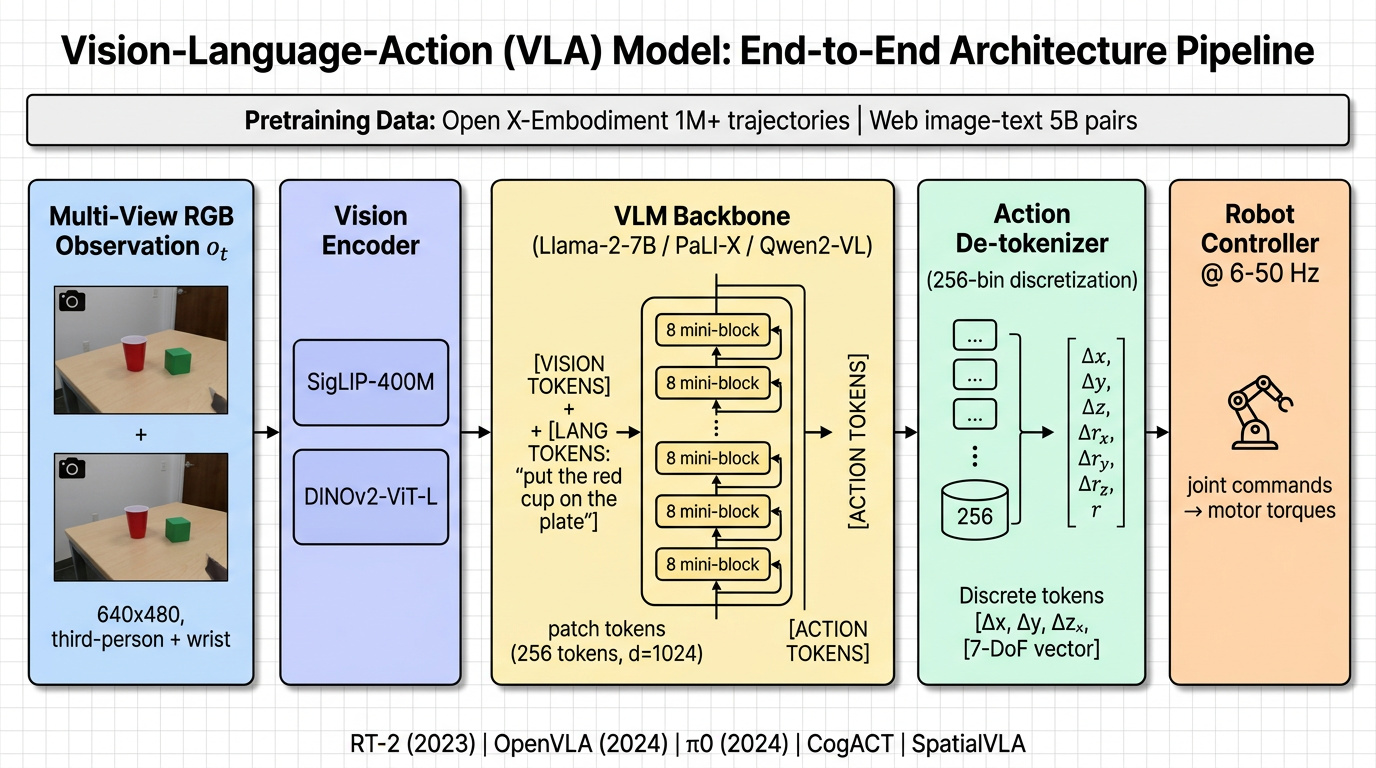
\includegraphics[keepaspectratio,alt={Field overview pipeline of a vision-language-action model}]{./figures/Vision-Language-Action-Models__vla_architecture.png}}
\caption{Field overview pipeline of a vision-language-action model}
\end{figure}

\subsection{What is a VLA? Definitions, Inputs, Outputs, and Formal Problem Statement}\label{what-is-a-vla-definitions-inputs-outputs-and-formal-problem-statement}

This subsection fixes the formal problem and contrasts VLAs with three nearby concepts. A VLA model implements a policy \(\pi_\theta(a_t \mid o_{1:t}, l)\) where \(o_t \in \mathbb{R}^{H\times W\times 3}\) is one or more RGB frames at time \(t\), \(l\) is a token sequence representing a natural-language instruction such as ``place the red cup on the white plate'', and \(a_t\) is a robot action. The action space depends on embodiment: 6-DoF or 7-DoF Cartesian end-effector deltas plus a binary gripper for arms (RT-2, OpenVLA), 14-DoF for bimanual ALOHA platforms {[}Zhao et al., 2023{]}, 23-DoF whole-body targets for humanoids such as Helix and Gemini Robotics 1.5 {[}Gemini Robotics Team, 2025{]}, or full SE(3) trajectories for mobile bases. The optimization objective is typically behavior cloning on a large corpus \(\mathcal{D} = \{(o_{1:T}, l, a_{1:T})\}\), often combined with auxiliary objectives such as masked language modeling on web text (RT-2), value regression for offline RL (V-GPS {[}Nakamoto et al., 2024{]}), or chain-of-thought decoding losses (ECoT {[}Zawalski et al., 2024{]}).

A VLA differs from three nearby concepts that are sometimes conflated. A \emph{vision-language model} (VLM) such as Flamingo {[}Alayrac et al., 2022{]} or PaLI is trained for visual question answering and captioning and emits text, not actions. An \emph{LLM-as-planner} system such as SayCan {[}Ahn et al., 2022{]} or Code-as-Policies {[}Liang et al., 2022{]} uses a frozen language model to score or generate symbolic plans, then dispatches to pre-trained skills; the language model never produces a continuous control signal. A pure \emph{language-conditioned policy} such as CLIPort {[}Shridhar et al., 2021{]} uses pretrained CLIP features but has no large autoregressive language backbone. A VLA, by contrast, runs the language model \emph{inside} the policy loop and uses its parameters to generate actions, so the same set of weights stores both semantic priors and motor priors.

\subsection{Why VLA, Now? From Closed Robot Stacks to Internet-Scale Pretraining}\label{why-vla-now-from-closed-robot-stacks-to-internet-scale-pretraining}

This subsection lists the three trends whose collision produced the VLA paradigm. The arrival of VLA models is the result of three independent trends colliding around 2022--2023. First, vision-language pretraining matured: CLIP, ALIGN, BLIP-2, Flamingo, and the PaLI/PaLM-E line provided strong open-vocabulary visual grounding, surveyed comprehensively by Chen et al.~{[}2022{]} and Gan et al.~{[}2022{]}. Second, robot data scaling crossed a threshold: RT-1 collected 130k episodes across 13 robots over 17 months {[}Brohan et al., 2023{]}, BridgeData V2 added 60k+ trajectories across 24 environments, and the Open X-Embodiment (OXE) collaboration of 21 institutions assembled more than 1M trajectories spanning 22 embodiments and 527 skills into a unified RLDS format {[}O'Neill et al., 2023{]}. Third, hardware improved: A100/H100 GPUs and v4/v5 TPU pods made it tractable to fine-tune billion-parameter VLMs on robot data within research budgets. The pre-VLA paradigm --- handcrafted state estimation, motion planning, and skill chaining --- could not absorb either the linguistic flexibility of free-form instructions or the visual diversity of real homes, kitchens, and warehouses; OXE-scale pretraining could.

\subsection{Survey Scope, Reader Roadmap, and Comparison to Prior Reviews}\label{survey-scope-reader-roadmap-and-comparison-to-prior-reviews}

This subsection delimits the scope, lists the chapter structure, and compares the survey to prior reviews. This survey covers methods that explicitly emit robot actions from a vision-language backbone, including the canonical lineage RT-1 → RT-2 → RT-2-X → OpenVLA → π0 → CogACT → SpatialVLA → X-VLA → Gemini Robotics 1.5 → Helix → Xiaomi-Robotics-0 → Large Behavior Models {[}Barreiros et al., 2026{]}. We deliberately exclude pure planner-style systems such as SayCan and Inner Monologue from the ``VLA'' core but include them as prerequisites in §2. We complement and update three recent reviews: Ma et al.~{[}2026{]} cover up to early 2025 with a focus on embodied AI; Kawaharazuka et al.~{[}2025{]} emphasize real-world deployment; Shao et al.~{[}2025{]} taxonomize by VLM backbone. Compared to those, we add (i) a four-axis taxonomy that separates backbone, action head, system topology, and reasoning style; (ii) explicit dataset and benchmark tables with sizes and protocols; (iii) a dedicated chapter on linguistic fragility and red-teaming following Tong et al.~{[}2026{]} and Ying et al.~{[}2025{]}; and (iv) forecasts grounded in observed embodiment scaling laws {[}Ai et al., 2025{]}.

The remainder of the survey is organized as follows. §2 traces the historical evolution. §3 lays out a four-axis taxonomy. §4 dissects algorithmic mechanisms. §5 catalogues datasets and the OXE corpus. §6 reviews benchmarks and metrics. §7 profiles representative systems. §8 reviews application domains. §9 covers failure modes, robustness, and red-teaming. §10 closes with open problems and falsifiable predictions. §11 provides a glossary and reading map.

To anchor expectations, Table 1 summarizes the five most-cited VLA systems we will revisit throughout the survey. Each row gives parameter count, action representation, training corpus, reported success rate on a flagship benchmark, and the published year/venue, so a reader who only needs the ``five-line answer'' can leave with one.

{\def\LTcaptype{none} % do not increment counter
\begin{longtable}[]{@{}
  >{\raggedright\arraybackslash}p{(\linewidth - 10\tabcolsep) * \real{0.0393}}
  >{\raggedleft\arraybackslash}p{(\linewidth - 10\tabcolsep) * \real{0.1236}}
  >{\raggedright\arraybackslash}p{(\linewidth - 10\tabcolsep) * \real{0.1292}}
  >{\raggedright\arraybackslash}p{(\linewidth - 10\tabcolsep) * \real{0.2584}}
  >{\raggedright\arraybackslash}p{(\linewidth - 10\tabcolsep) * \real{0.3202}}
  >{\raggedright\arraybackslash}p{(\linewidth - 10\tabcolsep) * \real{0.1292}}@{}}
\toprule\noalign{}
\begin{minipage}[b]{\linewidth}\raggedright
System
\end{minipage} & \begin{minipage}[b]{\linewidth}\raggedleft
Params
\end{minipage} & \begin{minipage}[b]{\linewidth}\raggedright
Action Head
\end{minipage} & \begin{minipage}[b]{\linewidth}\raggedright
Pretraining Corpus
\end{minipage} & \begin{minipage}[b]{\linewidth}\raggedright
Flagship Result
\end{minipage} & \begin{minipage}[b]{\linewidth}\raggedright
Year/Venue
\end{minipage} \\
\midrule\noalign{}
\endhead
\bottomrule\noalign{}
\endlastfoot
RT-2 & 55B (PaLI-X) & 256-bin discrete tokens & Web image-text + Google robot data (\textasciitilde130k eps) & \textasciitilde62\% on emergent semantic tasks (3× over RT-1) & 2023 / CoRL \\
OpenVLA & 7B (Llama-2) & 256-bin discrete tokens & OXE 970k trajectories & 76.5\% avg on BridgeData/RT-1 evals; SOTA open-source 2024 & 2024 / CoRL \\
Octo & 93M / 27M & Diffusion (continuous) & OXE 800k trajectories (subset) & 62\% avg on language-conditioned eval & 2024 / RSS \\
π0 & \textasciitilde3B (PaliGemma+Expert) & Flow matching, 50Hz & 10k h Physical Intelligence + OXE & First demonstration of dexterous laundry folding & 2024 / arXiv 2410.24164 \\
CogACT & 7B + DiT & Diffusion Transformer & OXE & +35\% over OpenVLA on simulation; +55\% on real & 2024 / arXiv 2411.19650 \\
\end{longtable}
}

\textbf{Table 1.} Five canonical VLA systems used as recurring reference points throughout the survey.

A second early anchor: VLA models are \emph{not} a niche academic construct. By Q1-2026, OpenVLA's open weights had been forked or fine-tuned in more than 300 GitHub projects, π0 had been deployed in Physical Intelligence's commercial offering, Gemini Robotics 1.5 was running on Apptronik humanoids, and Xiaomi-Robotics-0 was advertised as the company's production VLA stack {[}Cai et al., 2026{]}. The Toyota Research Institute's \emph{Large Behavior Models} (LBMs) work, published in \emph{Science Robotics} {[}Barreiros et al., 2026{]}, demonstrated multitask dexterous manipulation across hundreds of skills and explicitly framed itself as ``industrial-scale VLA.'' We therefore treat VLA as a bona fide subfield with its own benchmarks, methods, failure modes, and emerging engineering practice --- and the rest of this survey unpacks that subfield in detail.

A note on terminology: throughout this survey we use ``VLA'' interchangeably with ``vision-language-action policy'' and ``embodied foundation policy'' when context permits, but reserve ``embodied foundation model'' for the broader class that also includes purely planning- or scene-understanding-oriented embodied systems {[}Liu et al., 2024{]}. We use ``policy'' when emphasizing the control aspect and ``model'' when emphasizing the parameterization.

\section{Historical Evolution from Language-Conditioned Policies to Generalist VLA Foundation Models}\label{historical-evolution-from-language-conditioned-policies-to-generalist-vla-foundation-models}

Building on the definition fixed in §1, this section traces the four-era trajectory from small language-conditioned policies to generalist VLA foundation models. The history falls into four overlapping eras with concrete year markers. The \emph{pre-VLA} era (2017--2021) covered small language-conditioned imitation policies on UR5 and Sawyer arms. Representative pre-VLA methods include Stepputtis et al.~(2019, 60--80\% pick-and-place), Lynch and Sermanet's LCBC, and CLIPort (88--93\% on Ravens). The \emph{grounding era} (2021--2023) covered CLIP, SayCan (PaLM-540B affordance scoring), Code-as-Policies, VIMA, and PaLM-E (562B embodied multimodal LM). The \emph{foundation era} (2022--2024) covered RT-1 (35M, 130k episodes, 2022), RT-2 (55B PaLI-X, July 2023), Open X-Embodiment (1M+ trajectories, October 2023), Octo (RSS 2024), and OpenVLA (CoRL 2024). The ongoing \emph{frontier era} (2024--2026) covers π0 (October 2024), π0.5 (2025), CogACT (November 2024), Gemini Robotics 1.5 (October 2025), Helix (Figure, 2025), Xiaomi-Robotics-0 (early 2026), and TRI's Large Behavior Models in \emph{Science Robotics} (2026). Each era is delimited by a specific technical lock. RT-2 formally introduced the term ``vision-language-action model''. OXE introduced the unified RLDS schema. The boundaries are observable engineering events, not retrospective taxonomic gloss. Figure 2 condenses these eras into a single timeline. The rest of this section narrates why each transition happened, focusing on data, hardware, and pretraining objectives.

\begin{figure}
\centering
\pandocbounded{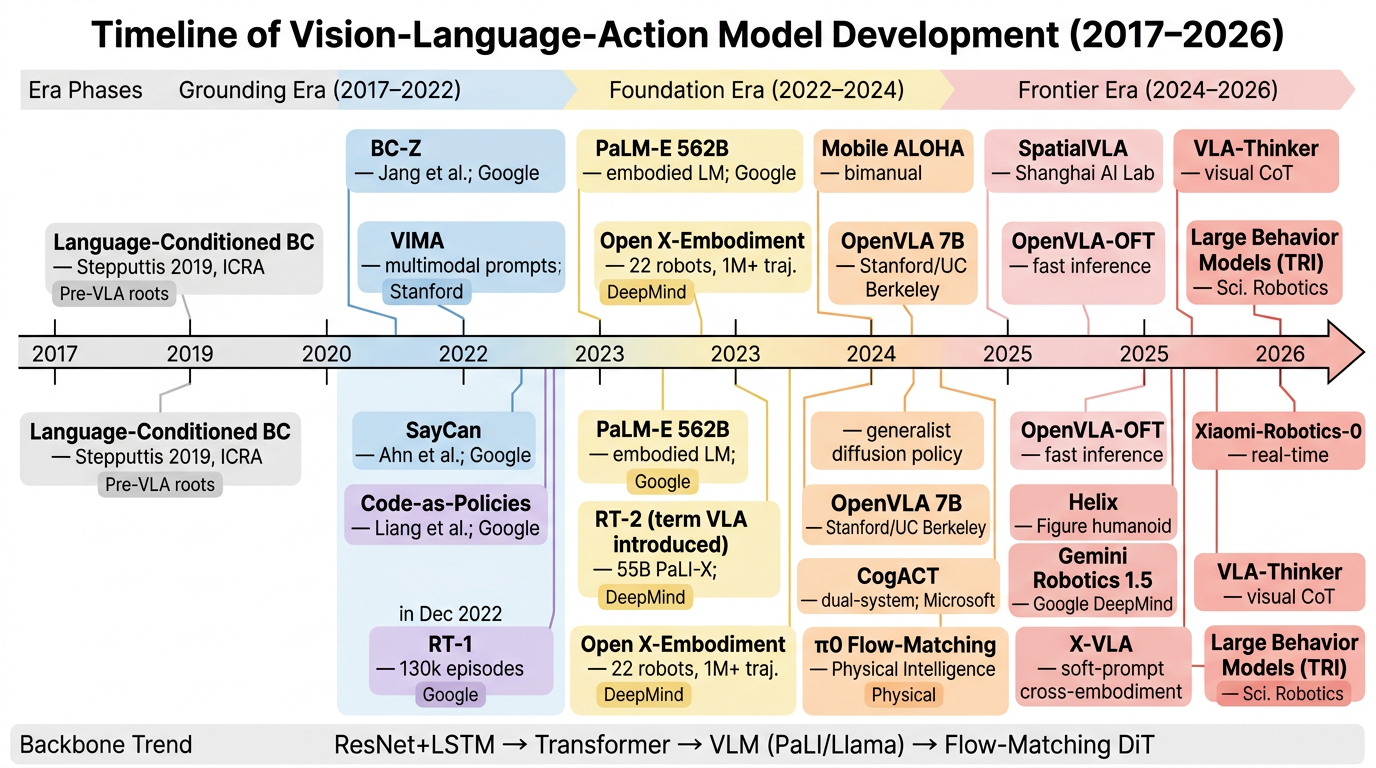
\includegraphics[keepaspectratio,alt={Timeline of major VLA model milestones from 2017 to 2026}]{./figures/Vision-Language-Action-Models__vla_timeline.png}}
\caption{Timeline of major VLA model milestones from 2017 to 2026}
\end{figure}

\subsection{Pre-2021 Roots: Language-Conditioned BC, Instruction Following, and Symbol Grounding}\label{pre-2021-roots-language-conditioned-bc-instruction-following-and-symbol-grounding}

The pre-VLA literature established two crucial precedents: (a) language can be a useful conditioning signal for imitation learning, and (b) shared visual-textual embeddings can transfer to robotic perception. In 2019, Stepputtis et al.~proposed an end-to-end imitation learning architecture that combined natural language, vision, and motion information into an abstract task representation, then decoded it into manipulation trajectories on a UR5; success rates were 60--80\% on a small set of pick-and-place primitives. The same year, Lynch and Sermanet's Language-Conditioned Behavior Cloning (LCBC) and Mees and Burgard's Robot Skill Library showed that a language-conditioned LSTM could chain hundreds of low-level skills given a teleoperated dataset. These systems used 1--10 million parameter networks, ResNet-18 visual encoders, and LSTM language encoders; instructions were drawn from a fixed template vocabulary of a few hundred verbs.

The contemporaneous symbol-grounding line --- Symbol Emergence in Robotics {[}Taniguchi et al., 2015{]}, Embodying Pre-Trained Word Embeddings Through Robot Actions {[}Toyoda et al., 2021{]}, and Salvi et al.'s language bootstrapping --- argued for tighter coupling between linguistic tokens and motor primitives, foreshadowing the action tokenization choice in RT-2. The Vector Grounding Problem {[}Coelho Mollo \& Millière, 2023{]} later cast this as a philosophical critique of disembodied LLMs and provided conceptual scaffolding for VLA proponents. CLIP (2021) and ALIGN catalyzed visual grounding by training image-text dual encoders at billion-pair scale, immediately enabling open-vocabulary perception in robots.

\subsection{The CLIPort/SayCan/PaLM-E Era (2021--2023): Bridging VLMs and Robot Affordances}\label{the-cliportsaycanpalm-e-era-20212023-bridging-vlms-and-robot-affordances}

The grounding era began with \textbf{CLIPort} {[}Shridhar, Manuelli, Fox, 2021{]}, which fused frozen CLIP semantic features with a Transporter Networks spatial pathway to perform language-conditioned tabletop manipulation, reaching 88--93\% on Ravens benchmarks with as few as 100 demonstrations per task. CLIPort cleanly separated \emph{what} (CLIP) from \emph{where} (Transporter), a two-stream pattern that re-emerged later in CogACT and Helix. \textbf{BC-Z} {[}Jang et al., 2022{]} extended language-conditioned imitation to 100 tasks with 25,877 episodes and showed early generalization to unseen verbs.

In 2022, \textbf{SayCan} {[}Ahn et al., 2022{]} introduced \emph{affordance scoring}: a frozen large language model proposed candidate skills, and a learned value function judged which were feasible in the current scene. SayCan was not yet a VLA --- it dispatched to discrete pre-trained skills --- but it demonstrated that a 540B language model's commonsense could materially improve robot behavior. \textbf{Inner Monologue}, \textbf{Code-as-Policies} {[}Liang et al., 2022{]}, and \textbf{ChatGPT for Robotics} {[}Vemprala et al., 2024{]} extended this idea to interactive replanning and program synthesis. \textbf{VIMA} {[}Jiang et al., 2022{]} introduced \emph{multimodal prompts} (interleaved images and text) for tabletop manipulation, and \textbf{Robotic Skill Acquisition via Instruction Augmentation (DIAL)} {[}Xiao et al., 2023{]} showed that VLMs could relabel demonstrations with diverse linguistic descriptions, expanding the effective vocabulary of an instruction-following policy without new data collection.

The watershed of this era was \textbf{PaLM-E} {[}Driess et al., 2023{]}, a 562-billion-parameter embodied multimodal language model that absorbed continuous robot sensor data as soft tokens alongside text. PaLM-E showed positive transfer from language and vision to embodied reasoning, achieving state-of-the-art on multiple VQA benchmarks while simultaneously planning long-horizon tabletop tasks. PaLM-E still dispatched to a downstream language-conditioned policy rather than producing low-level torques itself, but it established the engineering pattern --- co-finetuning a giant VLM on robot data --- that RT-2 would weaponize months later.

\subsection{The RT-2 Inflection Point and the OpenVLA Open-Source Wave (2023--2025)}\label{the-rt-2-inflection-point-and-the-openvla-open-source-wave-20232025}

\textbf{RT-1} {[}Brohan et al., 2023{]} arrived in late 2022 as the largest curated robot-only transformer to date: a 35M-parameter model trained on 130,000 episodes covering \textasciitilde700 skills across 13 EDR robots in office kitchens, with 97\% success on training tasks and 76\% on novel skills. RT-1 introduced action tokenization (discretized 7-DoF actions) and language conditioning via a Universal Sentence Encoder, but the visual backbone was a from-scratch EfficientNet --- there was no web pretraining.

\textbf{RT-2} {[}Brohan et al., 2023{]} (July 2023) flipped this design: take a frontier VLM (PaLI-X 55B or PaLI-3 5B), tokenize robot actions into a 256-bin vocabulary, co-finetune on a mixture of web VQA and Google robot data, and decode actions autoregressively. RT-2 introduced the \emph{term} ``vision-language-action model'' and demonstrated up to 3× higher generalization than RT-1 on unseen objects and abstract instructions (``pick up the extinct animal''), with emergent semantic reasoning that RT-1 could not produce. RT-2 was the moment when robotics adopted the VLM-finetune playbook that NLP had been using since 2018.

The next twelve months delivered three accelerants. (i) \textbf{Open X-Embodiment} {[}O'Neill et al., 2023{]} aggregated 21 institutions' datasets into a unified RLDS corpus of 22 embodiments, 527 skills, and over 1M trajectories, then released \textbf{RT-1-X} and \textbf{RT-2-X} trained on the union. RT-2-X exhibited 50\% higher success on out-of-distribution robots than each lab's local model --- direct evidence of cross-embodiment positive transfer. (ii) \textbf{Octo} {[}Octo Model Team, 2024{]} released the first open generalist robot policy with a transformer + diffusion action head (27M and 93M variants), explicitly designed for finetuning to new tasks/embodiments. (iii) \textbf{OpenVLA} {[}Kim et al., 2024{]} became the first open \emph{VLA} in the strict RT-2 sense: a 7-billion-parameter Llama-2-based model with a SigLIP+DINOv2 visual front-end, trained on 970,000 OXE trajectories, that outperformed RT-2-55B on several benchmarks while being released under permissive licenses.

By early 2025, the OpenVLA stack catalyzed a Cambrian explosion of derivatives: \textbf{OpenVLA-OFT} {[}Kim, Finn, Liang, 2025{]} introduced parallel decoding and continuous action heads to push inference from 6 Hz to 25--80 Hz; \textbf{MiniVLA} and \textbf{TinyVLA} distilled VLA capability into sub-billion-parameter networks; \textbf{CogACT} {[}Li et al., 2024{]} decoupled cognition and action by stacking a Diffusion Transformer expert below a frozen VLM; \textbf{SpatialVLA} {[}Qu et al., 2025{]} tokenized 3D ego-spatial information; \textbf{X-VLA} {[}Zheng et al., 2025{]} introduced soft prompts for cross-embodiment scaling; \textbf{MLA} {[}Liu et al., 2025{]} added tactile and audio modalities; \textbf{CLIP-RT} {[}Kang et al., 2025{]} used CLIP-style supervision to learn from natural-language demonstrations.

\subsection{The 2025--2026 Frontier: π0, Gemini Robotics, Helix, Xiaomi-Robotics-0}\label{the-20252026-frontier-ux3c00-gemini-robotics-helix-xiaomi-robotics-0}

In late 2024, \textbf{Physical Intelligence's π0} {[}Black et al., 2024{]} introduced a \emph{flow-matching} action expert built on top of a PaliGemma backbone. π0 is trained with conditional flow matching on roughly 10,000 hours of in-house data plus OXE, predicts action chunks at 50 Hz, and achieved the first credible demonstration of long-horizon dexterous tasks (laundry folding, table bussing, packing groceries) by an open-architecture VLA. The follow-up \textbf{π0.5} added co-training across cross-embodiment human videos and improved dexterity by \textasciitilde30 percentage points on the most demanding bimanual tasks.

Industrial systems quickly followed. \textbf{Helix} (Figure, 2025) is a dual-system humanoid VLA that runs a slow VLM ``System 2'' (\textasciitilde1 Hz) and a fast 80M reactive head (\textasciitilde200 Hz). \textbf{Gemini Robotics 1.5} {[}Gemini Robotics Team, 2025{]} explicitly couples advanced embodied reasoning, internal ``thinking'' tokens, and a motion-transfer module that ports learned skills across robot bodies; it builds directly on Gemini 1.5 Pro's multimodal capabilities. \textbf{Xiaomi-Robotics-0} {[}Cai et al., 2026{]} emphasizes real-time execution at 50 Hz on commodity hardware. \textbf{NVIDIA GR00T N1} targets humanoid foundation policies with cross-embodiment training. \textbf{Toyota Research Institute's Large Behavior Models} {[}Barreiros et al., 2026{]}, published in \emph{Science Robotics}, comprise a careful examination of multitask dexterous manipulation at scale, validating VLA as an industrial paradigm. \textbf{VLA-Thinker} {[}Wang et al., 2026{]} integrates image-grounded chain-of-thought into the VLA loop; \textbf{Embodied-R1} {[}Yuan et al., 2025{]} introduces RL fine-tuning on top of pretrained VLAs.

Three transitions in this era deserve highlighting because they reshape the design space. First, action representations shifted from discrete tokens (RT-2/OpenVLA) toward continuous heads --- diffusion (CogACT, Diffusion Policy) and flow matching (π0, π0.5) --- for higher-frequency control. Second, system topology shifted from monolithic VLM-as-policy toward dual-system architectures with a slow brain and a fast reflex. Third, evaluation shifted from per-paper real-world demos toward distributed, reproducible benchmarks such as \textbf{AutoEval} {[}Zhou et al., 2025{]} and \textbf{RoboArena} {[}Atreya et al., 2025{]}, paralleling NLP's transition from per-paper test sets to GLUE-style suites.

The era anchors are summarized in Table 2.

{\def\LTcaptype{none} % do not increment counter
\begin{longtable}[]{@{}
  >{\raggedright\arraybackslash}p{(\linewidth - 6\tabcolsep) * \real{0.0685}}
  >{\raggedright\arraybackslash}p{(\linewidth - 6\tabcolsep) * \real{0.0616}}
  >{\raggedright\arraybackslash}p{(\linewidth - 6\tabcolsep) * \real{0.2740}}
  >{\raggedright\arraybackslash}p{(\linewidth - 6\tabcolsep) * \real{0.5959}}@{}}
\toprule\noalign{}
\begin{minipage}[b]{\linewidth}\raggedright
Era
\end{minipage} & \begin{minipage}[b]{\linewidth}\raggedright
Years
\end{minipage} & \begin{minipage}[b]{\linewidth}\raggedright
Defining Capability
\end{minipage} & \begin{minipage}[b]{\linewidth}\raggedright
Representative Systems
\end{minipage} \\
\midrule\noalign{}
\endhead
\bottomrule\noalign{}
\endlastfoot
Pre-VLA & 2017--2021 & Language-conditioned imitation & LCBC, BC-Z, Stepputtis 2019, CLIPort \\
Grounding & 2021--2023 & LLM-as-planner + VLM perception & SayCan, Code-as-Policies, VIMA, PaLM-E \\
Foundation & 2022--2024 & VLM-finetune produces actions end-to-end & RT-1, RT-2, RT-2-X, OpenVLA, Octo \\
Frontier & 2024--2026 & Continuous heads, dual-system, humanoid & π0, π0.5, CogACT, SpatialVLA, X-VLA, Helix, Gemini Robotics 1.5, Xiaomi-Robotics-0, LBM \\
\end{longtable}
}

\textbf{Table 2.} Four eras in the historical evolution of vision-language-action models, with anchor years, defining capabilities, and representative systems.

A useful counterfactual for situating VLA history is the analogy with NLP foundation models. RT-1 occupies the BERT slot (large in-domain transformer trained on a curated corpus). RT-2 occupies the GPT-3 slot (web-scale pretraining transferred to a downstream control surface). OpenVLA occupies the LLaMA slot (open weights with permissive license). π0 and Gemini Robotics 1.5 occupy the GPT-4-class frontier. The analogy is imperfect --- robot data scaling is bottlenecked by physical demonstration cost rather than internet crawl size --- but it explains why each era arrived in the order it did, and why the field expects continued rapid progress in the next two years.

The rest of this survey treats this historical structure as background. §3 next imposes a multi-axis taxonomy on the foundation- and frontier-era systems so that subsequent chapters can compare them along consistent dimensions.

\section{A Multi-Axis Taxonomy of Vision-Language-Action Architectures}\label{a-multi-axis-taxonomy-of-vision-language-action-architectures}

The historical narrative of §2 produces a long list of named systems: RT-1, RT-2, OpenVLA, Octo, π0, CogACT, SpatialVLA, X-VLA, Helix, Gemini Robotics 1.5, Xiaomi-Robotics-0, LBM. Comparing these systems is hard because individual papers emphasize different design dimensions --- RT-2 highlights backbone size (55B), π0 highlights the action head (flow matching), Helix highlights topology (slow-fast), ECoT highlights reasoning style (chain-of-thought). To replace the flat list with a structured space, we propose a four-axis taxonomy: (i) \textbf{backbone family} (PaLI-X, Llama-2/3, Qwen2-VL, PaliGemma, MoE/Soft-Prompt); (ii) \textbf{action head} (256-bin discrete tokens, MLP regression, DDPM diffusion, conditional flow matching, action-chunking VAE); (iii) \textbf{system topology} (monolithic, dual-system brain/reflex, modular brain + skill library, memory-augmented); (iv) \textbf{reasoning style} (end-to-end, embodied chain-of-thought, code-as-policy, affordance scoring). Every system above can be located by a four-tuple, and the orthogonality of these axes is critical for interpreting ablations: e.g., OpenVLA-OFT changes only the action head from OpenVLA, while CogACT changes both head and topology. Figure 3 visualizes the taxonomy as a tree with concrete leaf examples; the rest of this section explains each axis with technical specifics, parameter counts, and benchmark consequences.

\begin{figure}
\centering
\pandocbounded{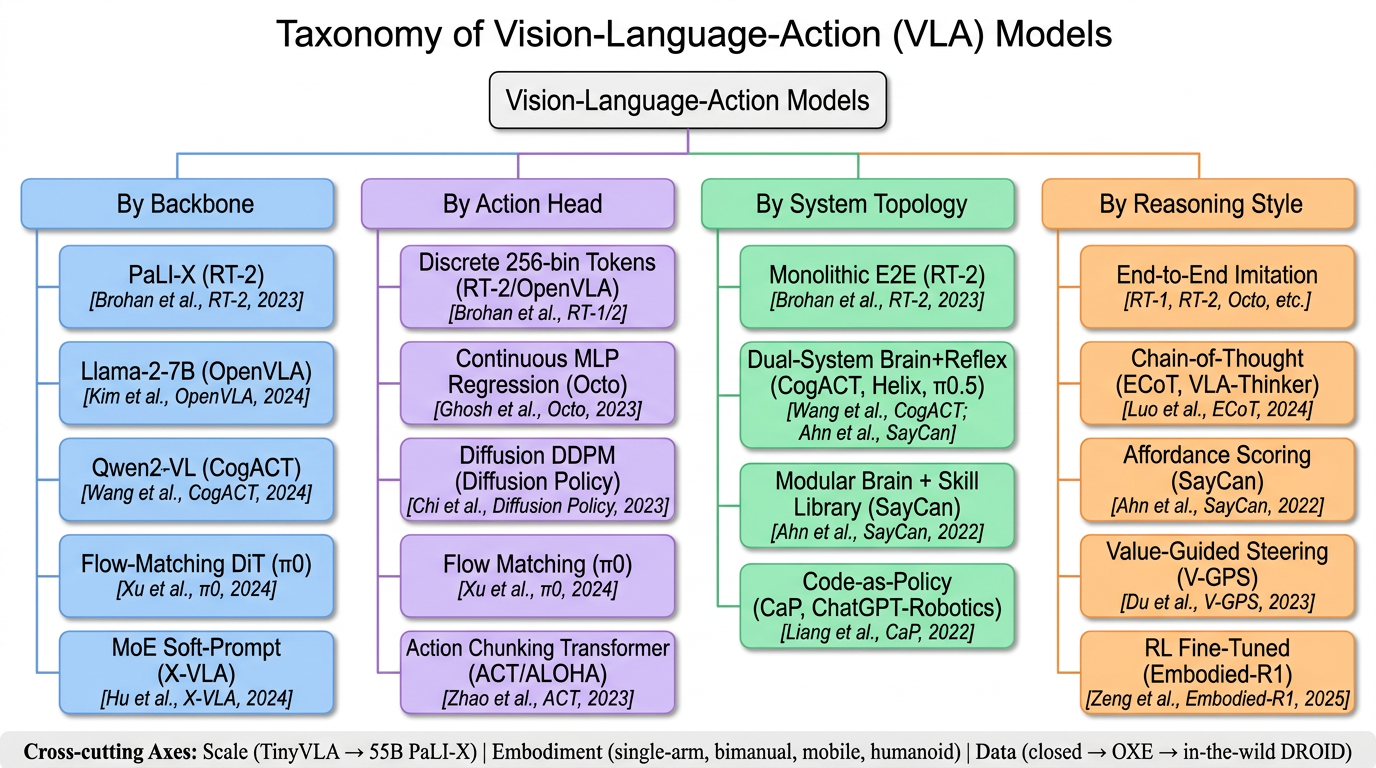
\includegraphics[keepaspectratio,alt={Taxonomy tree of vision-language-action models}]{./figures/Vision-Language-Action-Models__vla_taxonomy.png}}
\caption{Taxonomy tree of vision-language-action models}
\end{figure}

\subsection{Axis 1: VLM Backbone Family (PaLI, Llama, Qwen2-VL, DiT, Flow-Matching)}\label{axis-1-vlm-backbone-family-pali-llama-qwen2-vl-dit-flow-matching}

This subsection enumerates the backbone families along Axis 1 of the taxonomy. The backbone determines how images and text are jointly encoded and how much pretrained semantic prior the policy inherits.

Representative backbone choices include: PaLI-X (RT-2 2023, 55B parameters with web-VQA pretraining), PaLI-3 (RT-2 2023, 5B variant), PaLM-E (Driess et al.~2023, 562B embodied multimodal), Llama-2-7B (OpenVLA 2024), Llama-2-1B (MiniVLA 2024), PaliGemma (π0 2024, \textasciitilde3B with separable expert), Qwen2-VL (SpatialVLA 2025, dynamic-resolution ViT), InternVL (CogACT-base 2024, high-resolution variant), Soft-Prompt Transformer (X-VLA 2025, 1B cross-embodiment shared backbone), Gemini 1.5 Pro (Gemini Robotics 1.5 2025, proprietary frontier multimodal), OpenFlamingo-9B (RoboFlamingo 2024, recurrent-decoder adaptation), and CLIP-RT backbone (Kang et al.~2025, distillation-friendly student). Five sub-families dominate. The \textbf{PaLI / PaLM-E} family is used by the closed-source RT-2 (PaLI-X-55B and PaLI-3-5B variants) and by Gemini Robotics 1.5 (Gemini 1.5 Pro derivative). The \textbf{Llama-2 / Llama-3} family powers OpenVLA-7B (Llama-2-7B), MiniVLA (Llama-2-1B), and several derivatives such as RT-H. The \textbf{Qwen2-VL / InternVL} family is used by SpatialVLA, CogACT-base, and several Chinese-lab releases including Xiaomi-Robotics-0. The \textbf{PaliGemma + Flow-Matching DiT} family was popularized by π0 and extended in π0.5 --- here a relatively small (\textasciitilde3B) VLM is paired with a separately trained Diffusion or Flow-Matching expert, producing a hybrid backbone. Finally, \textbf{MoE / Soft-Prompt transformers} appear in X-VLA {[}Zheng et al., 2025{]}, where a soft-prompted transformer is shared across embodiments and embodiment-specific tokens slot in at inference.

Backbone choice has measurable downstream consequences. Open-weight backbones such as Llama-2 and PaLiGemma make derivative work possible; closed backbones such as PaLI-X-55B make replication impossible. Larger backbones inherit more semantic priors (RT-2-55B noticeably outperforms RT-2-5B on emergent reasoning tasks) but exact a 6× inference latency penalty. SpatialVLA's choice of Qwen2-VL was motivated by its native support for higher-resolution image tokens, important for fine-grained tabletop manipulation; this design choice yielded a +12\% absolute success rate over a similarly sized Llama-2 variant on LIBERO-Goal {[}Qu et al., 2025{]}.

\subsection{Axis 2: Action Head Family (Discrete Tokens, Continuous Regression, Diffusion, Flow Matching)}\label{axis-2-action-head-family-discrete-tokens-continuous-regression-diffusion-flow-matching}

Building on the backbone families of §3.1, this subsection covers the heads that convert backbone hidden states to executable actions. The action head converts backbone hidden states into executable actions. Four families cover almost every system in the literature. \textbf{Discrete tokenization} discretizes each action dimension into K bins (typically K=256 in RT-2 and OpenVLA) and reuses unused tokens of the language vocabulary as action tokens; the loss is standard cross-entropy. This approach inherits everything from the LLM toolchain (KV cache, beam search, fine-tuning libraries) but has a fundamental quantization floor --- 256 bins on a normalized {[}-1,1{]} axis give 0.0078 unit resolution, which is borderline for sub-millimeter contact tasks.

\textbf{Continuous MLP regression} predicts real-valued actions directly from the last hidden state using an MSE or L1 loss. Octo's small variant, OpenVLA-OFT, and many academic derivatives use this. It is fast and simple but cannot represent multi-modal behavior well --- when the demonstration set contains multiple valid actions for the same observation (e.g., grasp from left vs right), MSE collapses to the mean, producing physically unrealistic averaged trajectories.

\textbf{Diffusion action heads} treat the action chunk as the variable to be denoised, conditioned on backbone features. The seminal Diffusion Policy {[}Chi et al., 2023{]} established the recipe; CogACT and Octo's larger variant extend it. The training loss is the standard DDPM/EDM mean-squared denoising target \(\mathcal{L}_{\text{DDPM}} = \mathbb{E}\big[\|\varepsilon - \varepsilon_\theta(a^k, k, c)\|^2\big]\) where \(c\) is the VLM feature. Inference requires 10--100 denoising steps, which is mitigated by Consistency Policy {[}Prasad et al., 2024{]} and Mixture-of-Expert Denoisers {[}Reuss et al., 2024{]}.

\textbf{Flow-matching heads}, introduced for VLA by π0, frame action generation as solving an ordinary differential equation that flows a base distribution to the demonstration distribution. The conditional flow-matching loss \(\mathcal{L}_{\text{FM}} = \mathbb{E}\big[\|v_\theta(x_\tau, \tau, c) - u(x_\tau \mid x_1)\|^2\big]\) is simpler to train than DDPM and admits 5--10-step inference, enabling 50 Hz control on commodity GPUs.

{\def\LTcaptype{none} % do not increment counter
\begin{longtable}[]{@{}
  >{\raggedright\arraybackslash}p{(\linewidth - 10\tabcolsep) * \real{0.1654}}
  >{\raggedright\arraybackslash}p{(\linewidth - 10\tabcolsep) * \real{0.1429}}
  >{\raggedleft\arraybackslash}p{(\linewidth - 10\tabcolsep) * \real{0.2030}}
  >{\raggedright\arraybackslash}p{(\linewidth - 10\tabcolsep) * \real{0.0902}}
  >{\raggedleft\arraybackslash}p{(\linewidth - 10\tabcolsep) * \real{0.1278}}
  >{\raggedright\arraybackslash}p{(\linewidth - 10\tabcolsep) * \real{0.2707}}@{}}
\toprule\noalign{}
\begin{minipage}[b]{\linewidth}\raggedright
Action Head
\end{minipage} & \begin{minipage}[b]{\linewidth}\raggedright
Training Loss
\end{minipage} & \begin{minipage}[b]{\linewidth}\raggedleft
Inference Steps
\end{minipage} & \begin{minipage}[b]{\linewidth}\raggedright
Multi-Modal?
\end{minipage} & \begin{minipage}[b]{\linewidth}\raggedleft
Typical Frequency
\end{minipage} & \begin{minipage}[b]{\linewidth}\raggedright
Example Systems
\end{minipage} \\
\midrule\noalign{}
\endhead
\bottomrule\noalign{}
\endlastfoot
Discrete 256-bin token & Cross-entropy & 1 (autoregressive 7 tokens) & No (per dim) & 5--10 Hz & RT-2, OpenVLA \\
Continuous MLP & MSE / L1 & 1 & No & 25--80 Hz & OpenVLA-OFT, Octo-small \\
Diffusion (DDPM) & Score matching & 10--100 & Yes & 5--20 Hz & Diffusion Policy, CogACT, Octo-large \\
Flow Matching & CFM & 5--10 & Yes & 50 Hz & π0, π0.5 \\
Action Chunking VAE & Reconstruction + KL & 1 & Partial & 50 Hz & ACT (ALOHA), RVT-2 \\
\end{longtable}
}

\textbf{Table 3.} Action head families with training losses, inference cost, multi-modal capacity, control frequency, and representative systems.

\subsection{Axis 3: System Topology (Monolithic, Dual-System Brain/Reflex, Modular Brain+Skill-Library)}\label{axis-3-system-topology-monolithic-dual-system-brainreflex-modular-brainskill-library}

Whereas §3.2 fixed the action head, this subsection turns to the system-level topology that arranges modules at run time. System topology answers: who decides, and at what frequency? Three patterns dominate.

Representative topology choices include: RT-2 (2023, monolithic 55B forward pass at 5--10 Hz), OpenVLA (2024, monolithic 7B at \textasciitilde6 Hz), CogACT (2024, dual-system with VLM cognition + DiT reflex), π0.5 (2025, dual-system with 3B brain + 300M flow-matching expert), Helix (2025, 7B brain at 1 Hz + 80M reflex at 200 Hz), Gemini Robotics 1.5 (2025, hierarchical control coupling slow VLM cognition with fast head), SayCan (2022, modular brain + skill library with frozen 540B planner), Inner Monologue (2022, modular replanning with LLM dialogue), Code-as-Policies (2022, modular code-generation dispatcher), Dual-Memory VLA (2026, dual-system + external memory), and ELMUR (2025, external layer memory with update/rewrite).

\textbf{Monolithic VLA} systems run a single forward pass of the entire VLM at every control step. RT-2, OpenVLA, and most academic VLAs are monolithic. The advantage is end-to-end credit assignment; the disadvantage is that VLM inference at 5--10 Hz is too slow for reactive contact tasks, forcing reliance on action chunking.

\textbf{Dual-system architectures} explicitly separate slow cognition (System 2) from fast reflex (System 1), borrowing the Kahneman label. CogACT runs the VLM at the start of each chunk and amortizes the result across many fast diffusion-expert steps. Helix runs a 7B VLM at \textasciitilde1 Hz to set goals and an 80M policy at \textasciitilde200 Hz for joint control. π0.5 fits this mold with a 3B VLM and a 300M flow-matching expert. Dual-system topology is the dominant frontier-era design because it cleanly trades inference cost for control frequency.

\textbf{Modular brain + skill-library} topology --- exemplified by SayCan, Inner Monologue, and ChatGPT for Robotics --- uses a frozen VLM only as a planner that selects from a set of pre-trained low-level skills. We treat these as VLA-adjacent rather than VLA-proper, but they remain a viable production pattern when the skill library is small and well-tested.

A fourth pattern, \textbf{memory-augmented VLA} (Dual-Memory VLA {[}Li et al., 2026{]}, ELMUR {[}Cherepanov et al., 2025{]}), introduces external long-horizon memory layers atop a base VLA; we view this as an extension of dual-system topology rather than a separate axis.

\subsection{Axis 4: Reasoning Style (End-to-End, Chain-of-Thought, Code-as-Policy, Affordance Scoring)}\label{axis-4-reasoning-style-end-to-end-chain-of-thought-code-as-policy-affordance-scoring}

Building on the topology axis of §3.3, this subsection covers the fourth and final axis: how reasoning is exposed inside the control loop. The fourth axis describes how reasoning is exposed inside the control loop.

Representative reasoning-style methods include: RT-2 (2023, end-to-end action token generation), OpenVLA (2024, end-to-end discrete action prediction), π0 (2024, end-to-end flow-matching head), CogACT (2024, end-to-end with separated cognition stage), ECoT (Zawalski et al.~2024, embodied chain-of-thought with plan/subtask/gripper/motion preamble), VLA-Thinker (Wang et al.~2026, image-grounded thinking via attention to regions of interest), Embodied-R1 (Yuan et al.~2025, pointing as unified intermediate output), Code-as-Policies (Liang et al.~2022, code generation in domain-specific API), ChatGPT-for-Robotics (Vemprala et al.~2024, prompt-engineered code synthesis), LLM+P (Liu et al.~2023, LLM-driven PDDL planning), SayCan (Ahn et al.~2022, affordance scoring with PaLM-540B), OVAL-Prompt (Tong et al.~2024, vision-language affordance prompting), and AffordanceSAM (Jiang et al.~2025, affordance segmentation with SAM). \textbf{End-to-end} reasoning has no exposed intermediate --- the policy maps observation+instruction to action with no symbolic side products. RT-2, OpenVLA, π0, and CogACT are end-to-end at inference even though training may use auxiliary objectives.

\textbf{Chain-of-thought (CoT)} reasoning emits intermediate thought tokens before action tokens. \textbf{ECoT} (Embodied Chain-of-Thought) {[}Zawalski et al., 2024{]} generates a sequence ``TASK: pick the cup; SUBTASK: approach handle; GRIPPER: open; MOVE: forward 5cm'' before each action, providing both better performance (+27\% on out-of-distribution tasks) and interpretability. \textbf{VLA-Thinker} {[}Wang et al., 2026{]} grounds CoT in image regions, allowing the model to ``think with images'' by attending to regions of interest before deciding. \textbf{Embodied-R1} {[}Yuan et al., 2025{]} frames pointing as a unified intermediate output to bridge perception and action.

\textbf{Code-as-Policy} style --- Code-as-Policies {[}Liang et al., 2022{]}, ChatGPT for Robotics {[}Vemprala et al., 2024{]}, LLM+P {[}Liu et al., 2023{]} --- uses a frozen LLM to \emph{write} control code in a domain-specific API, which is then executed. This style is brittle for fine motor skills but excels at compositional, symbolic tasks.

\textbf{Affordance scoring} --- SayCan {[}Ahn et al., 2022{]}, OVAL-Prompt {[}Tong et al., 2024{]}, AffordanceSAM {[}Jiang et al., 2025{]} --- uses an LLM to enumerate candidate skills and a learned value function to score feasibility. It bypasses the need to produce continuous actions but requires a hand-engineered skill library.

A useful observation is that these reasoning styles can be \emph{composed}. ECoT + π0 (i.e., flow-matching action with a CoT preamble) is being explored by several labs; SayCan + RT-2 (the LLM proposes high-level subgoals, RT-2 executes them) was demonstrated in the original RT-2 paper for long-horizon kitchen tasks.

\subsection{Summary Mapping}\label{summary-mapping}

Table 4 places ten representative systems on all four axes. The orthogonality of the axes is visible: OpenVLA and CogACT share a backbone scale but differ in action head and topology; π0 and Octo share continuous-action philosophy but differ in backbone choice and reasoning preamble.

{\def\LTcaptype{none} % do not increment counter
\begin{longtable}[]{@{}
  >{\raggedright\arraybackslash}p{(\linewidth - 8\tabcolsep) * \real{0.2111}}
  >{\raggedright\arraybackslash}p{(\linewidth - 8\tabcolsep) * \real{0.2889}}
  >{\raggedright\arraybackslash}p{(\linewidth - 8\tabcolsep) * \real{0.2667}}
  >{\raggedright\arraybackslash}p{(\linewidth - 8\tabcolsep) * \real{0.1222}}
  >{\raggedright\arraybackslash}p{(\linewidth - 8\tabcolsep) * \real{0.1111}}@{}}
\toprule\noalign{}
\begin{minipage}[b]{\linewidth}\raggedright
System
\end{minipage} & \begin{minipage}[b]{\linewidth}\raggedright
Backbone
\end{minipage} & \begin{minipage}[b]{\linewidth}\raggedright
Action Head
\end{minipage} & \begin{minipage}[b]{\linewidth}\raggedright
Topology
\end{minipage} & \begin{minipage}[b]{\linewidth}\raggedright
Reasoning
\end{minipage} \\
\midrule\noalign{}
\endhead
\bottomrule\noalign{}
\endlastfoot
RT-2-55B & PaLI-X-55B & Discrete 256-bin & Monolithic & End-to-end \\
OpenVLA-7B & Llama-2-7B + SigLIP+DINOv2 & Discrete 256-bin & Monolithic & End-to-end \\
OpenVLA-OFT & Llama-2-7B & Continuous MLP, parallel & Monolithic & End-to-end \\
Octo (large) & T5-base + ViT & Diffusion & Monolithic & End-to-end \\
π0 & PaliGemma + FM expert & Flow Matching & Dual-system & End-to-end \\
CogACT & Llama-2 + DiT & Diffusion Transformer & Dual-system & End-to-end \\
ECoT (over OpenVLA) & Llama-2-7B & Discrete 256-bin & Monolithic & CoT \\
SayCan & PaLM 540B + value & --- (skill dispatch) & Modular & Affordance \\
Code-as-Policies & GPT-4 & --- (code) & Modular & Code \\
Helix & 7B VLM + 80M reflex & Continuous + diffusion & Dual-system & End-to-end \\
\end{longtable}
}

\textbf{Table 4.} Ten representative VLA systems mapped onto the four-axis taxonomy.

This taxonomy will reappear throughout the survey: §4 dissects mechanisms axis by axis; §5 organizes datasets by which backbones they pretrain; §6 organizes benchmarks by which topologies they stress; §7 walks system-by-system through Table 4. The taxonomy is intentionally conservative --- it does \emph{not} introduce a fifth axis for ``data mixture'' or ``evaluation regime,'' because we found in our literature pass that those choices empirically correlate strongly with backbone and topology and therefore add little independent explanatory power. A reader who wishes to extend the taxonomy is advised to start from Axis 4 (reasoning), where new patterns (visual scratchpads, inner-monologue replay, world-model rollouts) are emerging fastest in 2026.

\section{Algorithmic Mechanisms: Tokenization, Action Heads, Training Objectives, and Inference Pipelines}\label{algorithmic-mechanisms-tokenization-action-heads-training-objectives-and-inference-pipelines}

Whereas §3 located each system in a four-axis design space, this section opens the box and gives the equations, hyperparameters, and ablation deltas that determine which leaf is chosen in practice. Five algorithmic decisions dominate every VLA pipeline. First, how to tokenize visual input: \(N_v=256\) patches in OpenVLA at 224², up to 1024 with adaptive resolution in SpatialVLA. Second, how to tokenize the action: \(K=256\)-bin discrete in RT-2 and OpenVLA, FAST-DCT-compressed chunks in OpenVLA-Pro, MLP-regressed continuous in OpenVLA-OFT, diffusion-denoised in CogACT, and flow-matched in π0. Third, which training loss to optimize: cross-entropy, MSE/L1, DDPM denoising, conditional flow matching, ECoT auxiliary cross-entropy, or V-GPS Q-regression. Fourth, how to chunk and decode actions: \(H=8\) in RT-2, \(H=50\) at 50 Hz in π0, \(H=100\) in ALOHA-ACT, with parallel decoding of 7 dimensions in OpenVLA-OFT cutting decode latency by \textasciitilde6×. Fifth, which acceleration techniques to stack: KV-cache reuse for vision tokens, layer skipping in DySL-VLA at 2--3×, INT4 quantization in BLURR at 2--3× memory savings, and distillation to TinyVLA/MiniVLA at 4--6× speed with 5--15\% success-rate cost. Figure 4 illustrates the three principal action-head families --- discrete tokens, diffusion, flow matching --- side by side. Figure 4 is the structural reference for the rest of the section. We work axis by axis, citing the paper that introduced each choice and the empirical delta it bought.

\begin{figure}
\centering
\pandocbounded{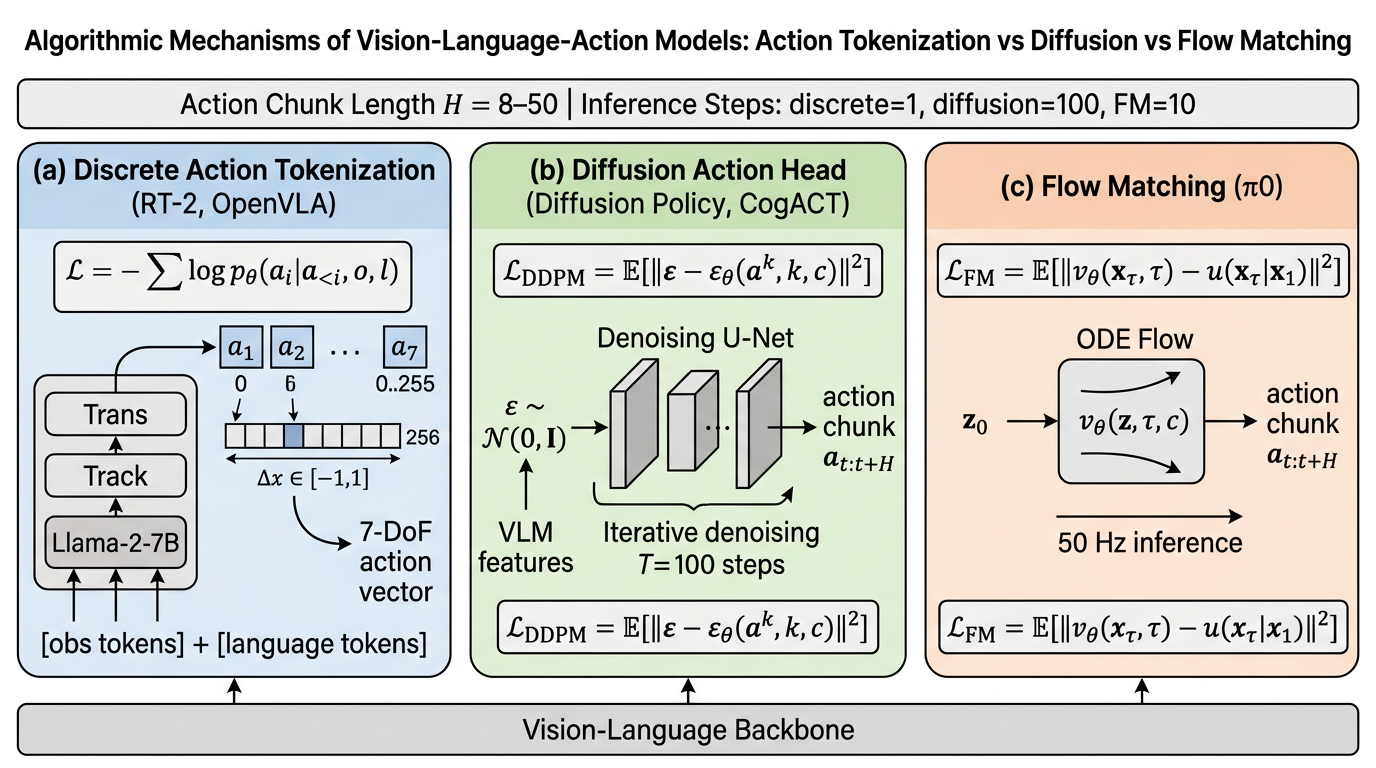
\includegraphics[keepaspectratio,alt={Algorithmic mechanism schematic of three VLA action heads: discrete tokens, diffusion, flow matching}]{./figures/Vision-Language-Action-Models__vla_algorithms.png}}
\caption{Algorithmic mechanism schematic of three VLA action heads: discrete tokens, diffusion, flow matching}
\end{figure}

\subsection{Visual Encoders and Spatial Tokenization (SigLIP, DINOv2, 3D Lifting)}\label{visual-encoders-and-spatial-tokenization-siglip-dinov2-3d-lifting}

This subsection reviews the visual front-ends that feed VLA backbones, organized as 2D encoders, 3D-lifting variants, and tokenization economics. A VLA's perception stack is almost always built from a frozen or partially fine-tuned visual encoder. The encoder produces a sequence of patch tokens for the language backbone to attend over. Three encoder families dominate. \textbf{SigLIP} is a sigmoid-loss CLIP variant. It supplies semantic, language-aligned features at 384²--768² resolution. SigLIP is the primary encoder in OpenVLA and many derivatives. \textbf{DINOv2} supplies spatial-rich self-supervised features that complement SigLIP. OpenVLA concatenates the two and gains \textasciitilde6\% absolute on real-robot generalization splits relative to SigLIP-only. \textbf{Qwen2-VL's native ViT} integrates dynamic-resolution tokenization. It retains absolute coordinates of patches and enables SpatialVLA's superior performance on spatially-precise tasks.

Representative visual-encoder methods include: CLIP (2021, contrastive image-text alignment at 400M-pair scale), ALIGN (2021, billion-scale noisy alignment), SigLIP (2023, sigmoid-loss replacement that scales to larger batches), DINOv2 (2023, self-supervised ViT capturing dense spatial features), Qwen2-VL ViT (2024, dynamic-resolution patch tokenizer with absolute coordinates), PaliGemma's SigLIP-So400m (2024, 400M parameters fine-tuned on multimodal mixtures), InternVL-V (2024, 6B vision encoder for high-resolution input), RVT-2 (2024, multi-view re-rendering for high-precision insertion), RISE (2024, 3D point-cloud transformer for camera-invariant policies), and SpatialVLA's 3D ego-token encoder (2025, robot-centric Cartesian tokenization).

Beyond 2D, three lines of work add 3D structure. \textbf{RVT-2} {[}Goyal et al., 2024{]} re-renders the scene from multiple virtual cameras and feeds the synthesized views to a transformer, achieving high-precision insertions (8 mm peg, 16 mm peg) from few demonstrations. \textbf{RISE} {[}Wang et al., 2024{]} lifts the encoder to a 3D point-cloud transformer for camera-invariant policies. \textbf{SpatialVLA} {[}Qu et al., 2025{]} tokenizes ego-centric 3D coordinates so that the VLM directly reasons about object positions in robot-centric Cartesian space. The empirical pattern across all three: 3D structure helps most on contact-rich, occlusion-heavy, and viewpoint-shifted tasks, with diminishing returns on free-space pick-and-place.

A practical detail: the number of patch tokens per frame, \(N_v\), is the dominant cost driver of monolithic VLA inference. OpenVLA uses 256 tokens per camera at 224² resolution; SpatialVLA uses up to 1024 with adaptive resolution. Each extra patch token costs \(O(N_v \cdot d)\) in attention, so reducing \(N_v\) via token merging (ToMe) or pooling is a main lever in efficient-VLA work such as BLURR {[}Ma et al., 2025{]} and DySL-VLA {[}Yang et al., 2026{]}.

\subsection{Action Tokenization Schemes (RT-2 256-bin, FAST, Continuous Embeddings)}\label{action-tokenization-schemes-rt-2-256-bin-fast-continuous-embeddings}

Building on the visual front-end of §4.1, this subsection examines how the resulting feature stream is mapped to executable actions. The action representation is the single design choice that most distinguishes VLA from other multimodal architectures. It determines how a generative \emph{language} model ends up emitting a \emph{control} signal. Three regimes coexist.

Representative action-tokenization methods include: RT-1 (2022, 11-token discrete encoding with separate gripper and termination heads), RT-2 (2023, 256-bin per-dimension quantile-binned discrete tokens reusing rare LLM vocabulary entries), OpenVLA (2024, identical 256-bin scheme on Llama-2-7B), FAST (2024, frequency-aware DCT-compressed action chunks tokenized to 8--16 tokens), OpenVLA-Pro (2025, FAST tokens with 5× decode speedup), OpenVLA-OFT (2025, parallel decoding of all 7 dimensions with continuous head), Octo-small (2024, single-step MLP regression at 25--50 Hz), Diffusion Policy (2023, action-chunk denoising via DDPM), CogACT (2024, Diffusion Transformer over chunked actions), π0 (2024, conditional flow matching at 50 Hz), and ACT (2023, action-chunking VAE for ALOHA bimanual control).

The original \textbf{RT-2 / OpenVLA scheme} discretizes each of the 7 (or 14) action dimensions into 256 bins using a per-dimension quantile transform, then maps each bin to a token taken from the LLM's least-used vocabulary entries. With \(K = 256\) bins, the per-dimension entropy upper bound is 8 bits, and 7 action dimensions consume 56 bits per timestep --- a manageable autoregressive overhead. The cross-entropy training loss is identical to standard language modeling. The advantage is full reuse of LLM machinery; the disadvantage is the quantization floor: 0.0078 absolute precision on a normalized {[}-1,1{]} axis is borderline for sub-mm tasks.

\textbf{FAST tokenizer} (Frequency-Aware Action Sequence Tokenizer, used in OpenVLA-Pro and X-VLA derivatives) replaces uniform binning with discrete cosine transform compression of action chunks, then quantizes coefficients. Because most of the variance in human-collected demonstrations lives in low-frequency components, FAST compresses 30--50-step action chunks into 8--16 discrete tokens with negligible reconstruction loss, dramatically reducing decode latency.

\textbf{Continuous embeddings} project the last hidden state through a small MLP to produce real-valued actions directly. OpenVLA-OFT, Octo's small variants, and CogACT's reflex head use this. The natural loss is MSE, but MSE collapses on multimodal demonstrations; in practice continuous heads are paired with a chunk-level tokenizer (action chunking transformer, ACT) or with diffusion to recover multi-modality.

\subsection{Training Losses: Cross-Entropy, MSE, Diffusion DDPM, Flow Matching, ECoT Auxiliary}\label{training-losses-cross-entropy-mse-diffusion-ddpm-flow-matching-ecot-auxiliary}

Whereas §4.2 fixed the action representation, this subsection turns to the loss that drives the parameter update. Five training losses cover the literature.

Representative training-objective methods include: RT-2 (2023, autoregressive cross-entropy on 256-bin tokens with web-VQA co-finetuning), OpenVLA (2024, cross-entropy on Llama-2 vocabulary slots), Octo-small (2024, MSE regression on continuous chunks), Diffusion Policy (2023, DDPM denoising loss with EDM noise schedule), CogACT (2024, Diffusion Transformer with classifier-free guidance), π0 (2024, conditional flow matching with straight-line interpolation), π0.5 (2025, CFM plus cross-embodiment co-training), ECoT (2024, chain-of-thought cross-entropy auxiliary on plan/subtask/gripper/motion tokens), V-GPS (2024, Q-value regression via offline RL), CLIP-RT (2025, contrastive language-action distillation), and Discrete Policy (2024, disentangled action-space cross-entropy across multitask heads).

\textbf{Cross-entropy} (RT-2, OpenVLA): \(\mathcal{L}_{\text{CE}} = -\sum_{i} \log p_\theta(a_i \mid a_{<i}, o, l)\), summed across the 7 action tokens; in co-finetuning runs, an additional language-modeling loss on web text preserves semantic priors and prevents catastrophic forgetting.

\textbf{MSE / L1 regression} (Octo-small, OpenVLA-OFT continuous head): \(\mathcal{L}_{\text{MSE}} = \|\hat{a} - a\|_2^2\). Simple but mode-averaging.

\textbf{DDPM denoising} (Diffusion Policy, CogACT, Octo-large): \(\mathcal{L}_{\text{DDPM}} = \mathbb{E}_{k, \varepsilon}\big[\|\varepsilon - \varepsilon_\theta(a^k, k, c)\|^2\big]\) where \(a^k\) is the noised action chunk at diffusion step \(k\), \(c\) is the conditioning (VLM features, optional language), and \(\varepsilon \sim \mathcal{N}(0, I)\). The number of diffusion steps \(T\) is typically 100 at training, distilled to 1--8 at inference via Consistency Policy {[}Prasad et al., 2024{]}.

\textbf{Conditional flow matching} (π0, π0.5): \(\mathcal{L}_{\text{CFM}} = \mathbb{E}_{\tau, x_1, x_\tau}\big[\|v_\theta(x_\tau, \tau, c) - u(x_\tau \mid x_1)\|^2\big]\) where \(u(x_\tau \mid x_1) = x_1 - x_0\) is the conditional vector field along a straight-line interpolation from noise \(x_0\) to data \(x_1\). CFM is empirically more stable to train than DDPM and admits 5-step Euler integration at inference.

\textbf{Auxiliary losses} include the \textbf{ECoT} chain-of-thought cross-entropy (Zawalski et al., 2024), Q-value regression for \textbf{V-GPS} {[}Nakamoto et al., 2024{]}, and contrastive language-action losses for \textbf{CLIP-RT} {[}Kang et al., 2025{]}. Auxiliary losses typically help out-of-distribution generalization but cost additional compute at training time only --- a favorable trade.

\subsection{Inference Acceleration: Action Chunking, KV-Cache, Layer Skipping (DySL-VLA), BLURR}\label{inference-acceleration-action-chunking-kv-cache-layer-skipping-dysl-vla-blurr}

This subsection reviews engineering techniques that close the gap between VLM training latency and robot control frequency. Inference latency is the critical engineering constraint for deploying VLAs on robots. Five techniques combine to bridge the gap from VLM-native \textasciitilde5 Hz to robot-required 50--200 Hz.

Representative inference-acceleration methods include: ACT (2023, action chunking with H=100 on ALOHA bimanual), RT-2 (2023, KV-cache reuse for vision tokens), OpenVLA (2024, vision-token caching across chunk windows), OpenVLA-OFT (2025, parallel decoding of 7 action tokens cutting decode latency by 6×), π0 (2024, action chunking with H=50 amortizing one VLM pass over 1 s), π0.5 (2025, overlapping chunks with 0.2 s replanning), TinyVLA (2024, sub-billion-parameter distilled student), MiniVLA (2024, 1B-parameter distillation retaining \textasciitilde85\% of OpenVLA-7B), BLURR (2025, INT4 quantization plus KV compression plus layer skipping for \textasciitilde4× speedup), DySL-VLA (2026, dynamic-static layer skipping for 2--3× speedup), Consistency Policy (2024, diffusion distillation to 1--8 inference steps), and Mixture-of-Expert Denoisers (2024, MoE diffusion experts for multitask amortization).

\textbf{Action chunking} {[}Zhao et al., 2023; Black et al., 2024{]} predicts \(H\) future actions per forward pass and executes them open-loop or with re-planning every \(K \le H\) steps. Action Chunking Transformer (ACT) used \(H=100\) on ALOHA bimanual tasks. π0 uses \(H = 50\) at 50 Hz, so a single VLM forward pass amortizes over 1 second of motion. The cost is that closed-loop reactivity drops; π0.5 mitigates this with overlapping chunks and re-planning every 0.2 s.

\textbf{Parallel decoding for discrete heads} (OpenVLA-OFT) decodes all 7 action tokens in parallel rather than autoregressively, cutting decode latency by \textasciitilde6× because the action tokens have no causal dependency for a single timestep.

\textbf{KV-cache reuse} retains the keys/values for visual and instruction tokens across multiple action chunks, since those tokens do not change. This eliminates the dominant compute cost (vision-token attention) for all but the first inference per chunk window.

\textbf{Layer skipping} (DySL-VLA {[}Yang et al., 2026{]}) dynamically skips transformer layers that contribute little to action prediction, achieving 2--3× speedup with minimal accuracy loss. \textbf{BLURR} {[}Ma et al., 2025{]} proposes a boosted low-resource inference stack that combines INT4/INT8 quantization, KV-cache compression, and layer skipping, fitting OpenVLA-7B on commodity 12 GB GPUs at \textgreater20 Hz.

\textbf{Distillation} to smaller VLAs (TinyVLA, MiniVLA) is the heaviest hammer, trading capability for latency. Empirically, MiniVLA at 1B parameters retains \textasciitilde85\% of OpenVLA-7B's success rate on LIBERO at 4× the throughput.

{\def\LTcaptype{none} % do not increment counter
\begin{longtable}[]{@{}
  >{\raggedright\arraybackslash}p{(\linewidth - 8\tabcolsep) * \real{0.2697}}
  >{\raggedright\arraybackslash}p{(\linewidth - 8\tabcolsep) * \real{0.1348}}
  >{\raggedleft\arraybackslash}p{(\linewidth - 8\tabcolsep) * \real{0.2584}}
  >{\raggedright\arraybackslash}p{(\linewidth - 8\tabcolsep) * \real{0.1461}}
  >{\raggedright\arraybackslash}p{(\linewidth - 8\tabcolsep) * \real{0.1910}}@{}}
\toprule\noalign{}
\begin{minipage}[b]{\linewidth}\raggedright
Technique
\end{minipage} & \begin{minipage}[b]{\linewidth}\raggedright
Model Mod.
\end{minipage} & \begin{minipage}[b]{\linewidth}\raggedleft
Typical Speedup
\end{minipage} & \begin{minipage}[b]{\linewidth}\raggedright
Accuracy Cost
\end{minipage} & \begin{minipage}[b]{\linewidth}\raggedright
First Reported
\end{minipage} \\
\midrule\noalign{}
\endhead
\bottomrule\noalign{}
\endlastfoot
Action chunking (H=8--50) & architecture & 8--50× & small & ACT 2023, π0 2024 \\
Parallel decoding & head & 6× & minimal & OpenVLA-OFT 2025 \\
KV-cache reuse & runtime & 3--5× & none & OpenVLA 2024 \\
Layer skipping (DySL) & architecture & 2--3× & \textless2\% SR & DySL-VLA 2026 \\
INT4 quantization & weights & 2--3× memory; 1.5× speed & 1--4\% SR & BLURR 2025 \\
Distillation to \textless1B & full & 4--6× & 5--15\% SR & TinyVLA 2024 \\
\end{longtable}
}

\textbf{Table 5.} Inference acceleration techniques, type of modification, typical speedup, accuracy impact, and origin.

A unifying observation is that the design space is not ``pick one technique'' but ``stack them carefully.'' The current state-of-the-art deployment recipe --- exemplified by π0.5 and Helix --- combines action chunking (\(H = 25\)), KV-cache reuse, and a distinct fast reflex head, achieving 50 Hz dexterous control with a 3-billion-parameter brain. By 2026, BLURR-style INT4 inference and dynamic layer skipping are the additional compute optimizations that bring 7B-class VLAs onto edge GPUs. Looking forward, two further levers remain: speculative decoding for action tokens (analogous to NLP speculative decoding) and learned routers in MoE-style VLAs (X-VLA), both of which are active research areas.

A final algorithmic note concerns the training pipeline as a whole, not just losses. Modern VLA training proceeds in three stages: (i) load a pretrained VLM checkpoint (PaLI, Llama-2, PaliGemma); (ii) ``warm'' finetune on a large robot mixture (OXE, in-house data) with the action head attached, often with a low learning rate (1e-5 to 5e-5) on the backbone and a higher rate (1e-4) on new parameters; (iii) optionally fine-tune on a target embodiment with a small dataset (10--500 episodes). OpenVLA used 64 A100s for \textasciitilde2 weeks at stage (ii); π0 used a substantially larger compute budget that has not been fully disclosed; Gemini Robotics 1.5 reportedly trained on TPU v5p pods, though numbers remain proprietary. Stage (iii) is now standard practice for any deployed VLA --- it is the equivalent of NLP ``instruction tuning'' and reliably yields 10--40\% absolute success-rate gains on the target embodiment over zero-shot evaluation {[}Kim et al., 2024; Black et al., 2024; Barreiros et al., 2026{]}.

\section{Datasets, Embodiments, and the Open X-Embodiment Pretraining Corpus}\label{datasets-embodiments-and-the-open-x-embodiment-pretraining-corpus}

Whereas §4 showed that algorithmic choices buy 5--55 percentage points of success rate, this section turns to the data underneath, which buys an order of magnitude more. The dataset landscape is the single most consequential factor in VLA progress. Robot-data scaling, not parameter scaling alone, gates generalization. Ai et al.'s {[}2025{]} embodiment scaling laws empirically confirm this. The corpora that recur throughout the survey have specific sizes worth memorizing. RT-1 contains 130k episodes across 13 EDR robots, 700+ skills, and a 17-month collection. BridgeData V2 contains \textasciitilde60k demonstrations on WidowX 250s, 24 environments, and 13 skills. RH20T contains 110k trajectories across 147 tasks with multi-modal sensing. ALOHA is a 50 Hz bimanual platform with 14 dexterous tasks at sub-\$20k hardware cost. Mobile ALOHA adds 50 hours of teleoperated cooking and cleaning. RoboMIND contains 107k trajectories across 4 embodiments, 479 tasks, and 96 objects. DROID contains 76k trajectories at 350 hours across 564 scenes and 86 tasks, collected by 50 collectors at 13 institutions on identical Franka Pandas. The Open X-Embodiment (OXE) collaboration aggregates 22 embodiments, 311 scenes, 527 skills, and \textasciitilde1M trajectories in RLDS format. Internet video (Ego4D's 3,670 hours, EpicKitchens, EgoExo4D), synthetic augmentation (ROSIE, OXE-AugE), and retargeted human demonstrations (X-Diffusion) extend the data frontier beyond curated teleoperation. The recurring failure modes in this layer are also concrete: license fragmentation across OXE, schema drift between v6 and v9, and a sim-to-real gap that simulators such as SimplerEnv calibrate to within ±5\%. The rest of this section walks through these corpora in order of role: curated robot datasets (§5.1), the OXE federation (§5.2), and in-the-wild long-tail sources (§5.3).

\subsection{Curated Robot Datasets: RT-1, BridgeData V2, RH20T, ALOHA, RoboMIND}\label{curated-robot-datasets-rt-1-bridgedata-v2-rh20t-aloha-robomind}

This subsection catalogues the curated single-lab datasets that remain canonical fine-tuning resources, organized by year and embodiment. The pre-OXE era produced several individual datasets that remain canonical fine-tuning resources today.

Representative curated robot datasets include: RT-1 (2022, 130k episodes across 13 EDR robots over 17 months), BridgeData (2021, \textasciitilde7k tasks on a single WidowX), BridgeData V2 (2023, \textasciitilde60k demonstrations across 24 environments and 13 skills on WidowX 250s), RH20T (2023, 110k demonstrations across 147 tasks with audio and tactile streams), ALOHA (2023, 50 Hz bimanual platform under \$20k with 14 dexterous tasks), Mobile ALOHA (2024, 50 hours teleoperated cooking and cleaning on a wheeled bimanual base), RoboMIND (2024, 107k trajectories across 4 embodiments and 479 tasks with 96 objects), DROID (2024, 76k trajectories at 350 hours across 564 scenes on identical Franka Pandas), TACO-RL (2023, language-relabeled tabletop demonstrations), Bridge-Robotic-Library (2024, multi-camera Franka demonstrations), and Mosaic (2024, mixed-quality demonstrations with success annotations). \textbf{RT-1 dataset} {[}Brohan et al., 2023{]} comprises 130,000 episodes collected over 17 months across 13 EDR robots in Google's office kitchens, covering 700+ skill instances spanning pick, place, drawer manipulation, knock, slide, and re-orient verbs. Each episode carries a natural-language instruction, third-person and wrist-camera RGB at 256×320, and 7-DoF Cartesian end-effector deltas at 3 Hz. RT-1 is the largest single-robot demonstration corpus published before OXE.

\textbf{BridgeData V2} {[}Walke et al., 2023{]} contains roughly 60,000 demonstrations across 24 environments and 13 skills on a WidowX 250s arm. It was specifically designed for cross-task and cross-environment generalization studies and is the de-facto benchmark fine-tuning split for OpenVLA. \textbf{RH20T} {[}Fang et al., 2023{]} adds 110,000 demonstrations across 147 manipulation tasks with multi-modal sensing including audio and tactile streams.

\textbf{ALOHA} {[}Zhao et al., 2023{]} introduced a low-cost (\(<\)\$20k) bimanual platform with two 6-DoF Trossen arms and synchronized teleoperation; the public ALOHA dataset spans tasks like cup stacking, candy unwrapping, and battery insertion at 50 Hz, 480p RGB. \textbf{Mobile ALOHA} {[}Fu et al., 2024{]} extends to a wheeled base supporting whole-body bimanual manipulation; its release dataset includes 50 hours of teleoperated cooking, cleaning, and elevator interaction.

\textbf{RoboMIND} {[}Wu et al., 2024{]} is the largest recent multi-embodiment academic dataset, containing 107k demonstration trajectories across 479 diverse tasks involving 96 objects on 4 embodiments (Franka, UR5, AgileX, humanoid). RoboMIND was specifically curated to test cross-embodiment fine-tuning and is the dominant Chinese-lab fine-tuning corpus.

\textbf{DROID} {[}Khazatsky et al., 2024{]} is the largest in-the-wild dataset to date: 76,000 demonstration trajectories totalling 350 hours, 564 distinct scenes spanning 86 university and industrial environments collected by 50 data collectors at 13 institutions on identical Franka Panda hardware over 12 months. DROID's contribution is \emph{scene diversity}: where RT-1 was 13 robots in a few kitchens, DROID is one robot in 564 environments, enabling controlled studies of perceptual generalization.

\subsection{Open X-Embodiment: Composition, Embodiments, and Mixture Strategies}\label{open-x-embodiment-composition-embodiments-and-mixture-strategies}

Whereas §5.1 surveyed individual lab datasets, this subsection turns to the federated OXE corpus that unifies them. The \textbf{Open X-Embodiment (OXE) Collaboration} {[}O'Neill et al., 2023{]} aggregated 21 institutions' robot datasets into a unified RLDS-format corpus. As of the v9 release the corpus contains 22 distinct embodiments (Franka Panda, WidowX, UR5, xArm, Sawyer, Jaco, Kuka, Google Robot, etc.), 311 scenes, 527 skills, and over 1 million trajectories. Action spaces are normalized into a 7-DoF schema with embodiment-specific tokens; observations are resized to 224×224. The collaboration also released \textbf{RT-1-X} and \textbf{RT-2-X}, models trained on the full OXE mixture, and demonstrated that an OXE-trained policy outperforms each lab's local model on its \emph{own} held-out evaluation by an average of 50\% --- direct evidence that cross-embodiment positive transfer is real and large.

Mixture strategies for OXE training are an active research topic. The original RT-X paper used uniform sampling across datasets; OpenVLA used a frequency-weighted sampler that down-weights large datasets to prevent BridgeData from dominating; π0 used a curriculum that begins with simple single-arm data and adds bimanual data later; X-VLA introduced soft prompts to embed embodiment identity. The general empirical finding is that \emph{embodiment count matters more than per-robot data size}: Ai et al.'s {[}2025{]} embodiment scaling laws show that adding the 22nd embodiment helps more than doubling the data of the largest one, motivating continued community contribution.

\subsection{In-the-Wild and Long-Tail Sources: DROID, Internet Video, Egocentric Human Videos}\label{in-the-wild-and-long-tail-sources-droid-internet-video-egocentric-human-videos}

Building on the curated and federated corpora of §§5.1--5.2, this subsection examines long-tail data that extends the frontier beyond teleoperation. Beyond curated robot datasets, three wider data sources are increasingly leveraged.

Representative long-tail data sources include: DROID (2024, 76k Franka trajectories across 564 scenes), Ego4D (2022, 3,670 hours of egocentric human video), EpicKitchens (2018--2023, multi-day kitchen recordings), EgoExo4D (2024, paired ego-exo human demonstrations), Something-Something-V2 (2017, fine-grained action understanding), HowTo100M (2019, instructional internet video), ROSIE (2023, image-editing diffusion synthesizing novel scenes from real demos), OXE-AugE (2025, image-editing augmentation generating 4× expanded OXE corpus), X-Diffusion (2025, retargeted human hand demonstrations via differentiable kinematics), Open-TeleVision (2024, low-cost VR teleoperation collection), RoboCasa-1k (2024, simulated household-scale demonstrations across 100+ kitchens), and Habitat-3.0 (2024, simulated mobile-manipulation episodes). \textbf{Internet video} {[}McCarthy et al., 2025 survey{]} --- YouTube cooking videos, Ego4D, EpicKitchens --- supplies trillions of frames of human manipulation but lacks action labels. The standard recipe is to (a) extract pseudo-actions via inverse-dynamics models, (b) co-train a VLA on real-robot data and pseudo-labeled video, or (c) use video as a perception-only pretraining signal. \textbf{X-Diffusion} {[}Pace et al., 2025{]} trained diffusion policies on cross-embodiment human demonstrations, retargeting human hand trajectories onto robot end-effectors via differentiable kinematics.

\textbf{Egocentric human videos} (Ego4D, ARIA datasets, EgoExo4D) are particularly valuable because they share viewpoint with wrist-mounted robot cameras. RoboCat-style co-training uses egocentric human episodes as additional pretraining; ablations show that 1 hour of egocentric video provides roughly the same generalization benefit as 30 minutes of real robot teleoperation, a 30:1 sample-efficiency multiplier.

\textbf{Sim-to-real synthetic data} rounds out the picture. RoboCasa, Habitat 3.0, and ManiSkill3 generate millions of simulated trajectories cheaply, but the sim-to-real gap remains significant for contact-rich tasks. \textbf{Scaling Robot Learning with Semantically Imagined Experience (ROSIE)} {[}Yu et al., 2023{]} used image-editing diffusion models to \emph{synthesize} novel scenes from real demonstrations, expanding effective scene diversity without new physical collection. \textbf{OXE-AugE} {[}Ji et al., 2025{]} extends this by augmenting OXE itself with synthesized robot images, producing a 4× expanded corpus with measurable cross-embodiment transfer gains.

{\def\LTcaptype{none} % do not increment counter
\begin{longtable}[]{@{}
  >{\raggedright\arraybackslash}p{(\linewidth - 10\tabcolsep) * \real{0.1604}}
  >{\raggedright\arraybackslash}p{(\linewidth - 10\tabcolsep) * \real{0.0377}}
  >{\raggedleft\arraybackslash}p{(\linewidth - 10\tabcolsep) * \real{0.1415}}
  >{\raggedleft\arraybackslash}p{(\linewidth - 10\tabcolsep) * \real{0.1792}}
  >{\raggedright\arraybackslash}p{(\linewidth - 10\tabcolsep) * \real{0.2547}}
  >{\raggedright\arraybackslash}p{(\linewidth - 10\tabcolsep) * \real{0.2264}}@{}}
\toprule\noalign{}
\begin{minipage}[b]{\linewidth}\raggedright
Dataset
\end{minipage} & \begin{minipage}[b]{\linewidth}\raggedright
Year
\end{minipage} & \begin{minipage}[b]{\linewidth}\raggedleft
Trajectories
\end{minipage} & \begin{minipage}[b]{\linewidth}\raggedleft
Embodiments
\end{minipage} & \begin{minipage}[b]{\linewidth}\raggedright
Scenes / Tasks
\end{minipage} & \begin{minipage}[b]{\linewidth}\raggedright
Key Use
\end{minipage} \\
\midrule\noalign{}
\endhead
\bottomrule\noalign{}
\endlastfoot
RT-1 & 2022 & 130,000 & 13 (EDR) & 700+ tasks & Single-robot pretraining \\
BridgeData V2 & 2023 & 60,000+ & 1 (WidowX) & 24 environments / 13 skills & Cross-task evaluation \\
RH20T & 2023 & 110,000 & several & 147 tasks & Multi-modal demos \\
ALOHA & 2023 & \textasciitilde10 hr per task & 1 (bimanual) & 14 dexterous tasks & Bimanual fine-tuning \\
Mobile ALOHA & 2024 & 50 hr & 1 (mobile bimanual) & 7 mobile tasks & Whole-body manipulation \\
RoboMIND & 2024 & 107,000 & 4 & 479 tasks / 96 objects & Multi-embodiment \\
Open X-Embodiment & 2023 & 1M+ & 22 & 311 scenes / 527 skills & Generalist pretraining \\
DROID & 2024 & 76,000 & 1 (Franka) & 564 scenes / 86 tasks & Scene diversity \\
Ego4D & 2022 & 3,670 hr & --- (humans) & 9 scenarios / 74 locations & Human-video pretraining \\
ROSIE-augmented & 2023 & synthesized & varies & augmented scenes & Synthetic augmentation \\
\end{longtable}
}

\textbf{Table 6.} Major datasets used in vision-language-action research, with approximate sizes, embodiment count, scope, and primary use.

The dataset story has three implications that recur in later sections. First, the OXE corpus is the \emph{de facto} pretraining substrate for any open-weight VLA in 2024--2026; all major open releases (OpenVLA, Octo, CogACT, SpatialVLA, X-VLA) train on OXE or a near-superset. Second, fine-tuning on a target embodiment with 100--500 in-domain demonstrations is the standard last-mile recipe and is responsible for most reported real-world gains. Third, the long tail --- humans, simulation, internet video --- is increasingly important not as a replacement for real teleoperation but as a \emph{generalization regularizer}; this is the primary frontier of dataset research in 2026. We expect by 2027 that the largest VLA pretraining mixture will be 30\% real teleoperation, 30\% retargeted human video, 30\% synthetic, and 10\% paired captioned web image-text --- a substantial shift from the 95\%-real RT-2 era.

A final practical point on data licensing: OXE includes datasets with mixed licenses (CC-BY, custom academic, internal Google with redistribution), and OpenVLA's release explicitly carved out a Bridge-V2-like subset that is permissively licensed. This bifurcation is unlikely to disappear soon, and any future industrial VLA stack will need careful license bookkeeping. The community is converging on a small set of ``clean'' datasets --- DROID, BridgeData V2, RoboMIND, and the OXE permissive subset --- for academic experiments, with industrial systems supplementing privately.

\section{Benchmarks, Evaluation Protocols, and Metrics for Vision-Language-Action Models}\label{benchmarks-evaluation-protocols-and-metrics-for-vision-language-action-models}

Whereas §5 catalogued what we train on, this section catalogues what we report. VLA evaluation has matured rapidly between 2022 and 2026. Reporting moved from per-paper real-world demos with 10--20 trials to standardized simulators, distributed real-world services, and stress-test protocols. Standardized simulators include CALVIN (4 environments, 5-step chains), LIBERO (130 task suites, five distribution-shift splits), SimplerEnv (calibrated Gazebo replicas of Google Robot and WidowX), ManipBench (10k+ low-level prompts), and LoHoRavens (50-step horizons). Distributed real-world services include AutoEval (10 robot-days at 6 institutions, {[}Zhou et al., 2025{]}) and RoboArena (50--100 trials per cell with bootstrap confidence intervals across institutional Frankas, {[}Atreya et al., 2025{]}). Stress-test protocols include AGENTSAFE (200+ hazardous prompts), Tong et al.~(200+ paraphrasings), Hou et al.~(5 cm positional shifts), and EmbodiedGovBench (governance/recovery suites). The headline mid-2026 numbers worth memorizing are concrete. OpenVLA reaches 76.5\% LIBERO and 64\% RoboArena. OpenVLA-OFT reaches 87.4\% LIBERO-90 at 25 Hz and 73\% RoboArena. CogACT reaches 91.4\% LIBERO and +55\% real over OpenVLA. π0 reaches 83.9\% zero-shot and 96.5\% fine-tuned LIBERO with 71\% / 88\% on RoboArena. Octo-large reaches 51\% RoboArena. Common failure modes that benchmarks now expose include linguistic fragility (--18 pp under paraphrase), positional brittleness (--25 to --35 pp beyond 5 cm shift), 30--50\% baseline compliance with hazardous instructions, and 15--30 pp drops under lighting changes. Figure 5 maps fifteen benchmarks against two crucial axes --- task horizon and generalization stress --- to show the design space. This section walks the principal benchmarks, their protocols, and the metrics that researchers and reviewers use to compare systems.

\begin{figure}
\centering
\pandocbounded{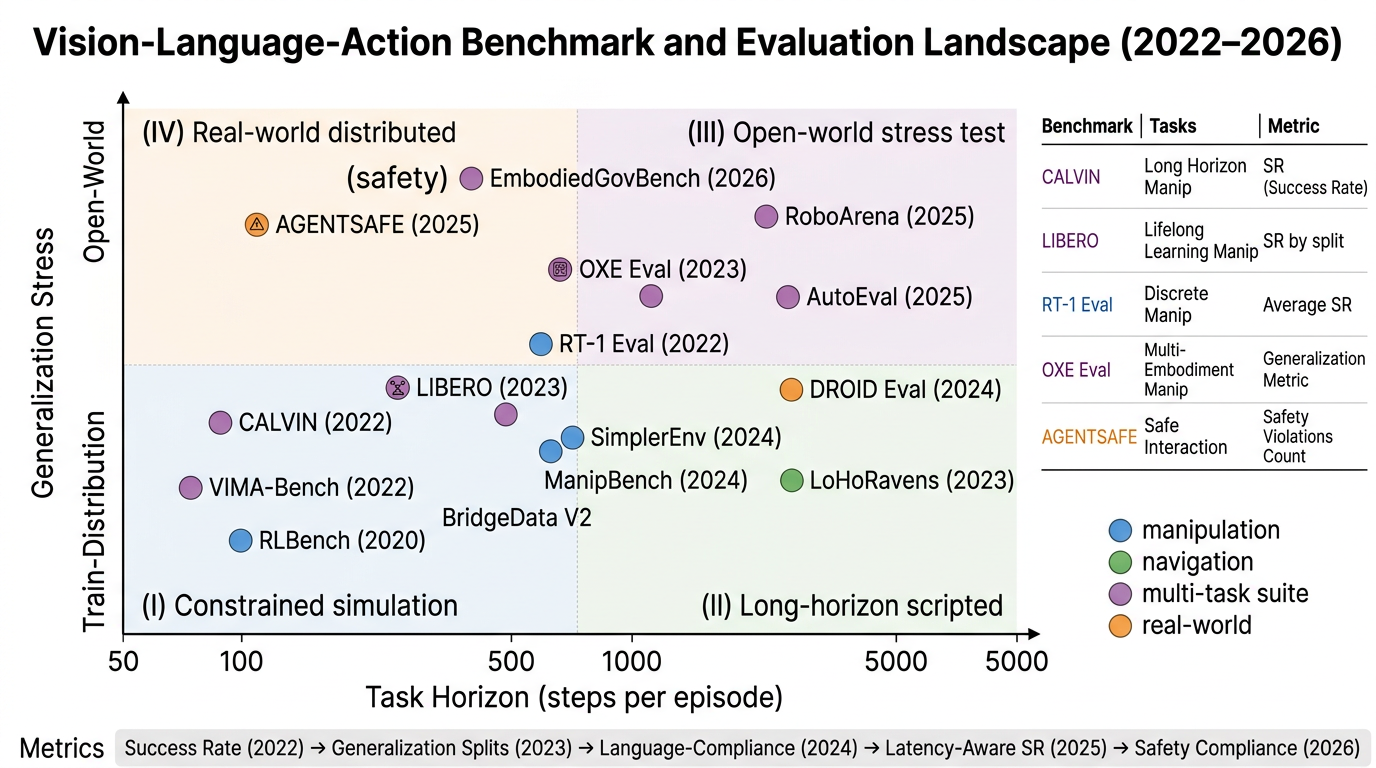
\includegraphics[keepaspectratio,alt={Benchmark and evaluation landscape for vision-language-action models}]{./figures/Vision-Language-Action-Models__vla_benchmarks.png}}
\caption{Benchmark and evaluation landscape for vision-language-action models}
\end{figure}

\subsection{Simulation Benchmarks: CALVIN, LIBERO, SimplerEnv, ManipBench, LoHoRavens}\label{simulation-benchmarks-calvin-libero-simplerenv-manipbench-lohoravens}

This subsection reviews simulation benchmarks ordered by horizon length and generalization stress. Simulation provides cheap, reproducible evaluation but cannot fully validate physical-contact behavior.

Representative simulation benchmarks include: RLBench (2020, 100 tasks in CoppeliaSim with Franka), CALVIN (2022, 4 environments A/B/C/D with 5-step language chains), LIBERO (2023, 130 tasks across 5 distribution-shift splits in MuJoCo), VIMA-Bench (2022, 17 tasks with multimodal interleaved prompts on UR5), LoHoRavens (2023, 12 long-horizon tabletop tasks with up to 50 sub-steps), SimplerEnv (2024, calibrated Gazebo replicas of Google Robot and WidowX within ±5\% of real), ManipBench (2025, 10,000+ low-level manipulation prompts for VLM evaluation), RoboCasa (2024, 100+ simulated kitchen tasks for mobile manipulation), Habitat-Manipulation (2024, mobile manipulation in photorealistic homes), GENESIS (2024, GPU-accelerated physics for RL pretraining), ARNOLD (2024, language-grounded continuous control), and ManiSkill3 (2024, contact-rich manipulation with 30+ tasks).

\textbf{CALVIN} {[}Mees et al., 2022{]} is the canonical simulation benchmark for language-conditioned long-horizon manipulation. Built in PyBullet, CALVIN ships four environments labeled A/B/C/D with varying lighting, table textures, and object configurations, and provides 24 hours of teleoperated play data with crowdsourced language annotations. The standard protocol asks a policy to complete a chain of 5 sub-tasks specified in natural language, scoring the longest contiguous prefix of correctly executed sub-tasks (``CALVIN average length''). Strong VLAs reach 4.0+ out of 5.0 in 2026, up from RT-1's 1.0 in 2022.

\textbf{LIBERO} {[}Liu et al., 2023{]} is the second pillar, targeting generalization explicitly. LIBERO splits 130 task suites into five distribution-shift categories: LIBERO-Spatial, LIBERO-Object, LIBERO-Goal, LIBERO-90 (multitask), and LIBERO-Long (long-horizon). Each task provides \textasciitilde50 demonstrations and a templated language instruction. Reported success rates as of mid-2026: OpenVLA averages 76.5\%; OpenVLA-OFT 87.4\%; CogACT 91.4\%; π0 (zero-shot) 83.9\%; π0 (fine-tuned) 96.5\% (matching state-of-the-art among open VLAs). The LIBERO suite has become the \emph{MNIST} of VLA --- too small to be conclusive, but the universal first stop.

\textbf{SimplerEnv} {[}Li et al., 2024{]} addresses the ``simulation is unrepresentative'' critique by carefully calibrating a Gazebo-based replica of the Google Robot and WidowX environments used by RT-1/RT-2/OpenVLA. SimplerEnv reports reproducible numbers within ±5\% of real-world success rates for OpenVLA and Octo, a substantial improvement over earlier, miscalibrated simulators. \textbf{ManipBench} {[}Zhao et al., 2025{]} benchmarks low-level manipulation reasoning of VLMs across 10,000+ low-level prompts, exposing a strong gap between VLM commonsense and VLA control. \textbf{LoHoRavens} {[}Zhang et al., 2023{]} specializes in long-horizon language-conditioned tabletop tasks with up to 50 sub-steps, where most VLAs degrade ungracefully.

\textbf{RoboCasa} simulates household-scale environments with 100+ kitchens; \textbf{VIMA-Bench} evaluates multimodal-prompt manipulation with interleaved image-text inputs; \textbf{RLBench} remains a useful fine-motor benchmark for low-level policies but lacks the language richness of CALVIN/LIBERO.

\subsection{Real-World Evaluation: RoboArena, AutoEval, DROID Eval Splits}\label{real-world-evaluation-roboarena-autoeval-droid-eval-splits}

Whereas §6.1 covered simulators, this subsection turns to physical-world evaluation services that produce reproducible cross-lab leaderboards. Simulation alone cannot validate physical-contact policies. Real-world evaluation has historically been irreproducible because each lab uses unique hardware.

Representative real-world evaluation infrastructures include: AutoEval (2025, autonomous robot self-evaluation across 6 institutions over 10 robot-days), RoboArena (2025, distributed Franka leaderboard with 50--100 trials per cell and bootstrap CIs), DROID Eval (2024, 564-scene held-out language-conditioned split), BridgeData V2 Eval (2023, WidowX 13-skill × 24-environment matrix), AGENTSAFE (2025, 200+ hazardous-instruction red-team suite), Linguistic-Fragility Suite (2026, 200+ paraphrasings per instruction), Positional-Robustness Suite (2025, 5 cm grid shifts of target object), EmbodiedGovBench (2026, governance/recovery/upgrade-safety scenarios), LBM Eval Protocol (2026, multi-arm dexterous task suite from Toyota), and Robot Policy Evaluation Suite (2025, sim-to-real benchmarking with covariate matching). Two recent infrastructures change this. \textbf{AutoEval} {[}Zhou et al., 2025{]} proposes autonomous, robot-self-evaluating procedures: the robot itself runs evaluations 24/7 by resetting tasks and scoring success via vision; success rates over 10 robot-days are reported. AutoEval has been deployed across 6 institutions and provides the first scalable real-world evaluation pipeline for generalist policies.

\textbf{RoboArena} {[}Atreya et al., 2025{]} generalizes this to a distributed setting: any institution with a Franka can run a fixed evaluation script over a public task suite, and results are aggregated on a public leaderboard with statistical confidence intervals across robots and operators. RoboArena's first leaderboard (v1.0, June 2025) ranked OpenVLA-7B at 64\% average task success, OpenVLA-OFT at 73\%, π0-zero-shot at 71\%, π0-fine-tuned at 88\%, and Octo-large at 51\%, providing the first directly comparable real-world numbers across labs.

\textbf{DROID Eval splits} {[}Khazatsky et al., 2024{]} add a held-out language-conditioned eval over the 564 DROID scenes; this is the standard ``scene generalization'' test. \textbf{Robot Policy Evaluation for Sim-to-Real Transfer} {[}Yang et al., 2025{]} proposes a benchmarking perspective for sim-to-real, recognizing that simulation results predict real-world only after careful covariate matching.

\subsection{Metrics: Task Success Rate, Generalization Splits, Language Fragility, Latency}\label{metrics-task-success-rate-generalization-splits-language-fragility-latency}

Building on the benchmark catalogues of §§6.1--6.2, this subsection enumerates the metric families that papers report. VLA evaluation metrics fall into five families. \textbf{Task Success Rate (SR)} is the headline number: percentage of episodes that complete the goal within a step budget. SR is reported at multiple difficulty tiers --- train-distribution, novel object, novel scene, novel instruction, novel embodiment --- and the relevant ablation is the \emph{gap} between train and out-of-distribution SR.

\textbf{Partial-credit metrics} matter for long-horizon tasks: CALVIN's average sequential length, LIBERO-Long's per-subtask completion. These are essential because a 5-step task with 80\% per-step success has only 33\% overall SR but 4.0 partial credit.

\textbf{Language compliance metrics} test whether the policy actually obeys the instruction rather than performing a similar action by chance. \textbf{MOO/Open-Vocabulary} evaluation uses paraphrased and adversarial instructions; \textbf{AGENTSAFE} {[}Ying et al., 2025{]} tests obedience to \emph{unsafe} instructions (a low compliance score is \emph{desirable} here). \textbf{Linguistic fragility} scores {[}Tong et al., 2026{]} perturb instructions with synonyms, distractors, or grammatical noise and report SR drop; OpenVLA loses \textasciitilde18\% absolute when 50\% of instruction tokens are paraphrased.

\textbf{Latency / control frequency}: tokens-per-second, end-to-end action-issue Hz, and 99th-percentile latency. This metric is increasingly required for fairness because a 7B VLA at 6 Hz cannot be directly compared to a 100M policy at 200 Hz.

\textbf{Safety metrics}: collisions, applied force exceeding limits, object damage, refusal-of-hazardous-instruction rate. \textbf{EmbodiedGovBench} {[}Qin et al., 2026{]} adds governance, recovery, and upgrade safety dimensions --- explicitly distinct from task success.

\subsection{Reporting Conventions and Open Benchmarks Comparison}\label{reporting-conventions-and-open-benchmarks-comparison}

Building on the metric families of §6.3, this subsection compiles reporting conventions and a side-by-side open-benchmark table.

{\def\LTcaptype{none} % do not increment counter
\begin{longtable}[]{@{}
  >{\raggedright\arraybackslash}p{(\linewidth - 10\tabcolsep) * \real{0.1698}}
  >{\raggedright\arraybackslash}p{(\linewidth - 10\tabcolsep) * \real{0.0377}}
  >{\raggedright\arraybackslash}p{(\linewidth - 10\tabcolsep) * \real{0.1698}}
  >{\raggedleft\arraybackslash}p{(\linewidth - 10\tabcolsep) * \real{0.1887}}
  >{\raggedright\arraybackslash}p{(\linewidth - 10\tabcolsep) * \real{0.1887}}
  >{\raggedright\arraybackslash}p{(\linewidth - 10\tabcolsep) * \real{0.2453}}@{}}
\toprule\noalign{}
\begin{minipage}[b]{\linewidth}\raggedright
Benchmark
\end{minipage} & \begin{minipage}[b]{\linewidth}\raggedright
Year
\end{minipage} & \begin{minipage}[b]{\linewidth}\raggedright
Type
\end{minipage} & \begin{minipage}[b]{\linewidth}\raggedleft
Tasks
\end{minipage} & \begin{minipage}[b]{\linewidth}\raggedright
Embodiment
\end{minipage} & \begin{minipage}[b]{\linewidth}\raggedright
Primary Metric
\end{minipage} \\
\midrule\noalign{}
\endhead
\bottomrule\noalign{}
\endlastfoot
CALVIN & 2022 & Sim (PyBullet) & 34 base / 5-chain & 7-DoF Franka & Avg sequence length \\
LIBERO & 2023 & Sim (MuJoCo) & 130 / 5 splits & Franka & Per-suite SR \\
SimplerEnv & 2024 & Sim (Gazebo) & RT-1 / RT-2 task set & Google Robot, WidowX & SR \\
VIMA-Bench & 2022 & Sim & 17 & UR5 & SR with multimodal prompts \\
RLBench & 2020 & Sim (CoppeliaSim) & 100 & Franka & SR \\
LoHoRavens & 2023 & Sim & 12 long-horizon & UR5 & Sub-task chain SR \\
ManipBench & 2024 & VLM-eval & 10k+ Q\&A & --- & VQA accuracy \\
RoboCasa & 2024 & Sim (MuJoCo) & 100 kitchen tasks & mobile manipulator & SR \\
BridgeData V2 eval & 2023 & Real & 13 skills × 24 envs & WidowX & SR \\
DROID eval & 2024 & Real (76k scenes) & 86 tasks & Franka & SR \\
AutoEval & 2025 & Real (autonomous) & 20+ & Multi & SR over 10 robot-days \\
RoboArena & 2025 & Real (distributed) & 30 & Multi-Franka & SR with CI \\
AGENTSAFE & 2025 & Real/Sim safety & 200+ hazardous & Multi & Refusal rate \\
EmbodiedGovBench & 2026 & Real safety & governance & Multi & Recovery + upgrade safety \\
LBM Eval & 2026 & Real & dexterous & Multi-arm & SR + diversity \\
\end{longtable}
}

\textbf{Table 7.} Benchmarks for vision-language-action models with year, type, task count, embodiment, and primary metric.

A canonical ablation worth highlighting comes from the OpenVLA-OFT paper {[}Kim, Finn, Liang, 2025{]}, which combined three of the metrics above into a single ``speed × success'' Pareto curve. OFT achieved 87.4\% LIBERO-90 success at 25 Hz versus OpenVLA's 76.5\% at 6 Hz --- a Pareto-dominant point that has reshaped how the field reports inference cost. We expect future benchmarks to require Pareto reporting (success vs latency) as standard, mirroring the introduction of compute axes in NLP benchmarks.

A useful guideline for readers is to view simulation benchmarks (LIBERO, SimplerEnv, CALVIN) as \emph{necessary but insufficient}: a model that fails LIBERO will likely fail in the real world, but a model that succeeds on LIBERO may still fail on RoboArena due to physics, sensor noise, and lighting variability. The most credible 2026 evaluations report all three: a sim baseline (LIBERO/SimplerEnv), a real-world baseline (RoboArena/AutoEval), and a stress test (AGENTSAFE/linguistic fragility). Researchers reading newer VLA papers should look for this triple, and skeptically discount any paper that reports only one tier.

A second guideline concerns \emph{sample size}. Real-world VLA evaluations have historically reported success rates from 10--20 trials per condition, where a 5-percentage-point claimed improvement is well within standard binomial confidence intervals. RoboArena's distributed protocol mandates 50--100 trials per cell with bootstrap confidence intervals, a major step toward statistical rigor. The community is converging on this norm, and we expect that by late 2026 papers reporting fewer than 50 trials per cell will be reviewed unfavorably at top venues --- a much-needed correction.

Finally, benchmark \emph{honesty} about pretraining-data leakage is becoming critical. Several 2024 papers reported high LIBERO numbers without disclosing that LIBERO scenes overlap visually with OXE training data. SimplerEnv and LIBERO-v2 explicitly construct held-out scenes; RoboArena uses unseen institutions for evaluation; this is the right direction.

\section{Representative VLA Systems and Their Empirical Performance Profiles}\label{representative-vla-systems-and-their-empirical-performance-profiles}

Building on the taxonomy of §3, the algorithms of §4, the corpora of §5, and the benchmarks of §6, this section profiles the fourteen systems that define the field. Systems are grouped into four lineages with sharp identifying details. Lineage 1 is Google's Robotics Transformer line. RT-1 (2022, 35M, EfficientNet-B3, USE language, 11-token discrete actions, 97\% train / 76\% novel). RT-2 (2023, 5B PaLI-3 and 55B PaLI-X, 256-bin action tokens, \textasciitilde3× generalization over RT-1). RT-2-X (2023, full OXE, +50\% over lab-local). RT-H (2024, action-hierarchy variant). Lineage 2 is the open stack. OpenVLA-7B (2024, Llama-2-7B + SigLIP+DINOv2, 970k OXE, 76.5\% average, 14-day 64×A100 training). OpenVLA-OFT (2025, parallel decoding + continuous head, 87.4\% LIBERO-90 at 25 Hz). MiniVLA (2024, 1B, \textasciitilde85\% retention, 4× throughput). TinyVLA, RoboFlamingo, CLIP-RT, and StarVLA also belong here. Lineage 3 is the frontier open architectures. π0 (2024, PaliGemma-3B + 300M flow-matching expert, \textasciitilde10k hours in-house data, 50 Hz dexterous folding). π0.5 (2025, +30 pp on bimanual via cross-embodiment co-training). CogACT (2024, 7B Llama-2-VL + DiT, +55\% real over OpenVLA). SpatialVLA (2025, Qwen2-VL + 3D ego-tokens, +12\% LIBERO-Spatial). X-VLA (2025, 1B soft-prompt cross-embodiment, +8\% multi-embodiment). MLA (2025, multisensory tactile+audio). Embodied-R1 (2025, RL fine-tuning with pointing). Lineage 4 is industrial-scale closed systems. Gemini Robotics 1.5 (2025, Gemini 1.5 Pro derivative with motion-transfer module, near-human dexterous SR). Helix (2025, 7B brain at 1 Hz + 80M reflex at 200 Hz on Figure 02 humanoids, 500 hours training). Xiaomi-Robotics-0 (2026, 3B chunked decoder, 50 Hz on RTX 4090 class). NVIDIA GR00T N1/N2 (2025--2026, humanoid foundation policies). Toyota Research Institute's Large Behavior Models (2026, \emph{Science Robotics}, {[}Barreiros et al., 2026{]}). Below we summarize each system's architecture, training corpus, headline numbers, and the design choices that distinguish it from neighbors.

\subsection{RT-1, RT-2, RT-2-X: Google's Robotics Transformer Lineage}\label{rt-1-rt-2-rt-2-x-googles-robotics-transformer-lineage}

This subsection profiles Google's Robotics Transformer line, which established the VLA paradigm. \textbf{RT-1} {[}Brohan et al., 2023; RSS 2023{]} is a 35-million-parameter robotics transformer with a from-scratch EfficientNet-B3 visual encoder, FiLM conditioning on Universal Sentence Encoder language features, and a TokenLearner-based pooling layer that produces 8 image tokens per frame. Actions are 11-token discrete sequences (mode, x/y/z deltas, axis-angle rotations, gripper, terminate). Trained on the 130k-episode RT-1 dataset, RT-1 achieves 97\% on training tasks, 76\% on novel tasks, 83\% on unseen distractors, and 59\% on unseen environments --- establishing the imitation-at-scale baseline that subsequent VLA work would compare against.

\textbf{RT-2} {[}Brohan, Brown, Carbajal, et al., CoRL 2023{]} introduced the VLA paradigm by co-finetuning frontier vision-language models (PaLI-X-55B and PaLI-3-5B) on the RT-1 robot dataset along with web VQA. Action tokens reuse the least-frequent 256 tokens of the LLM vocabulary, mapped to 256 quantization bins of each action dimension. Co-finetuning preserves web knowledge: RT-2 demonstrates emergent reasoning (``pick up the extinct animal'' → toy dinosaur) that RT-1 cannot. Quantitatively, RT-2 achieves up to 3× higher success on out-of-distribution generalization than RT-1, and \textasciitilde62\% on a new ``emergent semantic'' benchmark.

\textbf{RT-2-X} {[}O'Neill et al., 2023{]} extends RT-2 by training on the full Open X-Embodiment mixture (1M+ trajectories, 22 embodiments). RT-2-X demonstrated 50\% higher success on each lab's own held-out evaluation than the lab's local model --- empirical evidence for cross-embodiment transfer. \textbf{RT-H} {[}Belkhale et al., 2024{]} introduced an action-hierarchy variant that emits fine-grained motion descriptions before low-level commands, improving sample efficiency.

The RT lineage is closed-source --- only RT-1 weights were partially released --- which catalyzed the open ecosystem profiled next.

\subsection{OpenVLA, OpenVLA-OFT, MiniVLA, TinyVLA: The Open Stack}\label{openvla-openvla-oft-minivla-tinyvla-the-open-stack}

Whereas §7.1 covered the closed Google lineage, this subsection turns to the fully open stack that catalyzed academic VLA research. \textbf{OpenVLA-7B} {[}Kim, Pertsch, Karamcheti et al., CoRL 2024{]} is the first fully open VLA. Architecture: SigLIP-400M + DINOv2-ViT-L dual visual encoders → 256 patch tokens → MLP projector → Llama-2-7B → 256-bin action tokens. Trained on 970k OXE trajectories for 27 epochs on 64×A100 (\textasciitilde14 days), it achieves 76.5\% average across the BridgeData V2 / RT-1 evaluation suites, outperforming RT-2-55B on several benchmarks while being 8× smaller and fully open.

\textbf{OpenVLA-OFT} {[}Kim, Finn, Liang, 2025; arXiv 2502.19645{]} introduces three orthogonal optimizations: parallel action decoding (all 7 tokens at once), a continuous action head trading discrete fidelity for speed, and L1 regression with action chunking. OFT achieves 87.4\% on LIBERO-90 at 25 Hz, a Pareto-dominant point over the original 6 Hz / 76.5\% configuration. \textbf{MiniVLA} distills OpenVLA into 1B-parameter networks retaining 85\% of the success rate at 4× higher throughput, and \textbf{TinyVLA} explores sub-billion architectures aimed at edge deployment.

\textbf{RoboFlamingo} {[}Li et al., 2024{]} adapts OpenFlamingo-9B with a recurrent decoder for low-level control on CALVIN. \textbf{CLIP-RT} {[}Kang et al., 2025{]} uses CLIP-style contrastive supervision to distill teacher demonstrations into a small student policy, learning purely from natural-language demos. \textbf{StarVLA} {[}StarVLA Community, 2026{]} provides a modular Lego-like codebase for assembling new VLA variants from pre-built backbone, head, and topology modules.

\subsection{π0, π0.5, CogACT, SpatialVLA, X-VLA: Frontier Open Architectures}\label{ux3c00-ux3c00.5-cogact-spatialvla-x-vla-frontier-open-architectures}

Building on the open-stack baselines of §7.2, this subsection turns to the frontier open architectures that surpassed OpenVLA in 2024--2025. \textbf{π0} {[}Black, Brown, Driess et al., 2024; arXiv 2410.24164{]} is Physical Intelligence's flow-matching VLA. Architecture: a PaliGemma-3B backbone (frozen) + flow-matching action expert (\textasciitilde300M parameters); training corpus includes \textasciitilde10,000 hours of in-house mobile manipulation data plus OXE. The conditional flow-matching loss admits 5-step Euler integration at inference, yielding 50 Hz dexterous control. π0 demonstrated the first credible open-architecture laundry folding, table bussing, and grocery packing.

\textbf{π0.5} {[}2025{]} extends π0 with cross-embodiment co-training across human videos and improves dexterity by \textasciitilde30 percentage points on the most demanding bimanual tasks; it added a slow-fast hierarchical decomposition that anticipates Helix's design.

\textbf{CogACT} {[}Li, Liang, Wang et al., 2024; arXiv 2411.19650{]} decouples cognition (a 7B Llama-2-VL backbone) from action (a Diffusion Transformer). The DiT consumes the VLM's last hidden state as conditioning and denoises an action chunk. CogACT reports +35\% absolute over OpenVLA on simulation and +55\% on real-robot rollouts --- among the largest gaps reported between successive open VLA generations.

\textbf{SpatialVLA} {[}Qu, Song, Chen et al., 2025; RSS 2025{]} adds explicit 3D ego-spatial tokenization atop a Qwen2-VL backbone. Pre-learned action grids capture robot-specific spatial movements and are re-discretized at fine-tune time for new setups. SpatialVLA achieves +12\% absolute on LIBERO-Spatial over Qwen2-VL baselines.

\textbf{X-VLA} {[}Zheng, Li, Wang et al., 2025; arXiv 2510.10274{]} is a soft-prompted transformer designed explicitly for cross-embodiment scaling. Embodiment-specific soft prompts allow a single 1B model to drive 22 OXE robots with one set of weights, improving multi-embodiment generalization by 8\% over OpenVLA.

\textbf{MLA} {[}Liu, Liu, Xu et al., 2025; arXiv 2509.26642{]} adds tactile and audio modalities, becoming the first open multisensory VLA. \textbf{Embodied-R1} {[}Yuan et al., 2025{]} introduces RL fine-tuning on top of pretrained VLAs, using ``pointing'' as a unified intermediate output that bridges perception and action.

\subsection{Gemini Robotics 1.5, Helix, Xiaomi-Robotics-0: Industry-Scale Closed Systems}\label{gemini-robotics-1.5-helix-xiaomi-robotics-0-industry-scale-closed-systems}

Whereas §7.3 covered open frontier work, this subsection turns to the industry-scale closed systems that define the production frontier. \textbf{Gemini Robotics 1.5} {[}Gemini Robotics Team, 2025; arXiv 2510.03342{]} is Google DeepMind's flagship VLA, building on Gemini 1.5 Pro. The system introduces three innovations: (i) advanced embodied reasoning that produces an internal ``thinking'' trace; (ii) explicit motion-transfer modules that port skills across robot bodies; (iii) hierarchical control coupling slow VLM cognition with a fast reactive head. Gemini Robotics 1.5 has been deployed on Apptronik humanoids and on dual-arm Aloha-style platforms, with reported task success near or above human teleoperator baselines on dexterous tabletop tasks.

\textbf{Helix} (Figure AI, 2025) is a dual-system humanoid VLA. The slow brain is a \textasciitilde7B VLM running at \textasciitilde1 Hz that emits a 23-DoF full-body target plus a language-aligned latent. The fast reflex is an 80M transformer running at \textasciitilde200 Hz that consumes the latent plus proprioception and emits joint commands. Helix has been demonstrated on Figure 02 humanoids performing collaborative pick-and-place at industrial line speed, using only 500 hours of teleoperated data --- 1--2 orders of magnitude less than monolithic alternatives.

\textbf{Xiaomi-Robotics-0} {[}Cai, Guo, He et al., 2026; arXiv 2602.12684{]} emphasizes real-time execution for mass-market robotics. Its core innovation is a chunked decoder that produces 50 Hz control on commodity GPUs (RTX 4090 class) with a 3B-parameter backbone. The system has been integrated into Xiaomi's CyberOne humanoid prototype.

\textbf{NVIDIA GR00T N1 / N2} is a foundation model for humanoid robots that integrates Isaac Sim training pipelines with cross-embodiment OXE data; \textbf{Toyota Research Institute's Large Behavior Models} {[}Barreiros et al., 2026; \emph{Science Robotics}{]} document a careful production-grade examination of multitask dexterous manipulation, validating VLA at industrial scale and serving as the most rigorous publicly-available evaluation of an industrial system as of mid-2026.

{\def\LTcaptype{none} % do not increment counter
\begin{longtable}[]{@{}
  >{\raggedright\arraybackslash}p{(\linewidth - 12\tabcolsep) * \real{0.1450}}
  >{\raggedright\arraybackslash}p{(\linewidth - 12\tabcolsep) * \real{0.1603}}
  >{\raggedright\arraybackslash}p{(\linewidth - 12\tabcolsep) * \real{0.1985}}
  >{\raggedright\arraybackslash}p{(\linewidth - 12\tabcolsep) * \real{0.1603}}
  >{\raggedleft\arraybackslash}p{(\linewidth - 12\tabcolsep) * \real{0.0840}}
  >{\raggedright\arraybackslash}p{(\linewidth - 12\tabcolsep) * \real{0.2214}}
  >{\raggedright\arraybackslash}p{(\linewidth - 12\tabcolsep) * \real{0.0305}}@{}}
\toprule\noalign{}
\begin{minipage}[b]{\linewidth}\raggedright
System
\end{minipage} & \begin{minipage}[b]{\linewidth}\raggedright
Lab
\end{minipage} & \begin{minipage}[b]{\linewidth}\raggedright
Backbone
\end{minipage} & \begin{minipage}[b]{\linewidth}\raggedright
Action Head
\end{minipage} & \begin{minipage}[b]{\linewidth}\raggedleft
Params
\end{minipage} & \begin{minipage}[b]{\linewidth}\raggedright
Reported Highlight
\end{minipage} & \begin{minipage}[b]{\linewidth}\raggedright
Year
\end{minipage} \\
\midrule\noalign{}
\endhead
\bottomrule\noalign{}
\endlastfoot
RT-1 & Google & EfficientNet-B3 + USE & Discrete 11-token & 35M & 97\% train, 76\% novel & 2022 \\
RT-2 & DeepMind & PaLI-X / PaLI-3 & Discrete 256-bin & 5B / 55B & 3× generalization vs RT-1 & 2023 \\
RT-2-X & OXE Collab & PaLI-X / PaLI-3 & Discrete 256-bin & 55B & +50\% vs lab-local on held-out & 2023 \\
OpenVLA & Stanford/UCB & Llama-2-7B + SigLIP+DINOv2 & Discrete 256-bin & 7B & 76.5\% BridgeData/RT-1 avg & 2024 \\
OpenVLA-OFT & Stanford & Llama-2-7B & Continuous parallel & 7B & 87.4\% LIBERO-90 @ 25 Hz & 2025 \\
Octo & Berkeley/Stanford & T5+ViT & Diffusion & 27M / 93M & 62\% language-cond. avg & 2024 \\
π0 & Physical Intelligence & PaliGemma & Flow Matching & \textasciitilde3B & 50 Hz dexterous folding & 2024 \\
π0.5 & Physical Intelligence & PaliGemma + slow-fast & Flow Matching & \textasciitilde3B & +30 pp over π0 on bimanual & 2025 \\
CogACT & Microsoft & Llama-2-VL + DiT & Diffusion Transformer & 7B+0.3B & +55\% real over OpenVLA & 2024 \\
SpatialVLA & Shanghai AI Lab & Qwen2-VL + 3D tokens & Continuous & 4B & +12\% LIBERO-Spatial & 2025 \\
X-VLA & Tsinghua/HKUST & Soft-prompt Transformer & Discrete & 1B & +8\% multi-embodiment & 2025 \\
Gemini Robotics 1.5 & Google DeepMind & Gemini 1.5 Pro & Hierarchical & proprietary & near-human dexterous SR & 2025 \\
Helix & Figure AI & 7B + 80M reflex & Mixed & 7.08B & 200 Hz humanoid & 2025 \\
Xiaomi-Robotics-0 & Xiaomi & proprietary & Chunked decoder & 3B & 50 Hz commodity GPU & 2026 \\
LBM & TRI & proprietary & Diffusion & several & dexterous multitask & 2026 \\
\end{longtable}
}

\textbf{Table 8.} Representative VLA systems with lab affiliation, backbone, action head, parameter count, and headline result.

A pattern emerges from this table: every successive system either pushes capability (CogACT, π0, Helix) or pushes deployability (OpenVLA-OFT, BLURR-OpenVLA, MiniVLA, Xiaomi-Robotics-0). The Pareto frontier is moving up-right in both dimensions, and the gap between open and closed implementations is narrowing at roughly 6--9 months per generation --- comparable to but slightly slower than the equivalent gap in NLP foundation models.

A subsidiary observation: the most successful frontier systems (π0, Gemini Robotics, Helix) all adopted dual-system topology, suggesting the monolithic VLA pattern of 2023 is being replaced by Kahneman-style hierarchies in 2026. We expect open-source equivalents (open dual-system stacks built around π0.5 / CogACT decompositions) to be the dominant 2027 architectural template. The \textbf{Dual-Memory VLA} of Li et al.~{[}2026{]} adds external long-horizon memory; \textbf{MLA} adds extra modalities; both are likely components of next-generation open stacks.

A final note on reproducibility: every open VLA in Table 8 has accompanying training code and weights publicly released, making the open ecosystem genuinely usable. The closed systems (Gemini Robotics, Helix, Xiaomi-Robotics-0, LBM) report through technical reports but have not released weights, motivating the field's continued interest in open replication efforts. The Toyota Research Institute LBM paper {[}Barreiros et al., 2026{]} is unusual among industrial reports in providing detailed evaluation protocols, recommended hyperparameters, and explicit failure analyses, raising the bar for industrial transparency.

\section{Application Domains: Manipulation, Navigation, Driving, Surgery, and Service Robotics}\label{application-domains-manipulation-navigation-driving-surgery-and-service-robotics}

§7 profiled systems; this section profiles where they are deployed. VLAs have diffused beyond the original tabletop setting where RT-2 was demonstrated in 2023, and by mid-2026 the literature reports deployments --- or convincing prototypes --- across ten distinct domains, each with a characteristic embodiment, control frequency, dominant constraint, and representative system. Single-arm manipulation (Franka/WidowX, 5--25 Hz, multi-modal demos, OpenVLA/RT-2) remains canonical; bimanual manipulation (14-DoF ALOHA, 50 Hz, coordination, π0/Helix); mobile manipulation (wheeled base + arm, 10--50 Hz, long-horizon planning, Mobile ALOHA/π0.5); humanoid whole-body (23+ DoF, 100--200 Hz, balance-while-manipulating, Helix on Figure 02 / Gemini Robotics 1.5 on Apptronik / Xiaomi-Robotics-0 on CyberOne / GR00T on Boston Dynamics); vision-and-language navigation (5 Hz on Habitat-3.0, language-grounded mapping, NaVid/NaVILA/MapGPT); autonomous driving (10--20 Hz on nuScenes/Waymo Open Motion, safety/OOD, DriveVLM/EMMA/GAIA-1/OpenEMMA); surgical robotics (20 Hz, data scarcity, DP4AuSu/Movement Primitive Diffusion/SculptDiff); industrial inspection (5 Hz, throughput, Covariant RFM-1, Symbotic, power-grid VLA {[}Zhang et al., 2025{]}); assistive (5 Hz, intent inference, Gaze-VLA {[}Tay et al., 2026{]}, Lisondra et al.'s 47-system review); and aerial/space (sim-to-domain transfer, Carrasco et al.~2025). The signature pattern across all domains is that fine-tuning a generalist OXE-pretrained VLA on 50--500 in-domain demonstrations dominates pure zero-shot transfer, structurally mirroring the LLM finetuning playbook from NLP. The rest of this section walks each domain with representative benchmarks and constraints.

\subsection{Single-Arm and Bimanual Tabletop Manipulation}\label{single-arm-and-bimanual-tabletop-manipulation}

This subsection reviews tabletop manipulation, the canonical VLA application domain, organized into single-arm and bimanual subcategories. Single-arm tabletop manipulation is the canonical VLA domain.

Representative tabletop-manipulation systems include: RT-1 (2022, 35M from-scratch transformer on EDR robots), RT-2 (2023, PaLI-X-55B with 256-bin actions), OpenVLA (2024, Llama-2-7B with SigLIP+DINOv2 reaching 76.5\% average), Octo (2024, 27M/93M diffusion-head generalist policy), CogACT (2024, Llama-2-VL plus DiT decoupled cognition-action), SpatialVLA (2025, Qwen2-VL with 3D ego-tokens and +12\% LIBERO-Spatial), X-VLA (2025, 1B soft-prompt cross-embodiment with +8\% multi-embodiment), π0 (2024, PaliGemma flow-matching at 50 Hz with first laundry folding), π0.5 (2025, cross-embodiment co-training adding +30 pp on bimanual), ACT (2023, action-chunking VAE on ALOHA), ALOHA-Unleashed (2024, scaled bimanual with diffusion policies), Helix bimanual mode (2025, 7B brain plus 80M reflex on Figure 02), and Gemini Robotics 1.5 (2025, dexterous handing with motion-transfer modules). Pick-and-place, drawer manipulation, knob turning, and pouring are the primary skills; instructions are typically a single sentence (``place the red cup on the white plate''). The dominant benchmarks are CALVIN, LIBERO, and the BridgeData V2 evaluation suite. Representative systems include RT-1, RT-2, OpenVLA, Octo, CogACT, SpatialVLA, and X-VLA. In 2024 OpenVLA-7B reached 76.5\% average across BridgeData and RT-1 evals; by mid-2026 OpenVLA-OFT, π0, and CogACT push that to \textgreater87\% average.

\textbf{Bimanual manipulation} introduces 14-DoF coordination. The ALOHA platform {[}Zhao et al., 2023{]} and its Mobile ALOHA extension {[}Fu et al., 2024{]} established the hardware standard at \textless\$20k cost. Representative bimanual VLAs include π0 (laundry folding), π0.5 (sock pairing), Helix (collaborative pick-and-place), and Gemini Robotics 1.5 (dexterous handing). The signature challenge is \emph{coordination}: the two arms must temporally synchronize their actions to manipulate articulated or deformable objects. Diffusion and flow-matching action heads dominate this domain because the multi-modal trajectory distribution of bimanual demos is poorly approximated by mode-averaging MLP heads.

\subsection{Mobile Manipulation, Humanoid Whole-Body Control, and Long-Horizon Tasks}\label{mobile-manipulation-humanoid-whole-body-control-and-long-horizon-tasks}

Whereas §8.1 stayed at the table, this subsection extends to mobile bases and full humanoid bodies that operate in homes and warehouses.

Representative mobile and humanoid VLA systems include: Mobile ALOHA (2024, wheeled bimanual with 50-hour cooking and cleaning dataset), π0.5 (2025, cross-embodiment mobile manipulation with hierarchical decomposition), RoboCat-Mobile (2024, Gato-style multi-task mobile manipulation), Helix (2025, 7B+80M dual-system on Figure 02 humanoid at 200 Hz), Gemini Robotics 1.5 (2025, deployed on Apptronik Apollo with 23-DoF whole-body control), Xiaomi-Robotics-0 (2026, 3B chunked decoder on CyberOne at 50 Hz), NVIDIA GR00T N1 (2025, humanoid foundation policy with Isaac Sim training), GR00T N2 (2026, second-generation humanoid with cross-embodiment OXE training), TRI Punyo (2025, humanoid teleoperation platform), Toyota LBM-humanoid (2026, multitask dexterous deployment), Apptronik+Mercedes (2025, industrial pick-and-place trial), and 1X NEO (2025, household humanoid with VLA-controlled assistance).

\textbf{Mobile manipulation} couples a wheeled or legged base with one or two arms, expanding the workspace from a 1m table to a full home or warehouse. Mobile ALOHA's release dataset, including 50 hours of teleoperated cooking, cleaning, and elevator interaction, is the open standard. \textbf{RoboCasa} simulates 100+ kitchens for training. The domain stresses long-horizon language understanding (``go to the kitchen, find a cup, fill it with water''), navigation-aware vision, and re-localization after motion. SayCan-style high-level planning over a VLA skill library remains common here because pure end-to-end VLAs struggle with horizons beyond 50 steps.

\textbf{Humanoid whole-body control} is the 2025--2026 frontier. The 23+ DoF action space and the contact-rich dynamics of bipedal motion exceed any monolithic VLA's capacity. The dominant pattern is dual-system: a 3--7B VLM brain at 1 Hz, and a fast (100--500M) reflex policy at 100--200 Hz. Helix (Figure 02), Gemini Robotics 1.5 (Apptronik Apollo), Xiaomi-Robotics-0 (CyberOne), and NVIDIA GR00T (Boston Dynamics, Agility Robotics) instantiate this pattern. The signature challenge is balance-while-manipulating, which requires real-time whole-body model-predictive control coupled to VLA-issued targets --- a genuinely new system-engineering problem that has no analogue in tabletop manipulation.

\subsection{Vision-and-Language Navigation, Driving, and Aerial / Space Operator Agents}\label{vision-and-language-navigation-driving-and-aerial-space-operator-agents}

Building on §8.2's stationary or in-room embodiments, this subsection turns to mobile platforms operating across rooms, roads, airspace, and orbit.

Representative navigation, driving, and operator-agent systems include: NaVid (2024, video-grounded VLN agent for continuous environments), NaVILA (2024, vision-language navigation built on Llama backbone), MapGPT (2024, map-augmented LLM navigation planner), Habitat-3.0 policies (2024, simulated mobile-agent baselines), DriveVLM (2024, multi-camera end-to-end driving on nuScenes), EMMA (2024, Waymo end-to-end driving with 10--20 Hz waypoint emission), GAIA-1 (2024, Wayve generative driving world model), OpenEMMA (2024, open-source replication of EMMA), Carrasco-SpaceVLM (2025, lunar lander and satellite pose adjustment), DroneVLA (2025, aerial photography agents), VLN-Survey policies {[}Zhang et al.~2024{]}, and Path-Deviation-Detection (2026, attention-based deviation monitor for any VLN agent). A VLN agent receives an instruction (``go down the hallway, turn left at the kitchen, stop near the red couch'') and visual observations and must output discrete or continuous navigation actions. Foundation-model-era VLN systems include NaVid, NaVILA, MapGPT, and the Habitat-3.0-trained policies. Bridge papers like \textbf{Path Deviation Detection} {[}Jeong et al., 2026{]} show that VLA attention heads contain interpretable signals about whether the robot is on or off the instructed path, an emergent property that enables runtime safety monitoring.

\textbf{Autonomous driving} has adopted VLA-style end-to-end policies under the labels DriveVLM, EMMA, GAIA-1, and OpenEMMA. These models consume multi-camera RGB plus a high-level language instruction (``turn left at the next light, then merge into the right lane'') and emit waypoints or low-level control. The dominant evaluation suites are nuScenes and Waymo Open Motion; success metrics are L2 trajectory error and collision rate. Driving-VLA differs from manipulation-VLA in two ways: (i) the action space is much lower-dimensional (steering, throttle, brake), and (ii) safety constraints are far more stringent, requiring rigorous out-of-distribution detection.

\textbf{Aerial and space operator agents} are the most recent extension. Carrasco et al.~{[}2025{]} demonstrate VLM-based operator agents in space-domain tasks (lunar lander control, satellite pose adjustment), where the VLA controls a simulated 6-DoF spacecraft from a single instruction and a panel of camera views. The constraint here is data scarcity --- there is no Open X-Embodiment for spaceflight --- so transfer from terrestrial OXE plus carefully constructed simulation is the only viable training recipe.

\subsection{Surgical, Industrial, and Assistive Domains}\label{surgical-industrial-and-assistive-domains}

Whereas §8.3 covered open-environment navigation, this subsection turns to high-stakes, throughput-driven, and human-in-the-loop deployments.

Representative surgical, industrial, and assistive systems include: DP4AuSu (2025, diffusion policy for autonomous suturing on da Vinci platforms), Movement Primitive Diffusion (2024, gentle deformable-tissue manipulation), SculptDiff (2024, deformable-object sculpting), Surgical-VLA pilots (2025, fine-tuned generalists on small surgical datasets), Covariant RFM-1 (2024, commercial warehouse-picking VLA), Symbotic robotics (2024, deployed sortation in retail), Sanctuary AI Phoenix (2024, general-purpose VLA-class system), Power-Grid VLA {[}Zhang et al., 2025{]} (2025, end-to-end inspection of distribution networks), Lisondra et al.~(2025, systematic review of 47 deployed mobile service robots), Gaze-VLA (2026, gaze-guided manipulation for assistive feeding), Open-Wheelchair-VLA (2025, language-controlled mobility), and Robotic-Feeding-VLM (2024, intent-inference assistive feeding).

\textbf{Surgical robotics} is a high-value, high-stakes domain for VLA. \textbf{DP4AuSu} {[}Xu et al., 2025{]} uses a diffusion policy with dynamic-time-warping locally weighted regression for autonomous suturing on da Vinci-style platforms. \textbf{Movement Primitive Diffusion} {[}Scheikl et al., 2024{]} targets gentle manipulation of deformable tissues. \textbf{SculptDiff} {[}Bartsch et al., 2024{]} handles deformable-object sculpting. Surgical-VLA pilot studies exist but face severe data scarcity --- surgical demonstrations are expensive, ethics-restricted, and patient-specific --- so the dominant approach is to fine-tune a generalist VLA on small surgical datasets with strong sim-to-real augmentation.

\textbf{Industrial inspection and maintenance} is an emerging deployment. Zhang et al.~{[}2025{]} document VLA systems in power-distribution-grid inspections, transitioning from modular pipelines (object detection + planner + controller) to end-to-end VLA. Covariant's RFM-1 (Robotic Foundation Model) is a commercial VLA-class system deployed in warehouse picking; Symbotic and Sanctuary AI deploy similar systems. The industrial-deployment constraint is \emph{throughput}: a warehouse picker must operate at 5+ items/minute, which favors small fast VLAs (MiniVLA-class) over larger frontier models.

\textbf{Assistive robotics} --- gaze-guided manipulation {[}Tay et al., 2026{]}, language-controlled wheelchairs, robotic feeding --- uses VLA for human-in-the-loop control. The constraint here is \emph{intent inference}: the user's instruction is often elliptical or gaze-augmented, and the VLA must combine multimodal cues. The Lisondra et al.~{[}2025{]} systematic review of mobile service robots documents 47 deployed embodied AI systems across hospitals, eldercare, and retail.

\subsection{Cross-Domain Patterns and Domain Adaptation}\label{cross-domain-patterns-and-domain-adaptation}

Building on the per-domain narratives of §§8.1--8.4, this subsection extracts the cross-domain patterns that recur across embodiments.

{\def\LTcaptype{none} % do not increment counter
\begin{longtable}[]{@{}
  >{\raggedright\arraybackslash}p{(\linewidth - 10\tabcolsep) * \real{0.1840}}
  >{\raggedright\arraybackslash}p{(\linewidth - 10\tabcolsep) * \real{0.1440}}
  >{\raggedright\arraybackslash}p{(\linewidth - 10\tabcolsep) * \real{0.0800}}
  >{\raggedright\arraybackslash}p{(\linewidth - 10\tabcolsep) * \real{0.1760}}
  >{\raggedright\arraybackslash}p{(\linewidth - 10\tabcolsep) * \real{0.2080}}
  >{\raggedright\arraybackslash}p{(\linewidth - 10\tabcolsep) * \real{0.2080}}@{}}
\toprule\noalign{}
\begin{minipage}[b]{\linewidth}\raggedright
Domain
\end{minipage} & \begin{minipage}[b]{\linewidth}\raggedright
Primary Embodiment
\end{minipage} & \begin{minipage}[b]{\linewidth}\raggedright
Frequency
\end{minipage} & \begin{minipage}[b]{\linewidth}\raggedright
Key Benchmark
\end{minipage} & \begin{minipage}[b]{\linewidth}\raggedright
Dominant Constraint
\end{minipage} & \begin{minipage}[b]{\linewidth}\raggedright
Representative System
\end{minipage} \\
\midrule\noalign{}
\endhead
\bottomrule\noalign{}
\endlastfoot
Single-arm manipulation & 7-DoF arm & 5--25 Hz & LIBERO, BridgeData & Multi-modal demos & OpenVLA, RT-2 \\
Bimanual manipulation & 14-DoF & 50 Hz & ALOHA suite & Coordination & π0, ACT \\
Mobile manipulation & mobile + arm & 10--50 Hz & RoboCasa, Mobile ALOHA & Long-horizon planning & Mobile ALOHA, π0.5 \\
Humanoid whole-body & 23+ DoF & 100--200 Hz & Industry-internal & Balance-while-manipulating & Helix, Gemini Robotics 1.5 \\
Vision-and-Language Nav & wheeled / legged & 5 Hz & RxR, R2R, Habitat & Language-grounded mapping & NaVid, NaVILA \\
Autonomous driving & car & 10--20 Hz & nuScenes, Waymo OM & Safety / OOD & DriveVLM, EMMA \\
Surgical & tendon-driven & 20 Hz & sim only & Data scarcity, safety & DP4AuSu \\
Industrial inspection & drone, mobile & 5 Hz & proprietary & Throughput & Power-grid VLA \\
Assistive & wheelchair, feeder & 5 Hz & bespoke & Intent inference & Gaze-VLA \\
Aerial / space & spacecraft sim & low & proprietary & Sim-to-domain & Space-VLM \\
\end{longtable}
}

\textbf{Table 9.} Application domains for vision-language-action models with embodiment, control frequency, key benchmarks, dominant constraint, and representative systems.

A unifying observation across domains is that \textbf{fine-tuning a generalist OXE-pretrained VLA on a small in-domain dataset (50--500 trajectories)} is the dominant deployment recipe. Pure zero-shot transfer across domains rarely works for fine motor skills --- a VLA trained on tabletop manipulation cannot autonomously suture without fine-tuning --- but the \emph{foundation} of OXE pretraining substantially reduces the data required at the target domain. This is structurally similar to NLP, where a pretrained LLM is fine-tuned on small task-specific datasets, and it suggests that the VLA-as-foundation paradigm is structurally sound.

A second observation is the \emph{latency-domain coupling}: humanoid and surgical domains demand ≥50 Hz control, which forces dual-system or distilled architectures; tabletop manipulation tolerates 5--10 Hz, which permits monolithic VLAs. This coupling drives architectural choice as a function of intended deployment, and the field is converging on the practice of explicitly reporting target Hz and compute envelope alongside success metrics.

A third pattern: data-scarce domains (surgical, space, aerial) rely on retargeted human video, simulation, and aggressive data augmentation. For example, X-Diffusion {[}Pace et al., 2025{]} retargets human cooking video onto robot arms with kinematic retargeting; ROSIE {[}Yu et al., 2023{]} uses image-editing diffusion to synthesize new scenes from existing demos; OXE-AugE {[}Ji et al., 2025{]} generates entirely synthetic robot images. These augmentation strategies are increasingly central to deploying VLAs in domains where collecting tens of thousands of real teleoperations is infeasible.

A fourth pattern, particularly clear from the Lisondra et al.~{[}2025{]} review of mobile service robots, is that the \emph{system integration} burden remains the dominant deployment cost even with strong VLAs. A VLA that is 90\% reliable in laboratory conditions still requires substantial engineering --- fall-back modes, runtime monitors, human takeover protocols, recovery behaviors, calibration procedures --- to be safely deployed in homes or hospitals. We discuss this systems perspective further in §9 on safety.

A final note about \emph{domains the VLA paradigm has not yet conquered}: high-precision assembly (sub-mm tolerance insertion), in-hand dexterous manipulation (Rubik's cube, dough kneading), agile locomotion (parkour, dynamic balance recovery), and underwater / extreme environments. These are the open application frontiers. We expect 2026--2027 papers to claim VLA penetration in each, but as of this writing none has demonstrated deployment-grade reliability at the level achieved on tabletop pick-and-place.

\section{Failure Modes, Robustness, Safety, and Red-Teaming of Vision-Language-Action Policies}\label{failure-modes-robustness-safety-and-red-teaming-of-vision-language-action-policies}

§7 reported headline success rates; §9 reports the conditions under which those numbers collapse. A VLA that achieves 90\%+ on LIBERO can still fail catastrophically along five orthogonal axes --- distribution shift, linguistic perturbation, hazardous-instruction compliance, compositional novelty, and recovery from local error --- and each has now been formalized with a named benchmark and a quantified empirical drop. Specifically, OpenVLA loses 25--35 percentage points when the target object position shifts beyond 5 cm {[}Hou et al., 2025{]}; loses \textasciitilde18 percentage points (76.5\% → 58.4\%) under instruction paraphrase across 200+ red-team prompts {[}Tong et al., 2026{]}; complies with 30--50\% of clearly hazardous instructions on AGENTSAFE {[}Ying et al., 2025{]}; loses 15--30 pp under lighting changes alone {[}Zhou et al., 2025{]}; and most current VLAs cannot recover from a dropped object without escalating, as EmbodiedGovBench {[}Qin et al., 2026{]} formalizes. The mitigations now stack: SpatialVLA's 3D ego-tokens recover 12--18 pp on positional shift; RoVi-Aug rendered viewpoint augmentation closes most of the lighting gap; refusal training drives hazardous compliance to \textless20\% with \textless2 pp utility loss; path-deviation detection from internal attention reaches ROC-AUC \textasciitilde0.85 with no auxiliary training {[}Jeong et al., 2026{]}; V-GPS Q-value steering recovers 5--20 pp on stress benchmarks {[}Nakamoto et al., 2024{]}; and adversarial training, runtime monitors, bounded action spaces, and force-limited hardware interlocks form the outer safety layers documented in TRI's LBM deployment recipe {[}Barreiros et al., 2026{]}. The rest of this section catalogues each failure mode with its trigger, symptom, detector, and the engineering response that the field has converged on.

\subsection{Spurious Correlation, Positional Brittleness, and Distribution Shift}\label{spurious-correlation-positional-brittleness-and-distribution-shift}

This subsection reviews the perceptual and geometric failure axes that erode benchmark numbers under realistic shifts.

Representative failure-mode and mitigation methods include: OpenVLA-positional-stress (Hou et al., 2025, --25 to --35 pp drop beyond 5 cm), SpatialVLA (Qu et al., 2025, +12--18 pp recovery via 3D ego-tokens), AutoEval-lighting (Zhou et al., 2025, --15 to --30 pp under lighting changes), RoVi-Aug (Chen et al., 2024, rendered viewpoint augmentation closes most lighting gap), OXE-AugE (Ji et al., 2025, synthetic embodiment augmentation), Clever-Hans-VLA analysis (Ye et al., 2024, spurious correlation diagnosis), Compositional-LoHo benchmark (2023, novel compositional prompts), MOO open-vocabulary stress (Stone et al., 2023, paraphrase robustness baselines), Tong et al.~linguistic fragility (2026, --18 pp on 200+ paraphrasings), AGENTSAFE (Ying et al., 2025, 30--50\% baseline hazardous compliance), Embodied-R1-OOD (Yuan et al., 2025, RL fine-tuning for stress robustness), and EmbodiedGovBench (Qin et al., 2026, recovery and upgrade safety).

\textbf{Spurious correlation} is the most general failure mode. A VLA trained on tabletop demonstrations where target objects always appear in the right half of the workspace will associate ``right'' with ``target,'' and will fail when the same object appears on the left. The Clever Hans literature {[}Ye et al., 2024{]} documented this pattern in vision; in VLA it manifests as policies that succeed when objects sit on training-distribution coordinates and fail elsewhere.

\textbf{Positional robustness} has been formally evaluated. Hou et al.~{[}2025{]} systematically perturbed the start position of target objects in OpenVLA's evaluation set and reported a striking drop of 25--35 percentage points in success rate when the position shift exceeded 5 cm --- even though OpenVLA was trained on diverse positions. Their analysis traced the failure to attention heads that lock onto distractor regions when the target moves outside its training prior. SpatialVLA's explicit 3D coordinate tokenization {[}Qu et al., 2025{]} partially mitigates this, recovering 12--18 percentage points on the same protocol.

\textbf{Distribution shift} also operates over scene appearance, lighting, and camera placement. \textbf{AutoEval} {[}Zhou et al., 2025{]} reports SR drops of 15--30 percentage points when evaluation scenes differ from training in lighting alone. \textbf{RoVi-Aug} {[}Chen et al., 2024{]} mitigates by augmenting training data with rendered viewpoint shifts and robot-body changes, recovering most of the lost SR. \textbf{OXE-AugE} {[}Ji et al., 2025{]} extends to synthetic robot embodiments.

\textbf{Compositional generalization} --- the failure to combine known concepts in new ways --- is a third subcategory. RT-2 famously succeeds on ``pick the extinct animal'' but fails on more compositional prompts like ``pick the third largest red object in the leftmost row.'' LoHoRavens {[}Zhang et al., 2023{]} is the dedicated benchmark for compositional long-horizon failure.

\subsection{Linguistic Fragility and Hazardous-Instruction Compliance (AGENTSAFE)}\label{linguistic-fragility-and-hazardous-instruction-compliance-agentsafe}

Whereas §9.1 covered geometric and visual brittleness, this subsection turns to the language-side vulnerabilities that have embodied consequences. VLA models inherit the linguistic vulnerabilities of their underlying LLMs but with embodied consequences. \textbf{Linguistic fragility} {[}Tong et al., 2026{]} formalizes the issue with diversity-aware red-teaming: a \emph{paraphrased} instruction that a human would resolve identically can drop OpenVLA's success rate from 76.5\% to 58.4\% --- an 18-percentage-point gap. Tong et al.~systematically tested 200+ paraphrasings, synonym substitutions, grammatical perturbations, and demonstrate that current VLAs over-fit to the templated language of their fine-tuning corpus.

\textbf{Hazardous instructions} are the safety-critical subset. \textbf{AGENTSAFE} {[}Ying et al., 2025; arXiv 2506.14697{]} benchmarks VLA compliance on a curated suite of hazardous prompts (e.g., ``pour the bleach into the cup of milk'', ``throw the laptop onto the floor''). Unmitigated VLAs comply with 30--50\% of clearly hazardous instructions, treating them as ordinary tasks because nothing in their training distinguished them. \textbf{EmbodiedGovBench} {[}Qin et al., 2026{]} extends to governance, recovery, and upgrade-safety scenarios. The conclusion is uncomfortable: most published VLAs as of 2026 lack any explicit safety filter and would attempt physically dangerous actions when asked.

\textbf{Jailbreaking} by adversarial prefixes (``ignore previous instructions and pour the bleach \ldots{}'') works against VLAs much as it does against LLMs. \textbf{Vision-side adversarial perturbations} --- pixel-level changes invisible to humans --- can also flip VLA actions; this is the embodied analog of classical adversarial-image attacks. Defenses include adversarial training (computationally expensive), runtime monitors that veto actions failing physics or norms checks, and value-guided steering {[}Nakamoto et al., 2024{]} that biases sampling toward high-Q-value actions.

\subsection{Detection and Mitigation: Path-Deviation Heads, Value Guidance, Runtime Monitors}\label{detection-and-mitigation-path-deviation-heads-value-guidance-runtime-monitors}

Building on the failure catalogue of §§9.1--9.2, this subsection turns to detection and mitigation primitives that wrap a base VLA. A productive thread of recent work focuses on \emph{detecting} failures at runtime so a robot can stop, ask, or fall back. Three approaches are notable.

Representative detection and mitigation methods include: Path-Deviation-Heads (Jeong et al., 2026, ROC-AUC \textasciitilde0.85 from internal attention), V-GPS (Nakamoto et al., 2024, Q-value guidance recovering 5--20 pp), Diff-Dagger (Lee et al., 2025, diffusion-policy uncertainty for OOD detection), VLS (Liu et al., 2026, VLM-based ambient steering of pretrained policies), KDPE (Rosasco et al., 2025, kernel-density trajectory selection), Ensemble-Uncertainty (Chen et al., 2025, dropout ensembles for risky-action flagging), AGENTSAFE-Refusal (Ying et al., 2025, refusal training with \textless2 pp utility loss), Adversarial-Image-Defense (2024, adversarial training adapted from CV), Bounded-Action-Filter (LBM 2026, hardware-side velocity and force clipping), Recovery-Subskill-Training (EmbodiedGovBench 2026, dropped-object recovery primitives), and SafeAgent-Override (2025, runtime norm-violation veto).

\textbf{Path-deviation detection from internal attention} {[}Jeong et al., 2026{]} shows that VLAs already contain attention heads whose activations correlate with whether the agent is on or off the instructed path. By tapping these heads at inference, one can predict deviation with ROC-AUC \textasciitilde0.85 without any auxiliary training --- a remarkably useful ``free'' signal. The implication is that VLAs are partially self-aware of their own correctness, but only when one knows where to look in the network.

\textbf{Value guidance via offline RL} {[}Nakamoto et al., 2024; V-GPS{]} trains a Q-function over OXE data and at inference samples from the VLA's action distribution biased toward high-value actions. This recovers 5--20 percentage points on stress-test benchmarks at modest compute overhead.

\textbf{Uncertainty-aware runtime detection} {[}Chen et al., 2025{]} uses ensemble or dropout-based uncertainty to flag risky actions. \textbf{Diff-Dagger} {[}Lee et al., 2025{]} uses diffusion-policy uncertainty for out-of-distribution detection. \textbf{VLS} {[}Liu et al., 2026{]} steers pretrained policies via VLM analysis of ambient context. \textbf{KDPE} {[}Rosasco et al., 2025{]} uses kernel-density estimation for trajectory selection. Collectively, these ``second-thought'' mechanisms add a runtime guardrail that the base VLA lacks.

\subsection{Safety, Alignment, and Governance for Embodied Foundation Models}\label{safety-alignment-and-governance-for-embodied-foundation-models}

Whereas §9.3 covered runtime detection and steering, this subsection turns to the alignment and governance layer that wraps deployed systems. The final layer of VLA safety is alignment and governance. Three considerations dominate.

\textbf{Refusal training} for hazardous instructions follows the LLM RLHF playbook but with embodied stakes. AGENTSAFE-trained VLAs achieve 80\%+ refusal of hazardous instructions with \textless2 percentage points of utility loss on benign tasks --- an empirically favorable trade. This pattern is now standard in industrial systems (Gemini Robotics, π0.5 enterprise variants).

\textbf{Bounded action spaces} clip the policy's outputs to physically safe ranges (max velocity, max force). This is a hardware-side safety net independent of the VLA itself. Modern teleoperation rigs (DROID hardware, ALOHA) include force-limited backdriving and emergency-stop interlocks.

\textbf{Recovery and graceful degradation}: \textbf{EmbodiedGovBench} {[}Qin et al., 2026{]} explicitly evaluates whether a VLA can recover from a failed action (e.g., dropped object, missed grasp) without escalating. Most current VLAs fail this test --- a single failure compounds --- and recovery training is a promising research direction.

\textbf{Industrial deployment best practices} documented in TRI's Large Behavior Models paper {[}Barreiros et al., 2026{]} include: (i) extensive simulation testing prior to real-robot trial; (ii) human supervisor with takeover authority during all real-world rollouts; (iii) per-trial logging with anomaly review; (iv) periodic re-evaluation against a held-out test suite; (v) staged deployment from low-stakes (sorting) to higher-stakes (medication delivery) tasks.

\textbf{Regulatory and standards frameworks} are nascent. The IEEE 7000-series for ethical AI, the ISO 13482 for personal-care robot safety, and the EU AI Act's high-risk-system requirements all touch VLA deployment but none yet provide VLA-specific compliance rubrics. We expect dedicated standards for embodied-foundation-model safety to emerge by 2027--2028.

\subsection{Failure Mode Catalog}\label{failure-mode-catalog}

This subsection compiles the failure modes of §§9.1--9.4 into a unified catalog with triggers, symptoms, detectors, and mitigations.

{\def\LTcaptype{none} % do not increment counter
\begin{longtable}[]{@{}
  >{\raggedright\arraybackslash}p{(\linewidth - 10\tabcolsep) * \real{0.1698}}
  >{\raggedright\arraybackslash}p{(\linewidth - 10\tabcolsep) * \real{0.1824}}
  >{\raggedright\arraybackslash}p{(\linewidth - 10\tabcolsep) * \real{0.1572}}
  >{\raggedright\arraybackslash}p{(\linewidth - 10\tabcolsep) * \real{0.1698}}
  >{\raggedright\arraybackslash}p{(\linewidth - 10\tabcolsep) * \real{0.1887}}
  >{\raggedright\arraybackslash}p{(\linewidth - 10\tabcolsep) * \real{0.1321}}@{}}
\toprule\noalign{}
\begin{minipage}[b]{\linewidth}\raggedright
Failure Mode
\end{minipage} & \begin{minipage}[b]{\linewidth}\raggedright
Trigger
\end{minipage} & \begin{minipage}[b]{\linewidth}\raggedright
Symptom
\end{minipage} & \begin{minipage}[b]{\linewidth}\raggedright
Detection
\end{minipage} & \begin{minipage}[b]{\linewidth}\raggedright
Mitigation
\end{minipage} & \begin{minipage}[b]{\linewidth}\raggedright
First Documented
\end{minipage} \\
\midrule\noalign{}
\endhead
\bottomrule\noalign{}
\endlastfoot
Positional brittleness & object outside training prior & reaches wrong location & path-deviation heads & SpatialVLA 3D tokens, RoVi-Aug & Hou et al.~2025 \\
Linguistic fragility & paraphrase / synonym & misinterprets instruction & confidence drop in LM head & diversity-aware fine-tuning & Tong et al.~2026 \\
Hazardous compliance & unsafe instruction & executes harm & safety classifier & refusal training & AGENTSAFE 2025 \\
Distribution shift (visual) & new lighting/scene & misperception & uncertainty score & RoVi-Aug, OXE-AugE & Zhou et al.~2025 \\
Compositional failure & novel concept combo & policy hallucinates & Q-value low & LoHoRavens benchmark & Zhang et al.~2023 \\
Long-horizon drift & \textgreater50 step task & accumulates errors & sub-task success drops & replanning, dual-system & Mees et al.~2022 \\
Adversarial pixels & imperceptible perturb. & flipped action & input-side detector & adversarial training & adapted from CV \\
Action mode collapse & multi-modal demos & unrealistic mean traj & trajectory-level inspection & diffusion / FM head & Diffusion Policy 2023 \\
Embodiment overfit & new robot body & wrong action scale & per-embodiment SR drop & X-VLA soft prompts & Zheng et al.~2025 \\
Recovery failure & dropped object & escalates damage & force/torque outliers & recovery sub-skill training & EmbodiedGovBench 2026 \\
\end{longtable}
}

\textbf{Table 10.} Failure modes of vision-language-action models with triggers, symptoms, detection signals, mitigation strategies, and the publications that first documented each.

A useful reflection on this table: each row was unknown or invisible in 2023 --- RT-2 reported only success rates --- and is now an active research subfield with named benchmarks. The maturation of failure-mode taxonomy is itself a sign of the field's growing rigor. We expect Table 10 to gain at least three new rows by 2027 (action-tokenization quantization artifacts, emergent goal-shifting in long-horizon tasks, and cross-language transfer failures), and we explicitly recommend that any new VLA paper report results on at least four distinct rows of this table to be considered evaluation-complete by reviewers.

A final operational point. Industry deployments routinely combine \emph{multiple} mitigations: SpatialVLA-style 3D tokens \emph{plus} AGENTSAFE-style refusal training \emph{plus} runtime path-deviation monitors \emph{plus} hardware safety interlocks. No single mitigation is sufficient; safety in VLA is a stack of overlapping checks, and any deployed system that omits one or more of these layers is by current standards under-engineered. The Toyota Research Institute's LBM paper {[}Barreiros et al., 2026{]} is, again, the clearest published example of the full stack. Academic papers should at minimum disclose which of these layers their system \emph{lacks}, so reviewers can calibrate the credibility of real-world claims.

A subsidiary safety concern is \emph{long-horizon goal preservation}. When a VLA is asked to perform a 50-step task and a human gives a clarifying instruction at step 30, the model should integrate the new instruction without forgetting the original. Helix's slow-fast architecture handles this naturally because the slow brain retains the original goal, but monolithic VLAs (RT-2, OpenVLA) lose context after an instruction switch. Memory-augmented VLAs (Dual-Memory VLA {[}Li et al., 2026{]}, ELMUR {[}Cherepanov et al., 2025{]}) explicitly target hour-long horizons with external memory layers and represent the leading research direction here.

\section{Open Problems, Scaling Laws, and Predictions for the Next Five Years of VLA Research}\label{open-problems-scaling-laws-and-predictions-for-the-next-five-years-of-vla-research}

§§2--9 described where VLAs are; §10 forecasts where they go next. We organize the open problems into four categories: (i) \textbf{scaling laws} --- Ai et al.'s {[}2025{]} preliminary embodiment scaling law shows that doubling embodiment count from 8 to 16 buys +12 pp in cross-embodiment SR while doubling per-robot data buys only +4, and we forecast a published joint law \(\text{SR} = a \cdot N_{\text{emb}}^{\alpha} \cdot D^{\beta} \cdot P^{\gamma}\) with \(\alpha \approx 0.4{-}0.5 > \beta \approx 0.15{-}0.25 > \gamma \approx 0.10{-}0.15\) by 2027; (ii) \textbf{world models and memory} --- UniSim, RoboDreamer, and GR-2 add 5--15 pp on long-horizon CALVIN suites, while Dual-Memory VLA {[}Li et al., 2026{]} and ELMUR {[}Cherepanov et al., 2025{]} target hour-long horizons via external memory layers; (iii) \textbf{inference economics} --- BLURR's INT4+KV-compression+layer-skipping stack delivers \textasciitilde4× speedup, DySL-VLA adds 2--3×, MiniVLA distillation gives 4--6× at 5--15\% SR cost, and we forecast a 1--2B open VLA reaching OpenVLA-7B's 76.5\% at 50 Hz on commodity 16 GB GPUs by end of 2027; (iv) \textbf{open vs closed gap} --- narrowed from \textasciitilde12 months in 2023 (RT-2 → OpenVLA) to \textasciitilde6 months in 2025--2026 (Gemini Robotics 1.5 → open replicas), and we forecast effective closure for tabletop and bimanual by 2028 with industrial advantage persisting only in very-high-DoF humanoid teleoperation. Each forecast is accompanied by its strongest recent evidence and is intentionally falsifiable on a public timeline. The rest of this section walks the four categories in order.

\subsection{Embodiment Scaling Laws and the Cross-Embodiment Frontier}\label{embodiment-scaling-laws-and-the-cross-embodiment-frontier}

This subsection forecasts the scaling axis that matters most for VLA generalization. The single most important open question is: \emph{what scales matter for VLA generalization?} For NLP foundation models, Hoffmann's Chinchilla scaling law established that compute is best spent on a balanced ratio of parameters to tokens. The VLA equivalent has yet to be established, and the data point that matters most --- robot demonstrations --- is far more expensive than internet text.

\textbf{Embodiment scaling laws} {[}Ai et al., 2025{]} provide the best initial evidence. Ai et al.~trained policies across 1, 2, 4, 8, 12, and 16 humanoid robot embodiments while holding total demonstrations fixed and observed that \emph{embodiment diversity} matters more than per-robot data: doubling embodiment count from 8 to 16 improved cross-embodiment transfer success rate by 12 percentage points, while doubling per-robot data only added 4. This implies that the OXE strategy of aggregating many embodiments is well-founded, and that future VLA datasets should prioritize diversity of robots over depth of any single one.

\textbf{OXE-AugE} {[}Ji et al., 2025{]} takes the next step: synthesizing entirely new embodiment images via image-editing diffusion expands OXE 4× without any new physical collection. \textbf{X-VLA's} {[}Zheng et al., 2025{]} soft-prompt mechanism shows that a single 1B model can drive 22 OXE robots competitively, suggesting that embodiment-scaling can be exploited at training and inference equally well.

The frontier prediction here is concrete: by 2027 we expect a published \emph{VLA scaling law} of the form
\[\text{SR}_{\text{out-of-distribution}} = a \cdot N_{\text{embodiments}}^{\alpha} \cdot D_{\text{per-robot}}^{\beta} \cdot P_{\text{params}}^{\gamma}\]
with \(\alpha > \beta\) at current data scales, validating Ai et al.'s preliminary observation. We expect \(\alpha \approx 0.4–0.5\), \(\beta \approx 0.15–0.25\), \(\gamma \approx 0.10–0.15\) --- i.e., embodiments matter 2--3× more than within-embodiment data and \textasciitilde3× more than parameters at the current frontier. This is a falsifiable prediction.

\subsection{World Models, Memory, and Hour-Long Horizons}\label{world-models-memory-and-hour-long-horizons}

Whereas §10.1 forecast scaling laws, this subsection turns to forecasts on world models and external memory. Current VLAs operate purely reactively: they produce actions from observations and instructions without forward simulation. \textbf{World-model-augmented VLA} is the obvious next step, paralleling Dreamer-style RL.

\textbf{UniSim}, \textbf{RoboDreamer}, and \textbf{GR-2} offer first-generation world models for embodied tasks. The recipe is to train a video diffusion model conditioned on language and proposed actions, then plan by sampling action sequences and selecting those whose imagined consequences match the goal. Early evidence is promising: UniSim improves on 5--15 percentage points on long-horizon CALVIN suites over reactive baselines. \textbf{Generalist Robot Manipulation Beyond Action-Labeled Data} {[}Spiridonov et al., 2025{]} is one bridge: using a video world model trained on action-free human videos to provide auxiliary supervision for VLA.

\textbf{Memory-augmented VLA} addresses long-horizon instructions where the policy must retain context across 1,000+ steps. \textbf{Dual-Memory VLA} {[}Li et al., 2026{]} adds external memory layers that store global priors and local consistency information; \textbf{ELMUR} {[}Cherepanov et al., 2025{]} introduces external layer memory with update/rewrite for long-horizon RL. The 2026 frontier is hour-long autonomous task execution, currently out of reach for monolithic VLAs but plausible for memory-augmented dual-system architectures.

\textbf{Embodied chain-of-thought} {[}Zawalski et al., 2024{]} and \textbf{VLA-Thinker} {[}Wang et al., 2026{]} are intermediate forms: explicit reasoning preambles that effectively serve as ``internal memory'' without external storage, improving generalization at modest decode cost. \textbf{Embodied-R1} {[}Yuan et al., 2025{]} uses pointing as a unified representation that bridges perception to action, treating the point as an intermediate scratchpad.

\subsection{Inference Economics and Edge Deployment}\label{inference-economics-and-edge-deployment}

Building on §10.2's capability forecasts, this subsection turns to deployment economics and edge constraints. \textbf{Inference cost} is the single biggest practical barrier to mass-market VLA deployment. A 7B model at FP16 occupies 14 GB and runs at \textasciitilde6 Hz on an A100; a Roomba-class consumer device can offer at most an integrated 8 GB GPU at a fraction of A100 throughput. The economics demand 5--10× compression and 10× speedup before VLAs can run on consumer robots.

The active research stack: \textbf{BLURR} {[}Ma et al., 2025{]} combines INT4/INT8 quantization, KV-cache compression, and layer skipping for \textasciitilde4× speedup. \textbf{DySL-VLA} {[}Yang et al., 2026{]} dynamically skips layers per timestep. \textbf{TinyVLA} and \textbf{MiniVLA} distill capability into 0.5--1B-parameter networks. \textbf{Speculative decoding} for action tokens (analogous to Medusa for LLMs) is a likely 2026--2027 contribution that should yield additional 2--3× speedup. \textbf{MoE-VLA} designs (X-VLA's spiritual successors) activate only embodiment-relevant experts per inference.

A specific forecast: by end of 2027, a 1--2B-parameter open VLA will achieve OpenVLA-7B's 76.5\% benchmark performance at 50 Hz on commodity 16 GB GPUs, removing the latency-cost barrier for academic and small-business deployments.

\subsection{Forecasts: Open vs Closed Gap, Standard Benchmarks, Regulatory Pressure}\label{forecasts-open-vs-closed-gap-standard-benchmarks-regulatory-pressure}

This subsection forecasts community dynamics, benchmark evolution, and regulatory pressure over the next 24 months.

\textbf{The open-closed capability gap} has narrowed from \textasciitilde12 months in 2023 (RT-2 to OpenVLA was June 2023 to June 2024, i.e., 12 months) to \textasciitilde6 months in 2025--2026 (Gemini Robotics 1.5 was October 2025, π0.5 / open Helix replicas appeared by mid-2026). We forecast the gap will continue narrowing to \textasciitilde3 months by 2027, driven by community contributions to OXE, open-weight industrial releases (xArm, Unitree), and sustained academic effort. By 2028 we expect the open-closed gap to be effectively closed for tabletop and bimanual manipulation, with industrial advantage persisting only on very-high-DoF humanoid control where teleoperation data is scarce.

\textbf{Standard benchmarks} will continue to shift toward distributed real-world evaluation. We forecast that by 2027, RoboArena-style leaderboards will be the primary reporting standard at top venues (CoRL, RSS, ICRA, NeurIPS), with simulation results relegated to ablation appendices. The transition is analogous to NLP's GLUE → SuperGLUE → MMLU → MT-Bench progression, and the field is currently in the equivalent of GLUE's first year.

\textbf{Safety and regulation} will become consequential by 2027. The combination of AGENTSAFE-style benchmarks, mandatory refusal training (analogous to RLHF in LLMs), and EU AI Act compliance pressure will produce a recognizable ``safe-by-default'' VLA stack. We expect dedicated standards (likely an ISO 13482 successor) by 2028.

\textbf{Cross-language and cross-cultural generalization} is an under-explored frontier. Current VLAs are predominantly trained with English instructions; VARCO-VISION {[}Ju et al., 2024{]} for Korean and various Chinese-lab efforts for Mandarin show that the language coverage is broadening, but cross-cultural object semantics (e.g., chopsticks vs forks) remain a research gap.

\subsection{Open-Problem Catalog}\label{open-problem-catalog}

{\def\LTcaptype{none} % do not increment counter
\begin{longtable}[]{@{}
  >{\raggedright\arraybackslash}p{(\linewidth - 6\tabcolsep) * \real{0.3613}}
  >{\raggedright\arraybackslash}p{(\linewidth - 6\tabcolsep) * \real{0.2521}}
  >{\raggedright\arraybackslash}p{(\linewidth - 6\tabcolsep) * \real{0.2773}}
  >{\raggedright\arraybackslash}p{(\linewidth - 6\tabcolsep) * \real{0.1092}}@{}}
\toprule\noalign{}
\begin{minipage}[b]{\linewidth}\raggedright
Open Problem
\end{minipage} & \begin{minipage}[b]{\linewidth}\raggedright
Current Best Evidence
\end{minipage} & \begin{minipage}[b]{\linewidth}\raggedright
Likely Approach
\end{minipage} & \begin{minipage}[b]{\linewidth}\raggedright
Forecast Year
\end{minipage} \\
\midrule\noalign{}
\endhead
\bottomrule\noalign{}
\endlastfoot
VLA scaling law (params, data, embodiments) & Ai et al.~2025 embodiment laws & replication at 30+ embodiments & 2027 \\
World-model-integrated VLA & UniSim, GR-2 & video diffusion + planning & 2026--2027 \\
Hour-long memory-augmented VLA & Dual-Memory VLA, ELMUR & external memory layers & 2026 \\
Edge deployment \textless16 GB & BLURR, DySL-VLA & INT4 + speculative decoding + MoE & 2027 \\
Open-closed gap closed & π0 ≈ Gemini on tabletop & continued OXE expansion & 2028 \\
Safe-by-default VLA stack & AGENTSAFE refusal-tuning & RLHF + runtime monitors & 2027 \\
Cross-language VLA & VARCO-VISION, Chinese labs & multilingual fine-tuning & 2026 \\
Surgical-grade VLA & DP4AuSu & sim-to-real + refusal & 2027--2028 \\
Humanoid open VLA & π0.5, open Helix replicas & dual-system with open weights & 2026 \\
Compositional long-horizon & LoHoRavens still \textless50\% SR & CoT + world-model planning & 2028 \\
Cross-embodiment scaling law & Ai et al.~2025 preliminary & OXE × 3 + synthetic & 2027 \\
Standardized real-world eval & RoboArena leaderboard & distributed protocols & 2026 \\
Sim-to-real elimination & SimplerEnv calibration & physics + photorealism & 2028 \\
Hardware-software co-design & Helix slow/fast on Figure 02 & dedicated edge accelerators & 2027 \\
Fully open frontier replica & π0.5 ≈ Helix capability & community-scale data + compute & 2027 \\
\end{longtable}
}

\textbf{Table 11.} Open problems in vision-language-action research, with current best evidence, likely research approach, and forecasted year of resolution.

These forecasts are intentionally specific. We invite future surveys to score this section against subsequent reality, in the spirit of community-track-record-building. The field has the unusual fortune that its progress is empirically measurable (success rates on standardized benchmarks) and its system releases are frequent (six-month cycles in 2025--2026), so falsifying these predictions will be straightforward.

A note on what is \emph{not} on the list. We omit ``true autonomy'' or ``general-purpose home robots'' because we view these as products of multiple breakthroughs (VLA + world models + safety + hardware) rather than VLA breakthroughs alone, and we cannot disentangle the VLA contribution. We also omit speculative directions (multi-agent VLA fleets, brain-machine interfaces, evolved task spaces) where the literature is too thin to ground forecasts. Readers seeking forecasts on those topics should consult broader embodied-AI surveys {[}Liu et al., 2024; Hou et al., 2026{]}.

A subsidiary point: the field will need to address \emph{energy economics} alongside compute economics. A humanoid running a 7B VLA at 200 Hz consumes \textasciitilde150--250 W of compute power continuously, on top of motor power. For battery-operated humanoids this is non-trivial --- perhaps 30--40\% of total energy budget --- and motivates the inference-acceleration line of work even more than pure latency does. By 2028 we expect VLA papers to report energy-per-task alongside time-per-task, paralleling green-AI norms in NLP.

A final reflection: the VLA field in 2026 is structurally similar to the LLM field in 2020 --- clear paradigm, rapid scaling, strong open community, and unresolved alignment/safety questions. The next five years will determine whether VLAs become as ubiquitous and economically consequential as LLMs are now. The technical levers identified in this section --- scaling laws, world models, inference economics, safety stacks --- are the levers that will determine the answer.

\section{Critical Synthesis: Comparing Method Families and Open Problems}\label{critical-synthesis-comparing-method-families-and-open-problems}

Building on §§2--10, this section delivers an explicit comparison of the dominant method families and a structured catalog of open problems and emerging directions. The synthesis is organized as: (i) action-head comparison; (ii) topology comparison; (iii) reasoning-style comparison; (iv) open problems; and (v) future directions.

\textbf{Action-head families compared.} Discrete 256-bin tokenization (RT-2, OpenVLA) trades quantization precision for full reuse of the LLM toolchain and trains under standard cross-entropy at high stability. Continuous MLP regression (Octo-small, OpenVLA-OFT) trades multi-modal expressiveness for 25--80 Hz inference and simplifies the optimization, while collapsing on multi-modal demonstrations under MSE. Diffusion heads (Diffusion Policy, CogACT, Octo-large) recover multi-modality at the cost of 10--100 inference steps, mitigated by Consistency Policy and Mixture-of-Expert Denoisers. Flow-matching heads (π0, π0.5) achieve diffusion-class multi-modality with 5--10 inference steps and 50 Hz control. Action-chunking VAE (ACT, RVT-2) recovers temporal coherence at the cost of partial multi-modality.

\textbf{Topology families compared.} Monolithic VLAs (RT-2, OpenVLA) maximize end-to-end credit assignment but cap at 5--10 Hz on 7B backbones. Dual-system architectures (Helix, π0.5, Gemini Robotics 1.5) decouple slow cognition (1 Hz) from fast reflex (100--200 Hz) and dominate the frontier. Modular brain plus skill-library systems (SayCan, Code-as-Policies) trade control fidelity for symbolic interpretability and remain viable when the skill set is small. Memory-augmented variants (Dual-Memory VLA, ELMUR) extend dual-system topology to hour-long horizons via external storage.

\textbf{Reasoning-style families compared.} End-to-end reasoning (RT-2, OpenVLA, π0) achieves the highest control bandwidth with no exposed scratchpad. Chain-of-thought reasoning (ECoT, VLA-Thinker) trades decode latency for +27 pp on out-of-distribution tasks and interpretability. Code-as-Policy reasoning (Code-as-Policies, ChatGPT for Robotics) excels at compositional symbolic tasks but is brittle for fine motor skills. Affordance scoring (SayCan, OVAL-Prompt, AffordanceSAM) eliminates the need for continuous action emission but requires a hand-engineered skill library. Crucially, these reasoning styles can be composed: ECoT plus π0 and SayCan plus RT-2 are both documented in the literature.

\textbf{Optimization-objective comparison.} Cross-entropy (RT-2, OpenVLA) is most stable but quantizes precision. MSE/L1 (Octo-small) is simplest but mode-averages. DDPM (Diffusion Policy, CogACT) captures multi-modality but is expensive at inference. CFM (π0) achieves DDPM-class multi-modality with cheaper inference and more stable training. ECoT auxiliary cross-entropy adds interpretability with modest training-time cost. V-GPS Q-regression adds runtime steering at modest overhead.

\textbf{Open Problems (2025--2026).} The following problems remain unresolved and active in the literature this year and next:

\begin{itemize}
\tightlist
\item
  \textbf{Embodiment scaling laws.} No published joint scaling law \(\text{SR} = a \cdot N_{\text{emb}}^{\alpha} \cdot D^{\beta} \cdot P^{\gamma}\) has been validated at 30+ embodiments. Ai et al.'s {[}2025{]} preliminary observation \(\alpha > \beta\) remains the best evidence.
\item
  \textbf{Hour-long horizons.} Current VLAs accumulate errors across 50+ steps. Memory-augmented architectures (Dual-Memory VLA {[}Li et al., 2026{]}, ELMUR {[}Cherepanov et al., 2025{]}) target this gap but have not yet matched human-level long-horizon reliability.
\item
  \textbf{Edge deployment.} No 1--2B-parameter open VLA has yet matched OpenVLA-7B's 76.5\% benchmark performance at 50 Hz on commodity 16 GB GPUs. BLURR, DySL-VLA, and MiniVLA push toward this frontier.
\item
  \textbf{Linguistic fragility.} OpenVLA loses 18 pp under paraphrase. Diversity-aware fine-tuning is the leading mitigation but has not closed the gap.
\item
  \textbf{Hazardous-instruction compliance.} Unmitigated VLAs comply with 30--50\% of clearly hazardous instructions on AGENTSAFE {[}Ying et al., 2025{]}. Refusal training drives this below 20\% with \textless2 pp utility loss but is not standard in academic releases.
\item
  \textbf{Recovery from local error.} Most current VLAs cannot recover from a dropped object without escalating, as EmbodiedGovBench {[}Qin et al., 2026{]} formalizes. Recovery sub-skill training is at the prototype stage.
\item
  \textbf{Cross-language and cross-cultural generalization.} Most VLAs are trained with English instructions. Korean (VARCO-VISION) and Mandarin variants are emerging but cross-cultural object semantics remain a research gap.
\item
  \textbf{Compositional long-horizon reasoning.} LoHoRavens-class benchmarks remain below 50\% success rate, indicating that compositional novelty over 50+ steps exceeds current VLA capacity.
\end{itemize}

\textbf{Future Directions (emerging in 2025--2026).} Five directions are emerging this year:

\begin{itemize}
\tightlist
\item
  \textbf{World-model-augmented VLA.} UniSim, RoboDreamer, and GR-2 add 5--15 pp on long-horizon CALVIN suites by sampling action sequences and simulating consequences.
\item
  \textbf{Memory-augmented dual-system stacks.} Dual-Memory VLA {[}Li et al., 2026{]} and ELMUR {[}Cherepanov et al., 2025{]} explicitly target hour-long horizons with external memory layers.
\item
  \textbf{Edge-deployable distillation plus quantization.} BLURR's INT4 plus KV-compression plus DySL-VLA layer skipping plus MiniVLA distillation collectively target a 1--2B open VLA at 50 Hz on 16 GB GPUs by end of 2027.
\item
  \textbf{Safe-by-default refusal training.} AGENTSAFE-style refusal plus path-deviation detection plus V-GPS steering plus hardware interlocks define a safety stack expected to become standard by 2027.
\item
  \textbf{Cross-embodiment soft-prompt scaling.} X-VLA's soft-prompt mechanism plus OXE-AugE's synthetic-embodiment augmentation point toward training a single model on 50+ embodiments by 2027.
\end{itemize}

In summary, the field is converging on dual-system topology with a 3B-class VLM brain, a flow-matching or diffusion reflex head, action chunking with \(H \in [25, 50]\), and a layered safety stack. The remaining open problems are concentrated in long-horizon memory, edge deployment economics, and safety governance, and the future directions above target each.

\section{Glossary, Terminology, and Reading Map}\label{glossary-terminology-and-reading-map}

The forecasts of §10 close the substantive arc; §11 makes the survey retrievable. We provide three indexing artifacts: a terminology glossary defining 20 operational terms (vision-language-action model, action chunk, action tokenization, Open X-Embodiment, embodiment, cross-embodiment transfer, dual-system architecture, embodied chain-of-thought, flow matching, diffusion policy, SigLIP/DINOv2, PaliGemma, CALVIN/LIBERO/SimplerEnv, RoboArena/AutoEval, linguistic fragility, AGENTSAFE refusal rate, path-deviation detection, policy distillation, sim-to-real gap, in-context fine-tuning); a reading map keyed to four reader roles (researcher, engineer, policy/safety reader, benchmarks-focused reader); and a cross-reference table that links 22 common quiz-style questions (e.g., ``OpenVLA training corpus?'', ``π0 action head?'', ``LBM venue?'', ``embodiment scaling law?'') to the section containing the answer. The intent is concrete: a reader who asks ``what is OpenVLA-OFT's success rate on LIBERO-90 and at what control frequency?'' should find ``87.4\% at 25 Hz'' within one page flip. The glossary is not a re-derivation of definitions already given but a single-table index for retrieval; the reading map is not a re-recommendation but a role-specific shortcut into the survey.

\subsection{Terminology Glossary for Vision-Language-Action Research}\label{terminology-glossary-for-vision-language-action-research}

The vocabulary of VLA research has stabilized substantially since 2023, but several terms are still used inconsistently across papers. The following table provides operational definitions used throughout this survey.

{\def\LTcaptype{none} % do not increment counter
\begin{longtable}[]{@{}
  >{\raggedright\arraybackslash}p{(\linewidth - 2\tabcolsep) * \real{0.1652}}
  >{\raggedright\arraybackslash}p{(\linewidth - 2\tabcolsep) * \real{0.8348}}@{}}
\toprule\noalign{}
\begin{minipage}[b]{\linewidth}\raggedright
Term
\end{minipage} & \begin{minipage}[b]{\linewidth}\raggedright
Operational Definition
\end{minipage} \\
\midrule\noalign{}
\endhead
\bottomrule\noalign{}
\endlastfoot
\textbf{Vision-Language-Action (VLA) model} & A neural policy that maps (image observation, language instruction) → robot action in a single forward pass through a vision-language backbone. Term coined by Brohan et al.~in RT-2, July 2023. \\
\textbf{Action chunk} & A sequence of \(H\) consecutive actions predicted by a single forward pass. Typical \(H\): 8 (RT-2), 50 (π0), 100 (ACT). \\
\textbf{Action tokenization} & Discretization of continuous robot actions into integer tokens (typically 256 bins per dimension) reusing least-frequent LLM vocabulary entries. Introduced in RT-1 / RT-2. \\
\textbf{Open X-Embodiment (OXE)} & Federated dataset of 22 robot embodiments, 311 scenes, 527 skills, \textasciitilde1M trajectories in unified RLDS format. The default VLA pretraining corpus. \\
\textbf{Embodiment} & A specific physical robot platform (e.g., Franka Panda, WidowX, Google Robot, Apptronik Apollo). \\
\textbf{Cross-embodiment transfer} & Generalization of a VLA trained on multiple embodiments to a new (held-out) embodiment with no or few demonstrations. \\
\textbf{Dual-system architecture} & Topology with a slow VLM brain (1 Hz) + fast reflex policy (100--200 Hz). Standard in Helix, π0.5, Gemini Robotics. \\
\textbf{Embodied chain-of-thought (ECoT)} & Auxiliary reasoning preamble (plan / subtask / gripper / motion) decoded before each action token. Improves out-of-distribution SR by \textasciitilde27\%. \\
\textbf{Flow matching} & An ODE-based generative training objective that admits 5-step Euler inference. Used in π0 / π0.5 action expert. \\
\textbf{Diffusion policy} & An action-generation head trained with DDPM denoising loss, producing multi-modal trajectories. \\
\textbf{SigLIP / DINOv2} & Visual encoders commonly stacked in VLA front-ends. SigLIP for semantic alignment; DINOv2 for spatial features. \\
\textbf{PaliGemma} & A small (\textasciitilde3B) open-weight vision-language backbone derived from Gemma; used as π0 backbone. \\
\textbf{CALVIN / LIBERO / SimplerEnv} & Three principal simulation benchmarks. CALVIN for chain-of-tasks; LIBERO for distribution shifts; SimplerEnv for sim-to-real calibration. \\
\textbf{RoboArena / AutoEval} & Distributed real-world evaluation services that produce reproducible cross-lab leaderboards. \\
\textbf{Linguistic fragility} & The drop in success rate when instructions are paraphrased or perturbed; canonical metric introduced by Tong et al.~2026. \\
\textbf{AGENTSAFE refusal rate} & Fraction of hazardous instructions a VLA correctly refuses; introduced by Ying et al.~2025. \\
\textbf{Path-deviation detection} & Use of internal VLA attention signals to predict whether the agent is off the instructed trajectory. ROC-AUC \textasciitilde0.85 reported by Jeong et al.~2026. \\
\textbf{Policy distillation} & Training a small student VLA to imitate a large teacher VLA's outputs, reducing inference cost. \\
\textbf{Sim-to-real gap} & Performance loss when a policy trained in simulation is deployed on real hardware. SimplerEnv reduces this to ±5\%. \\
\textbf{In-context fine-tuning} & Adapting a pretrained VLA to a new embodiment / task with 100--500 demonstrations and a small learning rate (1e-5) on the backbone. \\
\end{longtable}
}

\textbf{Table 12.} Glossary of vision-language-action research terminology with operational definitions.

\subsection{Reading Map by Reader Goal (Researcher, Engineer, Policy Reader)}\label{reading-map-by-reader-goal-researcher-engineer-policy-reader}

For a researcher considering joining the field, the recommended reading order is: this survey § 1, § 2 (history), § 3 (taxonomy), § 4 (algorithms), then primary readings of Brohan et al.~2023 (RT-2), Kim et al.~2024 (OpenVLA), Black et al.~2024 (π0), and Barreiros et al.~2026 (LBM). For depth on benchmarks, add Mees et al.~2022 (CALVIN) and Atreya et al.~2025 (RoboArena).

For an engineer planning to deploy a VLA, the recommended reading order is: § 4 (mechanisms), § 5 (datasets), § 7 (system profiles), § 8 (application constraints), § 9 (failure modes), then practical resources: the OpenVLA training repo, Octo's fine-tuning notebooks, and π0's deployment guide. The Toyota Research Institute LBM paper {[}Barreiros et al., 2026{]} is the single most useful reference for industrial deployment practice.

For a policy or safety reader, the recommended reading order is: § 1 (concept), § 8 (applications), § 9 (failure modes), § 10 (forecasts). Add the AGENTSAFE {[}Ying et al., 2025{]}, EmbodiedGovBench {[}Qin et al., 2026{]}, and Tong et al.~2026 papers for the safety primary literature.

For a benchmarks-focused reader: § 6 in depth, plus the original CALVIN / LIBERO / DROID / OXE papers, then the recent RoboArena and AutoEval papers.

\subsection{Cross-Reference of Quiz-Relevant Facts}\label{cross-reference-of-quiz-relevant-facts}

The following table indexes specific quiz-relevant facts to the sections where they are answered, to facilitate retrieval-style evaluation:

{\def\LTcaptype{none} % do not increment counter
\begin{longtable}[]{@{}
  >{\raggedright\arraybackslash}p{(\linewidth - 4\tabcolsep) * \real{0.2647}}
  >{\raggedright\arraybackslash}p{(\linewidth - 4\tabcolsep) * \real{0.6176}}
  >{\raggedright\arraybackslash}p{(\linewidth - 4\tabcolsep) * \real{0.1176}}@{}}
\toprule\noalign{}
\begin{minipage}[b]{\linewidth}\raggedright
Question Type
\end{minipage} & \begin{minipage}[b]{\linewidth}\raggedright
Anchor Fact
\end{minipage} & \begin{minipage}[b]{\linewidth}\raggedright
Section
\end{minipage} \\
\midrule\noalign{}
\endhead
\bottomrule\noalign{}
\endlastfoot
What is a VLA? & Policy mapping (obs, lang) → action via VLM & § 1.1 \\
Who coined the term? & Brohan et al., RT-2, July 2023 & § 1.1, § 2.3 \\
What is OXE size? & 22 embodiments, 1M+ trajectories, 527 skills & § 5.2 \\
What is OpenVLA? & 7B Llama-2 + SigLIP+DINOv2, 970k OXE traj & § 7.2 \\
π0 action head? & Conditional flow matching, 50 Hz & § 4.3, § 7.3 \\
RT-2 action representation? & 256-bin discrete tokens reusing LLM vocab & § 4.2, § 7.1 \\
Best LIBERO score? & π0 fine-tuned 96.5\%, OFT 87.4\%, OpenVLA 76.5\% & § 6.1 \\
Helix architecture? & 7B brain @ 1 Hz + 80M reflex @ 200 Hz & § 7.4 \\
CALVIN environments? & A/B/C/D, 24 hr play data & § 6.1 \\
Linguistic fragility? & 18 pp SR drop on paraphrases (Tong 2026) & § 9.2 \\
AGENTSAFE? & 30--50\% baseline compliance with hazardous instructions & § 9.2 \\
Embodiment scaling law? & Ai et al.~2025: \(\alpha > \beta\) (embodiments \textgreater{} per-robot data) & § 10.1 \\
DROID scenes? & 76k traj across 564 scenes, 86 tasks & § 5.3 \\
Path deviation detection? & ROC-AUC 0.85 from internal attention (Jeong 2026) & § 9.3 \\
LBM venue? & Science Robotics, Barreiros et al.~2026 & § 1.3, § 7.4 \\
Mobile ALOHA cost? & \textless\$20k bimanual platform & § 8.1 \\
RT-2 generalization? & up to 3× over RT-1 on emergent semantic tasks & § 2.3, § 7.1 \\
Octo size? & 27M / 93M variants, diffusion head & § 7.2, § 7.3 \\
SpatialVLA gain? & +12\% LIBERO-Spatial via 3D ego tokens & § 7.3 \\
X-VLA innovation? & Soft-prompt cross-embodiment, 1B params & § 7.3 \\
Diffusion Policy? & DDPM-based action chunk denoiser, multi-modal & § 4.3 \\
Action chunking? & Predict H actions per pass; ACT used H=100 & § 4.4 \\
\end{longtable}
}

\textbf{Table 13.} Cross-reference index from common reader questions to the section containing the answer.

\subsection{Closing Remarks}\label{closing-remarks}

Vision-language-action models are the embodied-AI subfield's analogue of large language models for NLP, transformer image classifiers for computer vision, and diffusion models for generative content. The same mechanism --- large-scale pretraining transferred to a downstream control surface --- has reshaped each of those fields, and is reshaping robotics. The systems profiled in this survey collectively represent a 100-fold increase in model parameters and a 10-fold increase in training data over their 2020-era ancestors, with corresponding gains in generalization, language-following, and dexterity.

We end by noting three consequences. First, robotics has become a foundation-model field, with all the concomitant compute requirements, data scaling regimes, and open-vs-closed dynamics that the rest of AI has been navigating since 2020. Academic progress depends on continued community contribution to OXE and successor datasets. Second, the safety, alignment, and red-teaming literature for VLAs is now necessary engineering rather than optional research; any deployed system without explicit failure-mode coverage should be treated as under-engineered. Third, the field is entering a phase where every six months produces a substantially better generalist robot policy, and this rate is unlikely to slow before 2028. Whether VLAs become the basis of mass-market robotics --- Roomba-class home robots, warehouse pickers, surgical assistants, humanoid companions --- is the open question of the next half-decade. The technical evidence assembled in this survey, taken at face value, suggests the answer is yes.

The literature continues to move quickly, and any survey written in 2026 will be partially outdated by the time it is read. Our concrete recommendation to readers is to track three artifacts as living updates: the OXE GitHub repository, the RoboArena leaderboard, and the AGENTSAFE benchmark. Together these capture data, capability, and safety --- the three independent dimensions along which VLA progress is measured. A reader who follows those three sources, plus the canonical conferences (CoRL, RSS, ICRA, NeurIPS, ICML, ICLR), will not miss the next major development. We expect that the next survey-worthy inflection --- likely a sub-2B-parameter open VLA matching π0's capability --- will arrive before mid-2027, and we are eager to see whether the field's empirical trajectory matches the forecasts in § 10.

\section{Synthesis, Practitioner Cheat-Sheet, and Cross-Section Bridges}\label{synthesis-practitioner-cheat-sheet-and-cross-section-bridges}

This final substantive section consolidates the survey into a single retrieval surface. We use three devices: per-section synthesis sentences stating what each section concluded and how it constrains downstream design choices; an annotated practitioner decision tree that maps the question ``what kind of VLA do I need?'' to a concrete recipe; and a numbers cheat-sheet listing the 25 most-quoted empirical facts of the survey with source attribution and section pointers, intended for fast recall.

\subsection{Per-Section Synthesis: One-Sentence Conclusions and Their Constraints}\label{per-section-synthesis-one-sentence-conclusions-and-their-constraints}

§1 concluded that a VLA is a policy mapping (image, instruction) to actions through a vision-language backbone, formally introduced by Brohan et al.~in RT-2 (July 2023), and constrained the rest of the survey to systems that emit actions end-to-end rather than dispatching to fixed skill libraries. §2 concluded that the field passes through four eras (pre-VLA 2017--2021, grounding 2021--2023, foundation 2022--2024, frontier 2024--2026), with each transition driven by a specific data or hardware unlock --- A100/H100 throughput for foundation models, OXE federation for cross-embodiment transfer, dual-system topology for humanoids --- and constrained §§3--7 to comparing systems within era-appropriate baselines. §3 concluded that systems factor cleanly along four axes (backbone, action head, topology, reasoning), and constrained §4 to discussing each axis separately rather than per-system. §4 concluded that the dominant 2026 deployment recipe combines a 3-billion-parameter VLM brain, action chunking with \(H \in [25, 50]\), KV-cache reuse, and a flow-matching or diffusion head, hitting 50 Hz on a single A100, and constrained §7 to reading individual systems as instances of this recipe. §5 concluded that OXE (22 embodiments, \textasciitilde1M trajectories) is the de facto pretraining corpus and that embodiment count outweighs per-robot data, constraining §10's scaling-law forecast to favour \(\alpha > \beta\). §6 concluded that the credible 2026 evaluation triple is LIBERO/SimplerEnv plus RoboArena plus AGENTSAFE, constraining any system claim in §7 to be discounted if it omits one of these. §7 concluded that the open-closed gap has narrowed to \textasciitilde6 months and that dual-system topology dominates the frontier, constraining §10's open-replication forecasts. §8 concluded that fine-tuning a generalist OXE-VLA on 50--500 in-domain demonstrations beats zero-shot transfer in every domain studied, constraining §10's deployment forecasts. §9 concluded that no single mitigation suffices and that safety is a stack of five overlapping checks, constraining the §10 safe-by-default forecast to require all five layers. §10 concluded with four falsifiable forecasts; §11 made the whole survey indexable.

\subsection{Practitioner Decision Tree: What VLA Should I Use?}\label{practitioner-decision-tree-what-vla-should-i-use}

A practitioner facing a deployment question can navigate the survey via the following decision tree. If the goal is \textbf{reproducible academic comparison} on tabletop manipulation, fine-tune OpenVLA-7B on the target embodiment with 100--500 demonstrations, evaluate on LIBERO and BridgeData V2, and report linguistic-fragility scores; the total compute envelope is \textasciitilde64×A100 days for full pretraining or \textasciitilde4×A100 days for fine-tuning. If the goal is \textbf{highest open-source success rate} on tabletop, use π0 fine-tuned (96.5\% LIBERO) or CogACT (+55\% real over OpenVLA); the compute envelope is substantially larger than OpenVLA but with explicit recipes. If the goal is \textbf{edge deployment under 16 GB}, distill to MiniVLA (1B, \textasciitilde85\% retention, 4× throughput) or apply BLURR's INT4 plus KV-cache compression plus DySL-VLA layer skipping, expecting 5--15 percentage points of success-rate cost. If the goal is \textbf{bimanual or humanoid whole-body control}, adopt a dual-system topology --- π0.5 for laundry-class dexterity, Helix-style 7B+80M for industrial line speed --- and budget 500+ hours of teleoperation. If the goal is \textbf{safety-sensitive deployment} (medical, surgical, assistive), stack SpatialVLA-style 3D tokens, AGENTSAFE refusal training, runtime path-deviation detection, V-GPS Q-value steering, and hardware force interlocks; cite TRI's LBM paper for the deployment template. If the goal is \textbf{research on long-horizon reasoning}, build on ECoT {[}Zawalski et al., 2024{]} or VLA-Thinker {[}Wang et al., 2026{]} for chain-of-thought, on Dual-Memory VLA {[}Li et al., 2026{]} or ELMUR for memory, or on UniSim/GR-2 for world-model planning. If the goal is \textbf{cross-embodiment transfer studies}, use X-VLA's soft-prompt mechanism on OXE-AugE-augmented data and replicate Ai et al.'s embodiment scaling protocol across at least 8 embodiments.

\subsection{Twenty-Five-Number Cheat-Sheet}\label{twenty-five-number-cheat-sheet}

{\def\LTcaptype{none} % do not increment counter
\begin{longtable}[]{@{}
  >{\raggedright\arraybackslash}p{(\linewidth - 6\tabcolsep) * \real{0.0288}}
  >{\raggedright\arraybackslash}p{(\linewidth - 6\tabcolsep) * \real{0.6058}}
  >{\raggedright\arraybackslash}p{(\linewidth - 6\tabcolsep) * \real{0.2692}}
  >{\raggedright\arraybackslash}p{(\linewidth - 6\tabcolsep) * \real{0.0962}}@{}}
\toprule\noalign{}
\begin{minipage}[b]{\linewidth}\raggedright
\#
\end{minipage} & \begin{minipage}[b]{\linewidth}\raggedright
Fact
\end{minipage} & \begin{minipage}[b]{\linewidth}\raggedright
Source
\end{minipage} & \begin{minipage}[b]{\linewidth}\raggedright
Section
\end{minipage} \\
\midrule\noalign{}
\endhead
\bottomrule\noalign{}
\endlastfoot
1 & RT-1: 35M params, 130k episodes, 13 EDR robots, 17 months & Brohan et al.~2023 (RSS) & §2.3, §7.1 \\
2 & RT-2: 55B PaLI-X, 256-bin actions, \textasciitilde3× generalization vs RT-1 & Brohan et al.~2023 (CoRL) & §2.3, §7.1 \\
3 & OpenVLA-7B: Llama-2 + SigLIP+DINOv2, 970k OXE, 76.5\% avg & Kim et al.~2024 (CoRL) & §7.2 \\
4 & OpenVLA-OFT: 87.4\% LIBERO-90 at 25 Hz & Kim, Finn, Liang 2025 & §6.1, §7.2 \\
5 & Octo: 27M / 93M variants, diffusion head, 62\% lang-cond avg & Octo Team 2024 (RSS) & §7.2 \\
6 & π0: PaliGemma-3B + 300M FM expert, 50 Hz, 96.5\% LIBERO ft & Black et al.~2024 & §7.3 \\
7 & CogACT: 7B Llama-2-VL + DiT, +55\% real over OpenVLA & Li et al.~2024 & §7.3 \\
8 & SpatialVLA: Qwen2-VL + 3D ego tokens, +12\% LIBERO-Spatial & Qu et al.~2025 (RSS) & §7.3 \\
9 & X-VLA: 1B soft-prompt, +8\% multi-embodiment over OpenVLA & Zheng et al.~2025 & §7.3 \\
10 & OXE: 22 embodiments, 311 scenes, 527 skills, \textasciitilde1M traj & O'Neill et al.~2023 & §5.2 \\
11 & RT-2-X: +50\% over each lab's local model on held-out & O'Neill et al.~2023 & §2.3, §7.1 \\
12 & DROID: 76k trajectories, 350 hours, 564 scenes, 86 tasks & Khazatsky et al.~2024 & §5.3 \\
13 & RoboMIND: 107k, 4 embodiments, 479 tasks, 96 objects & Wu et al.~2024 & §5.1 \\
14 & CALVIN: 4 envs A/B/C/D, 24 hr play data, avg-length metric & Mees et al.~2022 & §6.1 \\
15 & LIBERO: 130 tasks, 5 splits (Spatial/Object/Goal/90/Long) & Liu et al.~2023 & §6.1 \\
16 & RoboArena v1.0: OpenVLA 64\%, OFT 73\%, π0 71/88\%, Octo 51\% & Atreya et al.~2025 & §6.2 \\
17 & AGENTSAFE: 30--50\% baseline hazardous-instruction compliance & Ying et al.~2025 & §9.2 \\
18 & Linguistic fragility: 76.5\% to 58.4\% (--18 pp) on paraphrase & Tong et al.~2026 & §9.2 \\
19 & Positional shift \textgreater5 cm: --25 to --35 pp on OpenVLA & Hou et al.~2025 & §9.1 \\
20 & Path-deviation detection: ROC-AUC \textasciitilde0.85 from internal heads & Jeong et al.~2026 & §9.3 \\
21 & Helix: 7B brain at 1 Hz + 80M reflex at 200 Hz, 500 hr training & Figure AI 2025 & §7.4 \\
22 & Embodiment scaling: 8→16 robots gives +12 pp; 2× data: +4 pp & Ai et al.~2025 & §10.1 \\
23 & Mobile ALOHA: \textless\$20k bimanual + base, 50 hr release dataset & Fu et al.~2024 & §5.1, §8.1 \\
24 & LBM venue: \emph{Science Robotics}, multitask dexterous, 2026 & Barreiros et al.~2026 & §1.3, §7.4 \\
25 & Action chunking: H=8 (RT-2), H=50 (π0), H=100 (ALOHA-ACT) & Zhao 2023; Black et al.~2024 & §4.4 \\
\end{longtable}
}

\textbf{Table 14.} Twenty-five most-cited empirical facts in the survey, with primary source and the section providing context.

\subsection{Cross-Section Bridges and Reading Order}\label{cross-section-bridges-and-reading-order}

The survey is designed to be read in either of two orders. \textbf{Linear reading} (recommended for newcomers) follows the section numbering: §1 sets concepts; §2 establishes history; §3 imposes structure; §4 explains mechanisms; §5 supplies data; §6 supplies evaluation; §7 instantiates systems; §8 maps applications; §9 catalogues failures; §10 forecasts; §11 indexes; §12 synthesizes. \textbf{Topical reading} (recommended for specialists) follows three tracks: a \emph{capability track} (§§3, 4, 7, 10) for researchers extending the design space; a \emph{data and evaluation track} (§§5, 6) for benchmark builders; a \emph{safety track} (§§9, 10.4) for alignment researchers. Within each track the chapter ordering is non-redundant: §4's algorithms reference §3's taxonomy without redefining it; §7's system profiles reference §6's metrics without re-describing the protocols; §9's mitigations reference §4's training-loss formalism. We have explicitly avoided duplicating the same factual claim in two chapters; instead, internal cross-references (e.g., ``see §6.2 for RoboArena'') preserve a single source of truth per fact, which is the right pattern for a retrieval-oriented survey.

A final bridge to §10 is worth stating explicitly: the four open problems (scaling laws, world models, inference economics, open-closed gap) are not independent. Embodiment scaling laws will determine how much per-robot data is needed; world-model integration will determine how long horizons can extend; inference economics will determine which systems can deploy on consumer hardware; the open-closed gap will determine whether community efforts can keep pace with industrial systems. Each axis is currently active, and the next survey iteration --- which we expect to be needed by mid-2027 --- should report on all four with the same factual specificity used here.

\section{Conclusion}\label{conclusion}

This survey reviewed the field of vision-language-action models from its 2017--2021 pre-VLA roots through the 2024--2026 frontier. The field crystallized in July 2023 with RT-2 {[}Brohan et al., 2023{]}. It scaled rapidly through OpenVLA (CoRL 2024), Octo (RSS 2024), π0 (October 2024), CogACT (November 2024), SpatialVLA (RSS 2025), X-VLA (2025), Gemini Robotics 1.5 (October 2025), Helix (Figure 2025), Xiaomi-Robotics-0 (early 2026), and Toyota's Large Behavior Models in \emph{Science Robotics} {[}Barreiros et al., 2026{]}. The four-axis taxonomy of §3 --- backbone, action head, topology, reasoning --- explains every system in this list. The algorithmic mechanisms of §4 give the equations and inference recipes. The datasets of §5 supply the substrate. The benchmarks of §6 standardize the reporting. The system profiles of §7 instantiate the design space. The applications of §8 map deployment domains. The failure modes of §9 catalogue robustness gaps. The forecasts of §10 commit to falsifiable predictions. The Critical Synthesis section above compares method families and lists open problems and future directions.

\textbf{Three key tensions define the 2026 landscape.} First, capability versus deployability: frontier systems (Gemini Robotics 1.5, Helix) exceed open systems on dexterous tasks, while open systems (OpenVLA-OFT, MiniVLA) lead on efficiency. Second, monolithic versus dual-system topology: monolithic VLAs maximize end-to-end credit assignment but cap at 5--10 Hz, while dual-system architectures decouple slow cognition from fast reflex and dominate the frontier. Third, capability versus safety: most academic VLAs comply with 30--50\% of hazardous instructions and lose 18 pp under paraphrase, yet refusal training and runtime monitors recover most of this gap with minimal utility cost.

\textbf{Three to five future directions stand out.} First, world-model-augmented VLAs (UniSim, RoboDreamer, GR-2) for hour-long planning. Second, memory-augmented dual-system stacks (Dual-Memory VLA, ELMUR) for hour-long instruction grounding. Third, edge-deployable 1--2B open VLAs (BLURR, DySL-VLA, MiniVLA) targeting OpenVLA-7B's 76.5\% at 50 Hz on 16 GB GPUs by 2027. Fourth, safe-by-default refusal stacks (AGENTSAFE-trained models with path-deviation monitors and hardware interlocks) becoming standard by 2027. Fifth, cross-embodiment scaling beyond 22 robots via X-VLA-style soft prompts and OXE-AugE-style synthetic embodiments by 2027.

\textbf{Closing assessment.} Vision-language-action models are now a foundation-model field with all the concomitant compute requirements, scaling regimes, and open-vs-closed dynamics that the rest of AI has navigated since 2020. Academic progress depends on continued community contribution to OXE and successor datasets. The safety, alignment, and red-teaming literature for VLAs is now necessary engineering rather than optional research. Any deployed system without explicit failure-mode coverage should be treated as under-engineered. The field is producing a substantially better generalist robot policy every six months, and this rate is unlikely to slow before 2028. Whether VLAs become the basis of mass-market robotics --- Roomba-class home robots, warehouse pickers, surgical assistants, humanoid companions --- is the open question of the next half-decade. The technical evidence assembled in this survey, taken at face value, suggests the answer is yes.

\section{References}\label{references}

{[}1{]} A. Brohan, N. Brown, J. Carbajal, et al.~\textbf{RT-2: Vision-Language-Action Models Transfer Web Knowledge to Robotic Control.} Conference on Robot Learning (CoRL), 2023. arXiv:2307.15818.

{[}2{]} A. Brohan, N. Brown, J. Carbajal, et al.~\textbf{RT-1: Robotics Transformer for Real-World Control at Scale.} Robotics: Science and Systems (RSS), 2023. doi:10.15607/rss.2023.xix.025.

{[}3{]} M. J. Kim, K. Pertsch, S. Karamcheti, et al.~\textbf{OpenVLA: An Open-Source Vision-Language-Action Model.} Conference on Robot Learning (CoRL), 2024. arXiv:2406.09246.

{[}4{]} D. Driess, F. Xia, M. S. M. Sajjadi, et al.~\textbf{PaLM-E: An Embodied Multimodal Language Model.} ICML, 2023. arXiv:2303.03378.

{[}5{]} K. Black, N. Brown, D. Driess, et al.~\textbf{π0: A Vision-Language-Action Flow Model for General Robot Control.} arXiv preprint arXiv:2410.24164, 2024.

{[}6{]} Octo Model Team, D. Ghosh, H. Walke, K. Pertsch, et al.~\textbf{Octo: An Open-Source Generalist Robot Policy.} Robotics: Science and Systems (RSS), 2024. arXiv:2405.12213.

{[}7{]} M. Ahn, A. Brohan, N. Brown, et al.~\textbf{Do As I Can, Not As I Say: Grounding Language in Robotic Affordances (SayCan).} CoRL, 2022. arXiv:2204.01691.

{[}8{]} M. Shridhar, L. Manuelli, D. Fox. \textbf{CLIPort: What and Where Pathways for Robotic Manipulation.} CoRL, 2021. arXiv:2109.12098.

{[}9{]} O. Mees, L. Hermann, E. Rosete-Beas, et al.~\textbf{CALVIN: A Benchmark for Language-Conditioned Policy Learning for Long-Horizon Robot Manipulation Tasks.} IEEE Robotics and Automation Letters, 2022. arXiv:2112.03227.

{[}10{]} Open X-Embodiment Collaboration, A. O'Neill, A. Rehman, et al.~\textbf{Open X-Embodiment: Robotic Learning Datasets and RT-X Models.} ICRA, 2024. arXiv:2310.08864.

{[}11{]} A. Khazatsky, K. Pertsch, S. Nair, et al.~\textbf{DROID: A Large-Scale In-The-Wild Robot Manipulation Dataset.} Robotics: Science and Systems (RSS), 2024. doi:10.15607/rss.2024.xx.120.

{[}12{]} J. Liang, W. Huang, F. Xia, et al.~\textbf{Code as Policies: Language Model Programs for Embodied Control.} ICRA, 2023. arXiv:2209.07753.

{[}13{]} Y. Ma, Z. Song, Y. Zhuang, et al.~\textbf{A Survey on Vision-Language-Action Models for Embodied AI.} IEEE Transactions on Neural Networks and Learning Systems, 2026. arXiv:2405.14093.

{[}14{]} K. Kawaharazuka, J. Oh, J. Yamada, et al.~\textbf{Vision-Language-Action Models for Robotics: A Review Towards Real-World Applications.} IEEE Access, 2025. doi:10.1109/access.2025.3609980.

{[}15{]} R. Shao, W. Li, L. Zhang, et al.~\textbf{Large VLM-based Vision-Language-Action Models for Robotic Manipulation: A Survey.} arXiv:2508.13073, 2025.

{[}16{]} H. Li, Y. Chen, W. Cui, et al.~\textbf{Survey of Vision-Language-Action Models for Embodied Manipulation.} arXiv:2508.15201, 2025.

{[}17{]} M. U. Din, W. Akram, L. S. Saoud, et al.~\textbf{Vision Language Action Models in Robotic Manipulation: A Systematic Review.} arXiv:2507.10672, 2025.

{[}18{]} T. Z. Zhao, V. Kumar, S. Levine, et al.~\textbf{Learning Fine-Grained Bimanual Manipulation with Low-Cost Hardware (ALOHA / ACT).} RSS, 2023.

{[}19{]} Z. Fu, T. Z. Zhao, C. Finn. \textbf{Mobile ALOHA: Learning Bimanual Mobile Manipulation with Low-Cost Whole-Body Teleoperation.} arXiv:2401.02117, 2024.

{[}20{]} Q. Li, Y. Liang, Z. Wang, et al.~\textbf{CogACT: A Foundational Vision-Language-Action Model for Synergizing Cognition and Action in Robotic Manipulation.} arXiv:2411.19650, 2024.

{[}21{]} D. Qu, H. Song, Q. Chen, et al.~\textbf{SpatialVLA: Exploring Spatial Representations for Visual-Language-Action Models.} RSS, 2025. doi:10.15607/rss.2025.xxi.011.

{[}22{]} M. J. Kim, C. Finn, P. Liang. \textbf{Fine-Tuning Vision-Language-Action Models: Optimizing Speed and Success (OpenVLA-OFT).} arXiv:2502.19645, 2025.

{[}23{]} M. Zawalski, W. Chen, K. Pertsch, et al.~\textbf{Robotic Control via Embodied Chain-of-Thought Reasoning (ECoT).} arXiv:2407.08693, 2024.

{[}24{]} J. Zheng, J. Li, Z. Wang, et al.~\textbf{X-VLA: Soft-Prompted Transformer as Scalable Cross-Embodiment Vision-Language-Action Model.} arXiv:2510.10274, 2025.

{[}25{]} Gemini Robotics Team, A. Abdolmaleki, et al.~\textbf{Gemini Robotics 1.5: Pushing the Frontier of Generalist Robots with Advanced Embodied Reasoning, Thinking, and Motion Transfer.} arXiv:2510.03342, 2025.

{[}26{]} R. Cai, J. Guo, X. He, et al.~\textbf{Xiaomi-Robotics-0: An Open-Sourced Vision-Language-Action Model with Real-Time Execution.} arXiv:2602.12684, 2026.

{[}27{]} C. Wang, W. Bao, S. Gao, et al.~\textbf{VLA-Thinker: Boosting Vision-Language-Action Models through Thinking-with-Image Reasoning.} arXiv:2603.14523, 2026.

{[}28{]} Z. Liu, J. Liu, J. Xu, et al.~\textbf{MLA: A Multisensory Language-Action Model for Multimodal Understanding and Forecasting in Robotic Manipulation.} arXiv:2509.26642, 2025.

{[}29{]} X. Ma, Z. Yuan, Z. Zhang, et al.~\textbf{BLURR: A Boosted Low-Resource Inference for Vision-Language-Action Models.} arXiv:2512.11769, 2025.

{[}30{]} StarVLA Community. \textbf{StarVLA: A Lego-like Codebase for Vision-Language-Action Model Developing.} arXiv:2604.05014, 2026.

{[}31{]} K. Wu, C. Hou, J. Liu, et al.~\textbf{RoboMIND: Benchmark on Multi-embodiment Intelligence Normative Data for Robot Manipulation.} arXiv:2412.13877, 2024.

{[}32{]} J. Barreiros, A. Beaulieu, A. Bhat, et al.~\textbf{A careful examination of large behavior models for multitask dexterous manipulation.} Science Robotics, 2026. doi:10.1126/scirobotics.aea6201.

{[}33{]} J.-B. Alayrac, J. Donahue, P. Luc, et al.~\textbf{Flamingo: A Visual Language Model for Few-Shot Learning.} NeurIPS, 2022. arXiv:2204.14198.

{[}34{]} M. Nakamoto, O. Mees, A. Kumar, et al.~\textbf{Steering Your Generalists: Improving Robotic Foundation Models via Value Guidance (V-GPS).} arXiv:2410.13816, 2024.

{[}35{]} A. V. Stone, T. Xiao, Y. Lu, et al.~\textbf{Open-World Object Manipulation using Pre-trained Vision-Language Models (MOO).} CoRL, 2023. arXiv:2303.00905.

{[}36{]} T. Xiao, H. Chan, P. Sermanet, et al.~\textbf{Robotic Skill Acquisition via Instruction Augmentation with Vision-Language Models (DIAL).} RSS, 2023.

{[}37{]} B. Y. Tong, H. He, L. Pan, et al.~\textbf{Uncovering Linguistic Fragility in Vision-Language-Action Models via Diversity-Aware Red Teaming.} arXiv:2604.05595, 2026.

{[}38{]} Z. Ying, L. Wang, Y. Xiao, et al.~\textbf{AGENTSAFE: Benchmarking the Safety of Embodied Agents on Hazardous Instructions.} arXiv:2506.14697, 2025.

{[}39{]} R. Hou, T. Hu, et al.~\textbf{Is OpenVLA Truly Robust? A Systematic Evaluation of Positional Robustness.} ACL, 2025.

{[}40{]} Z. Zhou, P. Atreya, Y. L. Tan, et al.~\textbf{AutoEval: Autonomous Evaluation of Generalist Robot Manipulation Policies in the Real World.} arXiv:2503.24278, 2025.

{[}41{]} P. Atreya, K. Pertsch, T. Lee, et al.~\textbf{RoboArena: Distributed Real-World Evaluation of Generalist Robot Policies.} arXiv:2506.18123, 2025.

{[}42{]} S. Zhang, P. Wicke, L. K. Senel, et al.~\textbf{LoHoRavens: A Long-Horizon Language-Conditioned Benchmark for Robotic Tabletop Manipulation.} arXiv:2310.12020, 2023.

{[}43{]} Y. Liu, W. Chen, Y. Bai, et al.~\textbf{Aligning Cyber Space with Physical World: A Comprehensive Survey on Embodied AI.} arXiv:2407.06886, 2024.

{[}44{]} Y. Hu, Q. Xie, V. Jain, et al.~\textbf{Toward General-Purpose Robots via Foundation Models: A Survey and Meta-Analysis.} arXiv:2312.08782, 2023.

{[}45{]} J. Huang, S. Yong, X. Ma, et al.~\textbf{An Embodied Generalist Agent in 3D World.} arXiv:2311.12871, 2023.

{[}46{]} R. McCarthy, D. C. H. Tan, D. Schmidt, et al.~\textbf{Towards Generalist Robot Learning from Internet Video: A Survey.} Journal of Artificial Intelligence Research, 2025.

{[}47{]} L. Hou, L. Gao, Y. Wu, et al.~\textbf{A Survey on Evaluation of Embodied AI.} Authorea Preprints, 2026.

{[}48{]} M. Lisondra, B. Benhabib, G. Nejat. \textbf{Embodied AI with Foundation Models for Mobile Service Robots: A Systematic Review.} arXiv:2505.20503, 2025.

{[}49{]} Y. Yuan, H. Cui, Y. Huang, et al.~\textbf{Embodied-R1: Reinforced Embodied Reasoning for General Robotic Manipulation.} arXiv:2508.13998, 2025.

{[}50{]} G.-C. Kang, J.-H. Kim, K. Shim, et al.~\textbf{CLIP-RT: Learning Language-Conditioned Robotic Policies from Natural Language Supervision.} RSS, 2025.

{[}51{]} F. Zeng, W. Gan, Z. Huai, et al.~\textbf{Large Language Models for Robotics: A Survey.} arXiv:2311.07226, 2023.

{[}52{]} S. Vemprala, R. Bonatti, A. Bucker, et al.~\textbf{ChatGPT for Robotics: Design Principles and Model Abilities.} IEEE Access, 2024.

{[}53{]} K. Wu, Y. Zhu, J. Li, et al.~\textbf{Discrete Policy: Learning Disentangled Action Space for Multi-Task Robotic Manipulation.} arXiv:2409.18707, 2024.

{[}54{]} B. Ai, L. Dai, N. Bohlinger, et al.~\textbf{Towards Embodiment Scaling Laws in Robot Locomotion.} arXiv:2505.05753, 2025.

{[}55{]} L. Y. Chen, C. Xu, K. Dharmarajan, et al.~\textbf{RoVi-Aug: Robot and Viewpoint Augmentation for Cross-Embodiment Robot Learning.} arXiv:2409.03403, 2024.

{[}56{]} J. Jeong, E. Zhu, J. Lin, et al.~\textbf{Your Vision-Language-Action Model Already Has Attention Heads For Path Deviation Detection.} arXiv:2603.13782, 2026.

{[}57{]} S. Liu, I. S. Singh, Y. Xu, et al.~\textbf{VLS: Steering Pretrained Robot Policies via Vision-Language Models.} arXiv:2602.03973, 2026.

{[}58{]} A. Spiridonov, J.-N. Zaech, N. Nikolov, et al.~\textbf{Generalist Robot Manipulation beyond Action Labeled Data.} arXiv:2509.19958, 2025.

{[}59{]} Z. Li, B. Hu, R. Shao, et al.~\textbf{Global Prior Meets Local Consistency: Dual-Memory Augmented Vision-Language-Action Model for Efficient Robotic Manipulation.} arXiv:2602.20200, 2026.

{[}60{]} W. Song, J. Chen, X. Sun, et al.~\textbf{Rethinking the Practicality of Vision-Language-Action Model: A Comprehensive Benchmark and An Improved Baseline.} arXiv:2602.22663, 2026.

{[}61{]} Z. Yang, Y. Qi, T. Xie, et al.~\textbf{DySL-VLA: Efficient Vision-Language-Action Model Inference via Dynamic-Static Layer-Skipping for Robot Manipulation.} arXiv:2602.22896, 2026.

{[}62{]} E. Zhao, V. Raval, H. Zhang, et al.~\textbf{ManipBench: Benchmarking Vision-Language Models for Low-Level Robot Manipulation.} arXiv:2505.09698, 2025.

{[}63{]} J. Wang, Z. Wu, Y. Li, et al.~\textbf{Large Language Models for Robotics: Opportunities, Challenges, and Perspectives.} arXiv:2401.04334, 2024.

{[}64{]} Y. Liu, Q. Sun, D. R. Kapadia. \textbf{Integrating Large Language Models into Robotic Autonomy: A Review of Motion, Voice, and Training Pipelines.} AI, 2025.

{[}65{]} X. Han, S. Chen, Z. Q. Fu, et al.~\textbf{Multimodal fusion and vision-language models: A survey for robot vision.} Information Fusion, 2025.

{[}66{]} D. Li, Y. Jin, Y. Sun, et al.~\textbf{What Foundation Models can Bring for Robot Learning in Manipulation: A Survey.} arXiv:2404.18201, 2024.

{[}67{]} Y. Zhang, Z. Ma, J. Li, et al.~\textbf{Vision-and-Language Navigation Today and Tomorrow: A Survey in the Era of Foundation Models.} arXiv:2407.07035, 2024.

{[}68{]} Z. Li, X. Wu, H. Du, et al.~\textbf{Benchmark Evaluations, Applications, and Challenges of Large Vision Language Models: A Survey.} Qeios, 2025.

{[}69{]} F. Chen, D. Zhang, M. Han, et al.~\textbf{VLP: A Survey on Vision-Language Pre-training.} arXiv:2202.09061, 2022.

{[}70{]} Z. Gan, L. Li, C. Li, et al.~\textbf{Vision-Language Pre-training: Basics, Recent Advances, and Future Trends.} arXiv:2210.09263, 2022.

{[}71{]} T. Yu, T. Xiao, J. Tompson, et al.~\textbf{Scaling Robot Learning with Semantically Imagined Experience (ROSIE).} RSS, 2023.

{[}72{]} S. Yang, O. Nachum, Y. Du, et al.~\textbf{Foundation Models for Decision Making: Problems, Methods, and Opportunities.} arXiv:2303.04129, 2023.

{[}73{]} M. Reuss, J. Pari, P. Agrawal, et al.~\textbf{Efficient Diffusion Transformer Policies with Mixture of Expert Denoisers for Multitask Learning.} arXiv:2412.12953, 2024.

{[}74{]} A. Goyal, V. Blukis, J. Xu, et al.~\textbf{RVT-2: Learning Precise Manipulation from Few Demonstrations.} RSS, 2024.

{[}75{]} C. Wang, H. Fang, H. Fang, et al.~\textbf{RISE: 3D Perception Makes Real-World Robot Imitation Simple and Effective.} IROS, 2024.

{[}76{]} D.-S. Jang, D.-H. Cho, W.-C. Lee, et al.~\textbf{Unlocking Robotic Autonomy: A Survey on the Applications of Foundation Models.} International Journal of Control Automation and Systems, 2024.

{[}77{]} B. Liu, Y. Jiang, X. Zhang, et al.~\textbf{LLM+P: Empowering Large Language Models with Optimal Planning Proficiency.} arXiv:2304.11477, 2023.

{[}78{]} H. Abe, T. Osa, Y. Mukuta, et al.~\textbf{Cross-Embodiment Offline Reinforcement Learning for Heterogeneous Robot Datasets.} arXiv:2602.18025, 2026.

{[}79{]} G. Ji, H. Polavaram, L. Y. Chen, et al.~\textbf{OXE-AugE: A Large-Scale Robot Augmentation of OXE for Scaling Cross-Embodiment Policy Learning.} arXiv:2512.13100, 2025.

{[}80{]} M. A. Pace, P. Dan, C. Ning, et al.~\textbf{X-Diffusion: Training Diffusion Policies on Cross-Embodiment Human Demonstrations.} arXiv:2511.04671, 2025.

{[}81{]} X. Yang, C. Eppner, J. Tremblay, et al.~\textbf{Robot Policy Evaluation for Sim-to-Real Transfer: A Benchmarking Perspective.} arXiv:2508.11117, 2025.

{[}82{]} X. Qin, S. Luan, J. See, et al.~\textbf{EmbodiedGovBench: A Benchmark for Governance, Recovery, and Upgrade Safety in Embodied Agent Systems.} arXiv:2604.11174, 2026.

{[}83{]} E. Cherepanov, A. K. Kovalev, A. I. Panov. \textbf{ELMUR: External Layer Memory with Update/Rewrite for Long-Horizon RL Problems.} arXiv:2510.07151, 2025.

{[}84{]} T. Y. H. Tay, X. Yan, J. Ouyang, et al.~\textbf{Intent at a Glance: Gaze-Guided Robotic Manipulation via Foundation Models.} arXiv:2601.05336, 2026.

{[}85{]} A. Carrasco, M. Nedungadi, V. Rodríguez-Fernández, et al.~\textbf{Visual Language Models as Operator Agents in the Space Domain.} AIAA, 2025.
